\section{Trefoil Knot and the Kauffman Bracket}

Using the Kauffman rules, calculate the Kauffman bracket invariant of the right and left handed trefoil knots shown in Fig. \ref{fig:leftAndRightHandedTrefoil}. Conclude these two knots are topologically inequivalent. While this statement appears obvious on sight, it was not proved mathematically until 1914 (by Max Dehn). It is trivial using this technique!
\begin{figure}[h!]
        \centering
        \tikzset{every picture/.style={line width=0.75pt}} %set default line width to 0.75pt        
        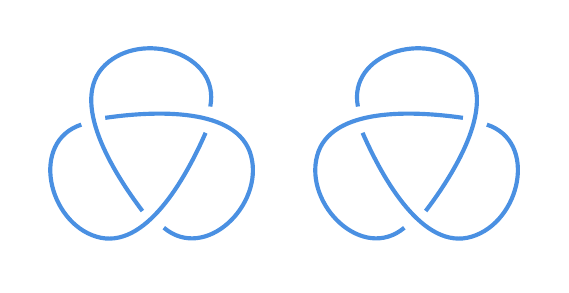
\begin{tikzpicture}[x=0.75pt,y=0.75pt,yscale=-1,xscale=1]
                %uncomment if require: \path (0,98); %set diagram left start at 0, and has height of 98
                
                %Curve Lines [id:da33652407494571124] 
                \draw [color={rgb, 255:red, 74; green, 144; blue, 226 }  ,draw opacity=1 ][line width=1.5]    (263.02,80.95) .. controls (248.71,62.08) and (227.36,27.62) .. (245.02,10.62) .. controls (262.69,-6.38) and (300.69,4.95) .. (295.69,30.62) ;
                %Curve Lines [id:da24624517583527616] 
                \draw [color={rgb, 255:red, 74; green, 144; blue, 226 }  ,draw opacity=1 ][line width=1.5]    (293.44,43.28) .. controls (283.94,64.98) and (264.29,100.44) .. (240.83,93.31) .. controls (217.37,86.19) and (208.72,47.49) .. (233.56,39.33) ;
                %Curve Lines [id:da7364718716830982] 
                \draw [color={rgb, 255:red, 74; green, 144; blue, 226 }  ,draw opacity=1 ][line width=1.5]    (245.08,36.06) .. controls (268.53,32.67) and (309.01,30.66) .. (315.34,54.35) .. controls (321.66,78.04) and (293.35,105.8) .. (273.31,89) ;
                
                %Curve Lines [id:da6177585740407667] 
                \draw [color={rgb, 255:red, 74; green, 144; blue, 226 }  ,draw opacity=1 ][line width=1.5]    (399.48,80.95) .. controls (413.79,62.08) and (435.15,27.62) .. (417.48,10.62) .. controls (399.82,-6.38) and (361.82,4.95) .. (366.82,30.62) ;
                %Curve Lines [id:da9792887763068585] 
                \draw [color={rgb, 255:red, 74; green, 144; blue, 226 }  ,draw opacity=1 ][line width=1.5]    (369.07,43.28) .. controls (378.56,64.98) and (398.22,100.44) .. (421.68,93.31) .. controls (445.14,86.19) and (453.79,47.49) .. (428.95,39.33) ;
                %Curve Lines [id:da846890298813785] 
                \draw [color={rgb, 255:red, 74; green, 144; blue, 226 }  ,draw opacity=1 ][line width=1.5]    (417.43,36.06) .. controls (393.98,32.67) and (353.49,30.66) .. (347.17,54.35) .. controls (340.84,78.04) and (369.16,105.8) .. (389.19,89) ;
        \end{tikzpicture}
        \caption{Left and Right Handed Trefoil Knots (on the left and right respectively)}
        \label{fig:leftAndRightHandedTrefoil}
\end{figure}

\paragraph{Remark} The word “trefoil” is from the plant trifolium, or clover, which has compound trifoliate leaves.

\paragraph{Answer}
We try to figure out the right trefoil first:
\begin{align*}
        \tikzset{every picture/.style={line width=0.75pt}} %set default line width to 0.75pt        
        \begin{tikzpicture}[x=0.75pt,y=0.75pt,yscale=-1,xscale=1, baseline=(XXXX.south) ]
                \path (0,68);\path (72.99199676513672,0);\draw    ($(current bounding box.center)+(0,0.3em)$) node [anchor=south] (XXXX) {};
                %Curve Lines [id:da17496258744516946] 
                \draw [color={rgb, 255:red, 74; green, 144; blue, 226 }  ,draw opacity=1 ][line width=1.5]    (38.33,55.68) .. controls (48.02,42.88) and (62.5,19.54) .. (50.52,8.02) .. controls (38.55,-3.5) and (12.8,4.18) .. (16.19,21.57) ;
                %Curve Lines [id:da6346543641723779] 
                \draw [color={rgb, 255:red, 74; green, 144; blue, 226 }  ,draw opacity=1 ][line width=1.5]    (17.72,30.15) .. controls (24.15,44.85) and (37.47,68.88) .. (53.37,64.05) .. controls (69.26,59.22) and (75.13,33) .. (58.29,27.47) ;
                %Curve Lines [id:da5357288157523301] 
                \draw [color={rgb, 255:red, 74; green, 144; blue, 226 }  ,draw opacity=1 ][line width=1.5]    (50.49,25.25) .. controls (34.6,22.96) and (7.16,21.6) .. (2.88,37.65) .. controls (-1.41,53.7) and (17.78,72.51) .. (31.36,61.13) ;
        \end{tikzpicture}
        = & A\tikzset{every picture/.style={line width=0.75pt}} %set default line width to 0.75pt        
        \begin{tikzpicture}[x=0.75pt,y=0.75pt,yscale=-1,xscale=1, baseline=(XXXX.south) ]
                \path (0,41);\path (49.990928649902344,0);\draw    ($(current bounding box.center)+(0,0.3em)$) node [anchor=south] (XXXX) {};
                %Shape: Arc [id:dp4141873258382096] 
                \draw  [draw opacity=0][line width=1.5]  (23.76,35.87) .. controls (20.84,37.23) and (17.76,38) .. (14.79,38) .. controls (5.57,38) and (0.87,30.55) .. (4.3,21.36) .. controls (7.73,12.16) and (17.99,4.71) .. (27.21,4.71) .. controls (36.43,4.71) and (41.13,12.16) .. (37.7,21.36) .. controls (36.18,25.41) and (33.34,29.13) .. (29.84,32.02) -- (21,21.36) -- cycle ; \draw  [color={rgb, 255:red, 74; green, 144; blue, 226 }  ,draw opacity=1 ][line width=1.5]  (23.76,35.87) .. controls (20.84,37.23) and (17.76,38) .. (14.79,38) .. controls (5.57,38) and (0.87,30.55) .. (4.3,21.36) .. controls (7.73,12.16) and (17.99,4.71) .. (27.21,4.71) .. controls (36.43,4.71) and (41.13,12.16) .. (37.7,21.36) .. controls (36.18,25.41) and (33.34,29.13) .. (29.84,32.02) ;  
                %Shape: Arc [id:dp2682249888444619] 
                \draw  [draw opacity=0][line width=1.5]  (41.46,20.34) .. controls (43.41,21.98) and (44.92,23.99) .. (45.67,26.17) .. controls (47.56,31.69) and (43.82,36.17) .. (37.31,36.17) .. controls (30.8,36.17) and (23.99,31.69) .. (22.1,26.17) .. controls (20.21,20.65) and (23.95,16.17) .. (30.46,16.17) .. controls (31.31,16.17) and (32.17,16.24) .. (33.01,16.39) -- (33.88,26.17) -- cycle ; \draw  [color={rgb, 255:red, 74; green, 144; blue, 226 }  ,draw opacity=1 ][line width=1.5]  (41.46,20.34) .. controls (43.41,21.98) and (44.92,23.99) .. (45.67,26.17) .. controls (47.56,31.69) and (43.82,36.17) .. (37.31,36.17) .. controls (30.8,36.17) and (23.99,31.69) .. (22.1,26.17) .. controls (20.21,20.65) and (23.95,16.17) .. (30.46,16.17) .. controls (31.31,16.17) and (32.17,16.24) .. (33.01,16.39) ;  
        \end{tikzpicture}
        +A^{-1}\tikzset{every picture/.style={line width=0.75pt}} %set default line width to 0.75pt        
        \begin{tikzpicture}[x=0.75pt,y=0.75pt,yscale=-1,xscale=1, baseline=(XXXX.south) ]
                \path (0,40);\path (43.99652099609375,0);\draw    ($(current bounding box.center)+(0,0.3em)$) node [anchor=south] (XXXX) {};
                %Curve Lines [id:da927026493955573] 
                \draw [color={rgb, 255:red, 74; green, 144; blue, 226 }  ,draw opacity=1 ][line width=1.5]    (24.4,30) .. controls (38.2,12.4) and (24.2,-1.8) .. (16.8,3.8) .. controls (9.4,9.4) and (12,18.4) .. (25.63,14.91) ;
                %Curve Lines [id:da09726340778421116] 
                \draw [color={rgb, 255:red, 74; green, 144; blue, 226 }  ,draw opacity=1 ][line width=1.5]    (34.4,19.2) .. controls (38.2,20.8) and (44,30.6) .. (35,35) .. controls (21,42.4) and (13.6,19) .. (9,18.8) .. controls (4,18.6) and (-6,38) .. (17.6,34.6) ;
        \end{tikzpicture}
        \\
        = & A\left( A\tikzset{every picture/.style={line width=0.75pt}} %set default line width to 0.75pt        
        \begin{tikzpicture}[x=0.75pt,y=0.75pt,yscale=-1,xscale=1, baseline=(XXXX.south) ]
                \path (0,48);\path (47.982688903808594,0);\draw    ($(current bounding box.center)+(0,0.3em)$) node [anchor=south] (XXXX) {};
                %Curve Lines [id:da3331281148347065] 
                \draw [color={rgb, 255:red, 74; green, 144; blue, 226 }  ,draw opacity=1 ][line width=1.5]    (18.44,39.99) .. controls (15.49,41.39) and (5.24,41.43) .. (3.54,35.24) .. controls (1.84,29.05) and (5.16,26.6) .. (10.88,18.99) .. controls (16.61,11.37) and (16.06,4.58) .. (23.73,4.37) .. controls (31.39,4.15) and (31.28,11.92) .. (35.92,18.4) .. controls (40.56,24.88) and (49.52,34.59) .. (40.35,39.56) .. controls (31.17,44.52) and (24.27,39.56) .. (19.19,34.38) .. controls (14.12,29.19) and (13.04,17.97) .. (21.24,17.75) .. controls (29.45,17.54) and (31.39,19.8) .. (31.93,24.34) .. controls (32.47,28.87) and (29.66,31.79) .. (26.75,35.13) ;
        \end{tikzpicture}
        +A^{-1}\tikzset{every picture/.style={line width=0.75pt}} %set default line width to 0.75pt        
        \begin{tikzpicture}[x=0.75pt,y=0.75pt,yscale=-1,xscale=1, baseline=(XXXX.south) ]
                \path (0,40);\path (41.9948844909668,0);\draw    ($(current bounding box.center)+(0,0.3em)$) node [anchor=south] (XXXX) {};
                %Curve Lines [id:da5741582875020317] 
                \draw [color={rgb, 255:red, 74; green, 144; blue, 226 }  ,draw opacity=1 ][line width=1.5]    (23.37,29.81) .. controls (28.38,26.05) and (29.18,19.24) .. (33.44,19.71) .. controls (37.7,20.19) and (42.31,28.46) .. (36.99,33.21) .. controls (31.68,37.95) and (20.18,34.63) .. (16.63,27.29) .. controls (13.08,19.95) and (16.39,19) .. (18.29,17.34) .. controls (20.18,15.69) and (29.89,14.98) .. (29.42,11.43) .. controls (28.94,7.87) and (24.21,1.48) .. (19.23,2.66) .. controls (14.26,3.85) and (14.03,9.77) .. (11.66,14.5) .. controls (9.29,19.24) and (2.42,20.42) .. (2.66,27.53) .. controls (2.9,34.63) and (10.71,37.23) .. (16.76,34.16) ;
        \end{tikzpicture}
        \right) +A^{-1}\left( A\tikzset{every picture/.style={line width=0.75pt}} %set default line width to 0.75pt        
        \begin{tikzpicture}[x=0.75pt,y=0.75pt,yscale=-1,xscale=1, baseline=(XXXX.south) ]
                \path (0,40);\path (43.99652099609375,0);\draw    ($(current bounding box.center)+(0,0.3em)$) node [anchor=south] (XXXX) {};
                %Curve Lines [id:da5645836951254308] 
                \draw [color={rgb, 255:red, 74; green, 144; blue, 226 }  ,draw opacity=1 ][line width=1.5]    (16.43,35.98) .. controls (11.22,37.55) and (5.31,35.1) .. (3.66,30.99) .. controls (2.02,26.88) and (4.81,19.83) .. (9.5,19.66) .. controls (14.18,19.48) and (17.66,40.66) .. (34,35.99) .. controls (50.33,31.32) and (35.16,1.16) .. (22.66,2.99) .. controls (10.16,4.82) and (12.16,14.99) .. (15.5,15.49) .. controls (18.83,15.99) and (25.5,14.49) .. (27.66,18.32) .. controls (29.83,22.16) and (28.33,25.99) .. (23.5,30.82) ;
        \end{tikzpicture}
        +A^{-1}\tikzset{every picture/.style={line width=0.75pt}} %set default line width to 0.75pt        
        \begin{tikzpicture}[x=0.75pt,y=0.75pt,yscale=-1,xscale=1, baseline=(XXXX.south) ]
                \path (0,40);\path (43.99652099609375,0);\draw    ($(current bounding box.center)+(0,0.3em)$) node [anchor=south] (XXXX) {};
                %Curve Lines [id:da4563387979551714] 
                \draw [color={rgb, 255:red, 74; green, 144; blue, 226 }  ,draw opacity=1 ][line width=1.5]    (23,30.32) .. controls (28.66,23.32) and (30.66,14.66) .. (36,18.99) .. controls (41.33,23.32) and (40,33.82) .. (33.5,34.99) .. controls (26.99,36.16) and (22.83,33.32) .. (18.5,30.32) .. controls (14.16,27.32) and (11.67,15.29) .. (5.66,18.99) .. controls (-0.35,22.7) and (2.83,39.99) .. (16.5,34.32) ;
                %Curve Lines [id:da372717649034797] 
                \draw [color={rgb, 255:red, 74; green, 144; blue, 226 }  ,draw opacity=1 ][line width=1.5]    (20.16,14.49) .. controls (34.5,14.16) and (27.66,1.99) .. (20.16,1.99) .. controls (12.66,1.99) and (6.33,14.99) .. (20.16,14.49) -- cycle ;
        \end{tikzpicture}
        \right)\\
        = & A^{2}\left( A\tikzset{every picture/.style={line width=0.75pt}} %set default line width to 0.75pt        
        \begin{tikzpicture}[x=0.75pt,y=0.75pt,yscale=-1,xscale=1, baseline=(XXXX.south) ]
                \path (0,40);\path (43.99652099609375,0);\draw    ($(current bounding box.center)+(0,0.3em)$) node [anchor=south] (XXXX) {};
                %Shape: Circle [id:dp6253531078371917] 
                \draw  [color={rgb, 255:red, 74; green, 144; blue, 226 }  ,draw opacity=1 ][line width=1.5]  (5.3,20.64) .. controls (5.3,11.06) and (13.06,3.29) .. (22.65,3.29) .. controls (32.23,3.29) and (40,11.06) .. (40,20.64) .. controls (40,30.22) and (32.23,37.99) .. (22.65,37.99) .. controls (13.06,37.99) and (5.3,30.22) .. (5.3,20.64) -- cycle ;
                %Shape: Circle [id:dp34206862302889895] 
                \draw  [color={rgb, 255:red, 74; green, 144; blue, 226 }  ,draw opacity=1 ][line width=1.5]  (14.97,20.64) .. controls (14.97,16.4) and (18.41,12.96) .. (22.65,12.96) .. controls (26.88,12.96) and (30.32,16.4) .. (30.32,20.64) .. controls (30.32,24.88) and (26.88,28.32) .. (22.65,28.32) .. controls (18.41,28.32) and (14.97,24.88) .. (14.97,20.64) -- cycle ;
        \end{tikzpicture}
        +A^{-1}\tikzset{every picture/.style={line width=0.75pt}} %set default line width to 0.75pt        
        \begin{tikzpicture}[x=0.75pt,y=0.75pt,yscale=-1,xscale=1, baseline=(XXXX.south) ]
                \path (0,40);\path (43.99652099609375,0);\draw    ($(current bounding box.center)+(0,0.3em)$) node [anchor=south] (XXXX) {};
                %Shape: Circle [id:dp3384239181781197] 
                \draw  [color={rgb, 255:red, 74; green, 144; blue, 226 }  ,draw opacity=1 ][line width=1.5]  (5.3,21.64) .. controls (5.3,12.06) and (13.06,4.29) .. (22.65,4.29) .. controls (32.23,4.29) and (40,12.06) .. (40,21.64) .. controls (40,31.22) and (32.23,38.99) .. (22.65,38.99) .. controls (13.06,38.99) and (5.3,31.22) .. (5.3,21.64) -- cycle ;
        \end{tikzpicture}
        \right) +\left( A\tikzset{every picture/.style={line width=0.75pt}} %set default line width to 0.75pt        
        \begin{tikzpicture}[x=0.75pt,y=0.75pt,yscale=-1,xscale=1, baseline=(XXXX.south) ]
                \path (0,40);\path (43.99652099609375,0);\draw    ($(current bounding box.center)+(0,0.3em)$) node [anchor=south] (XXXX) {};
                %Shape: Circle [id:dp5240073107156691] 
                \draw  [color={rgb, 255:red, 74; green, 144; blue, 226 }  ,draw opacity=1 ][line width=1.5]  (5.3,21.64) .. controls (5.3,12.06) and (13.06,4.29) .. (22.65,4.29) .. controls (32.23,4.29) and (40,12.06) .. (40,21.64) .. controls (40,31.22) and (32.23,38.99) .. (22.65,38.99) .. controls (13.06,38.99) and (5.3,31.22) .. (5.3,21.64) -- cycle ;
        \end{tikzpicture}
        +A^{-1}\tikzset{every picture/.style={line width=0.75pt}} %set default line width to 0.75pt        
        \begin{tikzpicture}[x=0.75pt,y=0.75pt,yscale=-1,xscale=1, baseline=(XXXX.south) ]
                \path (0,31);\path (59.99232482910156,0);\draw    ($(current bounding box.center)+(0,0.3em)$) node [anchor=south] (XXXX) {};
                %Shape: Circle [id:dp17633990879069805] 
                \draw  [color={rgb, 255:red, 74; green, 144; blue, 226 }  ,draw opacity=1 ][line width=1.5]  (3.3,16.14) .. controls (3.3,10.15) and (8.15,5.29) .. (14.15,5.29) .. controls (20.14,5.29) and (25,10.15) .. (25,16.14) .. controls (25,22.13) and (20.14,26.99) .. (14.15,26.99) .. controls (8.15,26.99) and (3.3,22.13) .. (3.3,16.14) -- cycle ;
                %Shape: Circle [id:dp09348561797596755] 
                \draw  [color={rgb, 255:red, 74; green, 144; blue, 226 }  ,draw opacity=1 ][line width=1.5]  (32.3,16.14) .. controls (32.3,10.15) and (37.15,5.29) .. (43.15,5.29) .. controls (49.14,5.29) and (54,10.15) .. (54,16.14) .. controls (54,22.13) and (49.14,26.99) .. (43.15,26.99) .. controls (37.15,26.99) and (32.3,22.13) .. (32.3,16.14) -- cycle ;
        \end{tikzpicture}
        \right)\\
        & +\left( A\tikzset{every picture/.style={line width=0.75pt}} %set default line width to 0.75pt        
        \begin{tikzpicture}[x=0.75pt,y=0.75pt,yscale=-1,xscale=1, baseline=(XXXX.south) ]
                \path (0,40);\path (43.99652099609375,0);\draw    ($(current bounding box.center)+(0,0.3em)$) node [anchor=south] (XXXX) {};
                %Shape: Circle [id:dp7807071920749482] 
                \draw  [color={rgb, 255:red, 74; green, 144; blue, 226 }  ,draw opacity=1 ][line width=1.5]  (5.3,20.64) .. controls (5.3,11.06) and (13.06,3.29) .. (22.65,3.29) .. controls (32.23,3.29) and (40,11.06) .. (40,20.64) .. controls (40,30.22) and (32.23,37.99) .. (22.65,37.99) .. controls (13.06,37.99) and (5.3,30.22) .. (5.3,20.64) -- cycle ;
        \end{tikzpicture}
        +A^{-1}\tikzset{every picture/.style={line width=0.75pt}} %set default line width to 0.75pt        
        \begin{tikzpicture}[x=0.75pt,y=0.75pt,yscale=-1,xscale=1, baseline=(XXXX.south) ]
                \path (0,31);\path (59.99232482910156,0);\draw    ($(current bounding box.center)+(0,0.3em)$) node [anchor=south] (XXXX) {};
                %Shape: Circle [id:dp14222723555272965] 
                \draw  [color={rgb, 255:red, 74; green, 144; blue, 226 }  ,draw opacity=1 ][line width=1.5]  (3.3,16.14) .. controls (3.3,10.15) and (8.15,5.29) .. (14.15,5.29) .. controls (20.14,5.29) and (25,10.15) .. (25,16.14) .. controls (25,22.13) and (20.14,26.99) .. (14.15,26.99) .. controls (8.15,26.99) and (3.3,22.13) .. (3.3,16.14) -- cycle ;
                %Shape: Circle [id:dp13034301114351332] 
                \draw  [color={rgb, 255:red, 74; green, 144; blue, 226 }  ,draw opacity=1 ][line width=1.5]  (32.3,16.14) .. controls (32.3,10.15) and (37.15,5.29) .. (43.15,5.29) .. controls (49.14,5.29) and (54,10.15) .. (54,16.14) .. controls (54,22.13) and (49.14,26.99) .. (43.15,26.99) .. controls (37.15,26.99) and (32.3,22.13) .. (32.3,16.14) -- cycle ;
        \end{tikzpicture}
        \right) +A^{-2}\left( A\tikzset{every picture/.style={line width=0.75pt}} %set default line width to 0.75pt        
        \begin{tikzpicture}[x=0.75pt,y=0.75pt,yscale=-1,xscale=1, baseline=(XXXX.south) ]
                \path (0,44);\path (26.994884490966797,0);\draw    ($(current bounding box.center)+(0,0.3em)$) node [anchor=south] (XXXX) {};
                %Shape: Circle [id:dp8462936980147189] 
                \draw  [color={rgb, 255:red, 74; green, 144; blue, 226 }  ,draw opacity=1 ][line width=1.5]  (12.93,2.79) .. controls (17.43,2.79) and (21.07,6.43) .. (21.07,10.93) .. controls (21.07,15.42) and (17.43,19.06) .. (12.93,19.06) .. controls (8.44,19.06) and (4.8,15.42) .. (4.8,10.93) .. controls (4.8,6.43) and (8.44,2.79) .. (12.93,2.79) -- cycle ;
                %Shape: Circle [id:dp8544095207014937] 
                \draw  [color={rgb, 255:red, 74; green, 144; blue, 226 }  ,draw opacity=1 ][line width=1.5]  (12.93,24.54) .. controls (17.43,24.54) and (21.07,28.18) .. (21.07,32.67) .. controls (21.07,37.17) and (17.43,40.81) .. (12.93,40.81) .. controls (8.44,40.81) and (4.8,37.17) .. (4.8,32.67) .. controls (4.8,28.18) and (8.44,24.54) .. (12.93,24.54) -- cycle ;
        \end{tikzpicture}
        +A^{-1}\tikzset{every picture/.style={line width=0.75pt}} %set default line width to 0.75pt        
        \begin{tikzpicture}[x=0.75pt,y=0.75pt,yscale=-1,xscale=1, baseline=(XXXX.south) ]
                \path (0,42);\path (47.98960876464844,0);\draw    ($(current bounding box.center)+(0,0.3em)$) node [anchor=south] (XXXX) {};
                %Shape: Circle [id:dp2808548197181753] 
                \draw  [color={rgb, 255:red, 74; green, 144; blue, 226 }  ,draw opacity=1 ][line width=1.5]  (22.93,1.96) .. controls (27.43,1.96) and (31.07,5.61) .. (31.07,10.1) .. controls (31.07,14.6) and (27.43,18.24) .. (22.93,18.24) .. controls (18.44,18.24) and (14.8,14.6) .. (14.8,10.1) .. controls (14.8,5.61) and (18.44,1.96) .. (22.93,1.96) -- cycle ;
                %Shape: Circle [id:dp4701752603617959] 
                \draw  [color={rgb, 255:red, 74; green, 144; blue, 226 }  ,draw opacity=1 ][line width=1.5]  (10.93,23.71) .. controls (15.43,23.71) and (19.07,27.36) .. (19.07,31.85) .. controls (19.07,36.34) and (15.43,39.99) .. (10.93,39.99) .. controls (6.44,39.99) and (2.8,36.34) .. (2.8,31.85) .. controls (2.8,27.36) and (6.44,23.71) .. (10.93,23.71) -- cycle ;
                %Shape: Circle [id:dp8102265525674299] 
                \draw  [color={rgb, 255:red, 74; green, 144; blue, 226 }  ,draw opacity=1 ][line width=1.5]  (35.86,23.71) .. controls (40.35,23.71) and (43.99,27.35) .. (43.99,31.85) .. controls (43.99,36.34) and (40.35,39.98) .. (35.86,39.98) .. controls (31.36,39.98) and (27.72,36.34) .. (27.72,31.85) .. controls (27.72,27.35) and (31.36,23.71) .. (35.86,23.71) -- cycle ;
        \end{tikzpicture}
        \right)\\
        = & A^{2} (Ad^{2} +A^{-1} d)+(Ad+A^{-1} d^{2} )+(Ad +A^{-1} d^{2} )+A^{-2} (Ad^{2} +A^{-1} d^{3} )\\
        = & -A^{-9} +A^{-1}+A^{3} +A^{7} .
\end{align*}
Similar calculation gives
\begin{equation*}
        \tikzset{every picture/.style={line width=0.75pt}} %set default line width to 0.75pt        
        \begin{tikzpicture}[x=0.75pt,y=0.75pt,yscale=-1,xscale=1, baseline=(XXXX.south) ]
                \path (0,68);\path (72.99199676513672,0);\draw    ($(current bounding box.center)+(0,0.3em)$) node [anchor=south] (XXXX) {};
                %Curve Lines [id:da43968276064415623] 
                \draw [color={rgb, 255:red, 74; green, 144; blue, 226 }  ,draw opacity=1 ][line width=1.5]    (32.37,55.68) .. controls (22.67,42.88) and (8.2,19.54) .. (20.17,8.02) .. controls (32.14,-3.5) and (57.89,4.18) .. (54.5,21.57) ;
                %Curve Lines [id:da5050406190521861] 
                \draw [color={rgb, 255:red, 74; green, 144; blue, 226 }  ,draw opacity=1 ][line width=1.5]    (52.98,30.15) .. controls (46.54,44.85) and (33.23,68.88) .. (17.33,64.05) .. controls (1.43,59.22) and (-4.43,33) .. (12.4,27.47) ;
                %Curve Lines [id:da7698083169944674] 
                \draw [color={rgb, 255:red, 74; green, 144; blue, 226 }  ,draw opacity=1 ][line width=1.5]    (20.21,25.25) .. controls (36.1,22.96) and (63.53,21.6) .. (67.82,37.65) .. controls (72.1,53.7) and (52.92,72.51) .. (39.34,61.13) ;
        \end{tikzpicture}
        =-A^{9} +A^{1} +A^{-3} +A^{-7} .
\end{equation*}
We can see the mirror symmetry gives $A\rightarrow A^{-1}$. In other notations, we can set $d^{i}\rightarrow d^{i-1}$, then the trivial knot(i.e. a circle) give $1$. Then we have
\begin{equation*}
        \tikzset{every picture/.style={line width=0.75pt}} %set default line width to 0.75pt        
        \begin{tikzpicture}[x=0.75pt,y=0.75pt,yscale=-1,xscale=1, baseline=(XXXX.south) ]
                \path (0,68);\path (72.99199676513672,0);\draw    ($(current bounding box.center)+(0,0.3em)$) node [anchor=south] (XXXX) {};
                %Curve Lines [id:da9633941749826875] 
                \draw [color={rgb, 255:red, 74; green, 144; blue, 226 }  ,draw opacity=1 ][line width=1.5]    (38.33,55.68) .. controls (48.02,42.88) and (62.5,19.54) .. (50.52,8.02) .. controls (38.55,-3.5) and (12.8,4.18) .. (16.19,21.57) ;
                %Curve Lines [id:da6880787601193201] 
                \draw [color={rgb, 255:red, 74; green, 144; blue, 226 }  ,draw opacity=1 ][line width=1.5]    (17.72,30.15) .. controls (24.15,44.85) and (37.47,68.88) .. (53.37,64.05) .. controls (69.26,59.22) and (75.13,33) .. (58.29,27.47) ;
                %Curve Lines [id:da8809202495162078] 
                \draw [color={rgb, 255:red, 74; green, 144; blue, 226 }  ,draw opacity=1 ][line width=1.5]    (50.49,25.25) .. controls (34.6,22.96) and (7.16,21.6) .. (2.88,37.65) .. controls (-1.41,53.7) and (17.78,72.51) .. (31.36,61.13) ;
        \end{tikzpicture}
        =A^{-7} -A^{5} -A^{3} .
\end{equation*}

\section{Abelian Kauffman Anyons}
Anyons described by the Kauffman bracket invariant with certain special values of the constant $A$ are abelian anyons - meaning that an exchange introduces only a simple phase as shown in Fig. \ref{fig:AbelianAnyonExchange}.

\begin{figure}[h!]
        \centering
        \tikzset{every picture/.style={line width=0.75pt}} %set default line width to 0.75pt        
        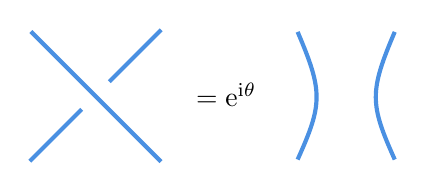
\begin{tikzpicture}[x=0.75pt,y=0.75pt,yscale=-1,xscale=1]
                %uncomment if require: \path (0,68); %set diagram left start at 0, and has height of 68
                
                %Straight Lines [id:da12351686453929012] 
                \draw [color={rgb, 255:red, 74; green, 144; blue, 226 }  ,draw opacity=1 ][line width=1.5]    (240.67,3.65) -- (303.37,66.35) ;
                %Straight Lines [id:da5675480043864236] 
                \draw [color={rgb, 255:red, 74; green, 144; blue, 226 }  ,draw opacity=1 ][line width=1.5]    (278.45,27.79) -- (303.45,2.79) ;
                %Straight Lines [id:da37770163193150785] 
                \draw [color={rgb, 255:red, 74; green, 144; blue, 226 }  ,draw opacity=1 ][line width=1.5]    (240.11,66.12) -- (265.11,41.12) ;
                
                %Curve Lines [id:da4265407093388114] 
                \draw [color={rgb, 255:red, 74; green, 144; blue, 226 }  ,draw opacity=1 ][line width=1.5]    (369.17,3.82) .. controls (381.5,32.65) and (381.17,38.65) .. (369.17,65.32) ;
                %Curve Lines [id:da5245986537990159] 
                \draw [color={rgb, 255:red, 74; green, 144; blue, 226 }  ,draw opacity=1 ][line width=1.5]    (415.96,3.82) .. controls (403.63,32.65) and (403.96,38.65) .. (415.96,65.32) ;
                
                
                % Text Node
                \draw (318.81,27.07) node [anchor=north west][inner sep=0.75pt]    {$=\mathrm{e}^{\mathrm{i} \theta }$};
        \end{tikzpicture}
        \caption{For abelian anyons, exchange gives a phase $\mathrm{e}^{\mathrm{i} \theta }$.}
        \label{fig:AbelianAnyonExchange}
\end{figure}

\begin{enumerate}
        \item For $A=\pm \mathrm{e}^{\mathrm{i} \pi /3}$ (and the complex conjugates of these values), show that the anyons are bosons or fermions respectively (i.e., $\mathrm{e}^{\mathrm{i} \theta } =\pm 1$ ).
        \item For $A=\pm \mathrm{e}^{\mathrm{i} \pi /6}$ (and the complex conjugates of these values) show the anyons are semions (i.e., $\mathrm{e}^{\mathrm{i} \theta } =\pm \mathrm{i}$ ). In fact these are precisely the anyons that arise for the $\nu =1/2$ fractional quantum Hall effect of bosons (We will discuss this later in this book (See chapter 37). This particular phase of quantum Hall matter has been produced experimentally(Clark et al. [2020]), but only in very small puddles so far and it has not been possible to measure braiding statistics as of yet.
\end{enumerate}
HINT: For (a) and (b) show first the identity shown in Fig. \ref{fig:ExchangeBosonsOrFermions}.

If you can't figure it out, try evaluating the Kauffman bracket invariant for a few knots with these values of $A$ and see how the result arises.

\begin{figure}[h!]
        \centering
        \tikzset{every picture/.style={line width=0.75pt}} %set default line width to 0.75pt        
        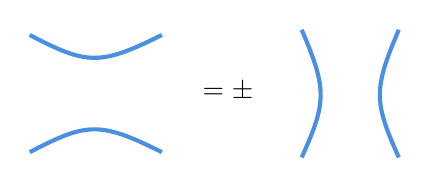
\begin{tikzpicture}[x=0.75pt,y=0.75pt,yscale=-1,xscale=1]
                %uncomment if require: \path (0,65); %set diagram left start at 0, and has height of 65
                %Curve Lines [id:da8961261533012252] 
                \draw [color={rgb, 255:red, 74; green, 144; blue, 226 }  ,draw opacity=1 ][line width=1.5]    (305.81,4.41) .. controls (275.96,19.3) and (269.75,18.9) .. (242.15,4.41) ;
                %Curve Lines [id:da47083895189428304] 
                \draw [color={rgb, 255:red, 74; green, 144; blue, 226 }  ,draw opacity=1 ][line width=1.5]    (305.81,60.89) .. controls (275.96,46.01) and (269.75,46.41) .. (242.15,60.89) ;
                
                %Curve Lines [id:da9898702962562469] 
                \draw [color={rgb, 255:red, 74; green, 144; blue, 226 }  ,draw opacity=1 ][line width=1.5]    (373.17,1.9) .. controls (385.5,30.74) and (385.17,36.74) .. (373.17,63.4) ;
                %Curve Lines [id:da26291761978783246] 
                \draw [color={rgb, 255:red, 74; green, 144; blue, 226 }  ,draw opacity=1 ][line width=1.5]    (419.96,1.9) .. controls (407.63,30.74) and (407.96,36.74) .. (419.96,63.4) ;
                % Text Node
                \draw (324,25.65) node [anchor=north west][inner sep=0.75pt]    {$=\pm $};
        \end{tikzpicture}
        \caption{For bosons or fermions the sign in this figure is $+$, for semions the sign is $-$.}
        \label{fig:ExchangeBosonsOrFermions}
\end{figure}

\paragraph{Answer}
Using the definition of Kauffman bracket:
\begin{equation*}
        \begin{aligned}
                \tikzset{every picture/.style={line width=0.75pt}} %set default line width to 0.75pt        
                \begin{tikzpicture}[x=0.75pt,y=0.75pt,yscale=-1,xscale=1, baseline=(XXXX.south) ]
                        \path (0,68);\path (68.99652099609375,0);\draw    ($(current bounding box.center)+(0,0.3em)$) node [anchor=south] (XXXX) {};
                        %Straight Lines [id:da7539388624541459] 
                        \draw [color={rgb, 255:red, 74; green, 144; blue, 226 }  ,draw opacity=1 ][line width=1.5]    (65.7,3.81) -- (3,66.51) ;
                        %Straight Lines [id:da3938438906428654] 
                        \draw [color={rgb, 255:red, 74; green, 144; blue, 226 }  ,draw opacity=1 ][line width=1.5]    (41.56,41.59) -- (66.56,66.59) ;
                        %Straight Lines [id:da18516570828706413] 
                        \draw [color={rgb, 255:red, 74; green, 144; blue, 226 }  ,draw opacity=1 ][line width=1.5]    (3.23,3.25) -- (28.23,28.25) ;
                \end{tikzpicture}
                & =A\tikzset{every picture/.style={line width=0.75pt}} %set default line width to 0.75pt        
                \begin{tikzpicture}[x=0.75pt,y=0.75pt,yscale=-1,xscale=1, baseline=(XXXX.south) ]
                        \path (0,68);\path (53.991668701171875,0);\draw    ($(current bounding box.center)+(0,0.3em)$) node [anchor=south] (XXXX) {};
                        %Curve Lines [id:da37581413358541704] 
                        \draw [color={rgb, 255:red, 74; green, 144; blue, 226 }  ,draw opacity=1 ][line width=1.5]    (4.17,2.29) .. controls (16.5,31.12) and (16.17,37.12) .. (4.17,63.79) ;
                        %Curve Lines [id:da9006964162238551] 
                        \draw [color={rgb, 255:red, 74; green, 144; blue, 226 }  ,draw opacity=1 ][line width=1.5]    (50.96,2.29) .. controls (38.63,31.12) and (38.96,37.12) .. (50.96,63.79) ;
                \end{tikzpicture}
                +A^{-1}\tikzset{every picture/.style={line width=0.75pt}} %set default line width to 0.75pt        
                \begin{tikzpicture}[x=0.75pt,y=0.75pt,yscale=-1,xscale=1, baseline=(XXXX.south) ]
                        \path (0,67);\path (71.98169708251953,0);\draw    ($(current bounding box.center)+(0,0.3em)$) node [anchor=south] (XXXX) {};
                        %Curve Lines [id:da0002888383512205106] 
                        \draw [color={rgb, 255:red, 74; green, 144; blue, 226 }  ,draw opacity=1 ][line width=1.5]    (68.81,4.31) .. controls (38.96,19.2) and (32.75,18.79) .. (5.15,4.31) ;
                        %Curve Lines [id:da2642472194401073] 
                        \draw [color={rgb, 255:red, 74; green, 144; blue, 226 }  ,draw opacity=1 ][line width=1.5]    (68.81,60.79) .. controls (38.96,45.9) and (32.75,46.3) .. (5.15,60.79) ;
                \end{tikzpicture}
                \\
                & \stackrel{!}{=}\mathrm{e}^{\mathrm{i} \theta }\tikzset{every picture/.style={line width=0.75pt}} %set default line width to 0.75pt        
                \begin{tikzpicture}[x=0.75pt,y=0.75pt,yscale=-1,xscale=1, baseline=(XXXX.south) ]
                        \path (0,68);\path (53.991668701171875,0);\draw    ($(current bounding box.center)+(0,0.3em)$) node [anchor=south] (XXXX) {};
                        %Curve Lines [id:da5214125017288944] 
                        \draw [color={rgb, 255:red, 74; green, 144; blue, 226 }  ,draw opacity=1 ][line width=1.5]    (4.17,2.29) .. controls (16.5,31.12) and (16.17,37.12) .. (4.17,63.79) ;
                        %Curve Lines [id:da2916432495183652] 
                        \draw [color={rgb, 255:red, 74; green, 144; blue, 226 }  ,draw opacity=1 ][line width=1.5]    (50.96,2.29) .. controls (38.63,31.12) and (38.96,37.12) .. (50.96,63.79) ;
                \end{tikzpicture}
                ,
        \end{aligned}
\end{equation*}
which means we have:
\begin{equation*}
        \tikzset{every picture/.style={line width=0.75pt}} %set default line width to 0.75pt        
        \begin{tikzpicture}[x=0.75pt,y=0.75pt,yscale=-1,xscale=1, baseline=(XXXX.south) ]
                \path (0,68);\path (53.991668701171875,0);\draw    ($(current bounding box.center)+(0,0.3em)$) node [anchor=south] (XXXX) {};
                %Curve Lines [id:da3520499283776384] 
                \draw [color={rgb, 255:red, 74; green, 144; blue, 226 }  ,draw opacity=1 ][line width=1.5]    (4.17,2.29) .. controls (16.5,31.12) and (16.17,37.12) .. (4.17,63.79) ;
                %Curve Lines [id:da7874206506093477] 
                \draw [color={rgb, 255:red, 74; green, 144; blue, 226 }  ,draw opacity=1 ][line width=1.5]    (50.96,2.29) .. controls (38.63,31.12) and (38.96,37.12) .. (50.96,63.79) ;
        \end{tikzpicture}
        =\frac{A^{-1}}{\mathrm{e}^{\mathrm{i} \theta } -A}\tikzset{every picture/.style={line width=0.75pt}} %set default line width to 0.75pt        
        \begin{tikzpicture}[x=0.75pt,y=0.75pt,yscale=-1,xscale=1, baseline=(XXXX.south) ]
                \path (0,67);\path (71.98169708251953,0);\draw    ($(current bounding box.center)+(0,0.3em)$) node [anchor=south] (XXXX) {};
                %Curve Lines [id:da9101758088105385] 
                \draw [color={rgb, 255:red, 74; green, 144; blue, 226 }  ,draw opacity=1 ][line width=1.5]    (68.81,4.31) .. controls (38.96,19.2) and (32.75,18.79) .. (5.15,4.31) ;
                %Curve Lines [id:da9071304110135325] 
                \draw [color={rgb, 255:red, 74; green, 144; blue, 226 }  ,draw opacity=1 ][line width=1.5]    (68.81,60.79) .. controls (38.96,45.9) and (32.75,46.3) .. (5.15,60.79) ;
        \end{tikzpicture}
        .
\end{equation*}
At the same time, we also have
\begin{equation*}
        \begin{aligned}
                \tikzset{every picture/.style={line width=0.75pt}} %set default line width to 0.75pt 
                \begin{tikzpicture}[x=0.75pt,y=0.75pt,yscale=-1,xscale=1, baseline=(XXXX.south) ]
                        \path (0,68);\path (68.99652099609375,0);\draw    ($(current bounding box.center)+(0,0.3em)$) node [anchor=south] (XXXX) {};
                        %Straight Lines [id:da5470670447844541] 
                        \draw [color={rgb, 255:red, 74; green, 144; blue, 226 }  ,draw opacity=1 ][line width=1.5]    (3.67,4) -- (66.37,66.7) ;
                        %Straight Lines [id:da013140972627327496] 
                        \draw [color={rgb, 255:red, 74; green, 144; blue, 226 }  ,draw opacity=1 ][line width=1.5]    (41.45,28.14) -- (66.45,3.14) ;
                        %Straight Lines [id:da8599231631706779] 
                        \draw [color={rgb, 255:red, 74; green, 144; blue, 226 }  ,draw opacity=1 ][line width=1.5]    (3.11,66.47) -- (28.11,41.47) ;
                \end{tikzpicture}       
                & =A\tikzset{every picture/.style={line width=0.75pt}} %set default line width to 0.75pt        
                \begin{tikzpicture}[x=0.75pt,y=0.75pt,yscale=-1,xscale=1, baseline=(XXXX.south) ]
                        \path (0,67);\path (71.98169708251953,0);\draw    ($(current bounding box.center)+(0,0.3em)$) node [anchor=south] (XXXX) {};
                        %Curve Lines [id:da8933911166454194] 
                        \draw [color={rgb, 255:red, 74; green, 144; blue, 226 }  ,draw opacity=1 ][line width=1.5]    (68.81,4.31) .. controls (38.96,19.2) and (32.75,18.79) .. (5.15,4.31) ;
                        %Curve Lines [id:da4551593879680247] 
                        \draw [color={rgb, 255:red, 74; green, 144; blue, 226 }  ,draw opacity=1 ][line width=1.5]    (68.81,60.79) .. controls (38.96,45.9) and (32.75,46.3) .. (5.15,60.79) ;
                \end{tikzpicture}
                +A^{-1}\tikzset{every picture/.style={line width=0.75pt}} %set default line width to 0.75pt        
                \begin{tikzpicture}[x=0.75pt,y=0.75pt,yscale=-1,xscale=1, baseline=(XXXX.south) ]
                        \path (0,68);\path (53.991668701171875,0);\draw    ($(current bounding box.center)+(0,0.3em)$) node [anchor=south] (XXXX) {};
                        %Curve Lines [id:da7648739395234672] 
                        \draw [color={rgb, 255:red, 74; green, 144; blue, 226 }  ,draw opacity=1 ][line width=1.5]    (4.17,2.29) .. controls (16.5,31.12) and (16.17,37.12) .. (4.17,63.79) ;
                        %Curve Lines [id:da5044659836989394] 
                        \draw [color={rgb, 255:red, 74; green, 144; blue, 226 }  ,draw opacity=1 ][line width=1.5]    (50.96,2.29) .. controls (38.63,31.12) and (38.96,37.12) .. (50.96,63.79) ;
                \end{tikzpicture}
                \\
                & \stackrel{!}{=}\mathrm{e}^{-\mathrm{i} \theta }\tikzset{every picture/.style={line width=0.75pt}} %set default line width to 0.75pt        
                \begin{tikzpicture}[x=0.75pt,y=0.75pt,yscale=-1,xscale=1, baseline=(XXXX.south) ]
                        \path (0,68);\path (53.991668701171875,0);\draw    ($(current bounding box.center)+(0,0.3em)$) node [anchor=south] (XXXX) {};
                        %Curve Lines [id:da48143120116797333] 
                        \draw [color={rgb, 255:red, 74; green, 144; blue, 226 }  ,draw opacity=1 ][line width=1.5]    (4.17,2.29) .. controls (16.5,31.12) and (16.17,37.12) .. (4.17,63.79) ;
                        %Curve Lines [id:da5734280588341469] 
                        \draw [color={rgb, 255:red, 74; green, 144; blue, 226 }  ,draw opacity=1 ][line width=1.5]    (50.96,2.29) .. controls (38.63,31.12) and (38.96,37.12) .. (50.96,63.79) ;
                \end{tikzpicture}
                ,
        \end{aligned}
\end{equation*}
Because exchange two particles in one certain direction gives a phase factor $\mathrm{e}^{\mathrm{i} \theta }$. Then
\begin{equation*}
        \tikzset{every picture/.style={line width=0.75pt}} %set default line width to 0.75pt        
        \begin{tikzpicture}[x=0.75pt,y=0.75pt,yscale=-1,xscale=1, baseline=(XXXX.south) ]
                \path (0,68);\path (53.991668701171875,0);\draw    ($(current bounding box.center)+(0,0.3em)$) node [anchor=south] (XXXX) {};
                %Curve Lines [id:da3082007174180428] 
                \draw [color={rgb, 255:red, 74; green, 144; blue, 226 }  ,draw opacity=1 ][line width=1.5]    (4.17,2.29) .. controls (16.5,31.12) and (16.17,37.12) .. (4.17,63.79) ;
                %Curve Lines [id:da2760148242111715] 
                \draw [color={rgb, 255:red, 74; green, 144; blue, 226 }  ,draw opacity=1 ][line width=1.5]    (50.96,2.29) .. controls (38.63,31.12) and (38.96,37.12) .. (50.96,63.79) ;
        \end{tikzpicture}
        =\frac{A}{\mathrm{e}^{-\mathrm{i} \theta } -A^{-1}}\tikzset{every picture/.style={line width=0.75pt}} %set default line width to 0.75pt        
        \begin{tikzpicture}[x=0.75pt,y=0.75pt,yscale=-1,xscale=1, baseline=(XXXX.south) ]
                \path (0,67);\path (71.98169708251953,0);\draw    ($(current bounding box.center)+(0,0.3em)$) node [anchor=south] (XXXX) {};
                %Curve Lines [id:da06451084320784006] 
                \draw [color={rgb, 255:red, 74; green, 144; blue, 226 }  ,draw opacity=1 ][line width=1.5]    (68.81,4.31) .. controls (38.96,19.2) and (32.75,18.79) .. (5.15,4.31) ;
                %Curve Lines [id:da13449620146904073] 
                \draw [color={rgb, 255:red, 74; green, 144; blue, 226 }  ,draw opacity=1 ][line width=1.5]    (68.81,60.79) .. controls (38.96,45.9) and (32.75,46.3) .. (5.15,60.79) ;
        \end{tikzpicture}
        .
\end{equation*}
So we have the equation
\begin{equation*}
        \frac{A}{\mathrm{e}^{-\mathrm{i} \theta } -A^{-1}} =\frac{A^{-1}}{\mathrm{e}^{\mathrm{i} \theta } -A} \Rightarrow \mathrm{e}^{\mathrm{i} \theta } =-A^{3} \text{ or } A^{-1}.
\end{equation*}
By the way, we also have
\begin{equation*}
        \tikzset{every picture/.style={line width=0.75pt}} %set default line width to 0.75pt        
        \begin{tikzpicture}[x=0.75pt,y=0.75pt,yscale=-1,xscale=1, baseline=(XXXX.south) ]
                \path (0,68);\path (53.991668701171875,0);\draw    ($(current bounding box.center)+(0,0.3em)$) node [anchor=south] (XXXX) {};
                %Curve Lines [id:da280533134954952] 
                \draw [color={rgb, 255:red, 74; green, 144; blue, 226 }  ,draw opacity=1 ][line width=1.5]    (4.17,2.29) .. controls (16.5,31.12) and (16.17,37.12) .. (4.17,63.79) ;
                %Curve Lines [id:da7685079345425179] 
                \draw [color={rgb, 255:red, 74; green, 144; blue, 226 }  ,draw opacity=1 ][line width=1.5]    (50.96,2.29) .. controls (38.63,31.12) and (38.96,37.12) .. (50.96,63.79) ;
        \end{tikzpicture}
        =-\frac{A^{2}}{1+A^{4}}\tikzset{every picture/.style={line width=0.75pt}} %set default line width to 0.75pt        
        \begin{tikzpicture}[x=0.75pt,y=0.75pt,yscale=-1,xscale=1, baseline=(XXXX.south) ]
                \path (0,67);\path (71.98169708251953,0);\draw    ($(current bounding box.center)+(0,0.3em)$) node [anchor=south] (XXXX) {};
                %Curve Lines [id:da7107080303425743] 
                \draw [color={rgb, 255:red, 74; green, 144; blue, 226 }  ,draw opacity=1 ][line width=1.5]    (68.81,4.31) .. controls (38.96,19.2) and (32.75,18.79) .. (5.15,4.31) ;
                %Curve Lines [id:da4726019052110213] 
                \draw [color={rgb, 255:red, 74; green, 144; blue, 226 }  ,draw opacity=1 ][line width=1.5]    (68.81,60.79) .. controls (38.96,45.9) and (32.75,46.3) .. (5.15,60.79) ;
        \end{tikzpicture}
        .
\end{equation*}

(a) For $A=\pm \mathrm{e}^{\mathrm{i} \pi /3}$, we have
\begin{equation*}
        \mathrm{e}^{\mathrm{i} \theta } =\pm 1,
\end{equation*}
which gives bosons for fermions. And
\begin{equation*}
        \tikzset{every picture/.style={line width=0.75pt}} %set default line width to 0.75pt        
        \begin{tikzpicture}[x=0.75pt,y=0.75pt,yscale=-1,xscale=1, baseline=(XXXX.south) ]
                \path (0,68);\path (53.991668701171875,0);\draw    ($(current bounding box.center)+(0,0.3em)$) node [anchor=south] (XXXX) {};
                %Curve Lines [id:da48157044438828867] 
                \draw [color={rgb, 255:red, 74; green, 144; blue, 226 }  ,draw opacity=1 ][line width=1.5]    (4.17,2.29) .. controls (16.5,31.12) and (16.17,37.12) .. (4.17,63.79) ;
                %Curve Lines [id:da8477956884783802] 
                \draw [color={rgb, 255:red, 74; green, 144; blue, 226 }  ,draw opacity=1 ][line width=1.5]    (50.96,2.29) .. controls (38.63,31.12) and (38.96,37.12) .. (50.96,63.79) ;
        \end{tikzpicture}
        =\tikzset{every picture/.style={line width=0.75pt}} %set default line width to 0.75pt        
        \begin{tikzpicture}[x=0.75pt,y=0.75pt,yscale=-1,xscale=1, baseline=(XXXX.south) ]
                \path (0,67);\path (71.98169708251953,0);\draw    ($(current bounding box.center)+(0,0.3em)$) node [anchor=south] (XXXX) {};
                %Curve Lines [id:da6857291636967586] 
                \draw [color={rgb, 255:red, 74; green, 144; blue, 226 }  ,draw opacity=1 ][line width=1.5]    (68.81,4.31) .. controls (38.96,19.2) and (32.75,18.79) .. (5.15,4.31) ;
                %Curve Lines [id:da8898537612520505] 
                \draw [color={rgb, 255:red, 74; green, 144; blue, 226 }  ,draw opacity=1 ][line width=1.5]    (68.81,60.79) .. controls (38.96,45.9) and (32.75,46.3) .. (5.15,60.79) ;
        \end{tikzpicture}
        ,
\end{equation*}
which are fermions and bosons. 

(b) For $A=\pm \mathrm{e}^{\mathrm{i} \pi /6}$, we have
\begin{equation*}
        \mathrm{e}^{\mathrm{i} \theta } =\mp \mathrm{i} ,
\end{equation*}
which gives bosons for fermions. And
\begin{equation*}
        \tikzset{every picture/.style={line width=0.75pt}} %set default line width to 0.75pt        
        \begin{tikzpicture}[x=0.75pt,y=0.75pt,yscale=-1,xscale=1, baseline=(XXXX.south) ]
                \path (0,68);\path (53.991668701171875,0);\draw    ($(current bounding box.center)+(0,0.3em)$) node [anchor=south] (XXXX) {};
                %Curve Lines [id:da7554397487746631] 
                \draw [color={rgb, 255:red, 74; green, 144; blue, 226 }  ,draw opacity=1 ][line width=1.5]    (4.17,2.29) .. controls (16.5,31.12) and (16.17,37.12) .. (4.17,63.79) ;
                %Curve Lines [id:da9971387307406114] 
                \draw [color={rgb, 255:red, 74; green, 144; blue, 226 }  ,draw opacity=1 ][line width=1.5]    (50.96,2.29) .. controls (38.63,31.12) and (38.96,37.12) .. (50.96,63.79) ;
        \end{tikzpicture}
        =-\tikzset{every picture/.style={line width=0.75pt}} %set default line width to 0.75pt        
        \begin{tikzpicture}[x=0.75pt,y=0.75pt,yscale=-1,xscale=1, baseline=(XXXX.south) ]
                \path (0,67);\path (71.98169708251953,0);\draw    ($(current bounding box.center)+(0,0.3em)$) node [anchor=south] (XXXX) {};
                %Curve Lines [id:da5892182617723671] 
                \draw [color={rgb, 255:red, 74; green, 144; blue, 226 }  ,draw opacity=1 ][line width=1.5]    (68.81,4.31) .. controls (38.96,19.2) and (32.75,18.79) .. (5.15,4.31) ;
                %Curve Lines [id:da7044992807132684] 
                \draw [color={rgb, 255:red, 74; green, 144; blue, 226 }  ,draw opacity=1 ][line width=1.5]    (68.81,60.79) .. controls (38.96,45.9) and (32.75,46.3) .. (5.15,60.79) ;
        \end{tikzpicture}
        ,
\end{equation*}
which are semions. 

\section{Reidermeister moves and the Kauffman Bracket}
Show that the Kauffman bracket invariant is unchanged under application of Reidermeister move of type II and type III. Thus conclude that the Kauffman invariant is an invariant of regular isotopy.

\paragraph{Answer}
(a) The Reidermeister move of type II is given by Fig.\ref{fig:ReidermeisterMoveOfTypeII}.
\begin{figure}[h!]
        \centering
        \tikzset{every picture/.style={line width=0.75pt}} %set default line width to 0.75pt        
        
        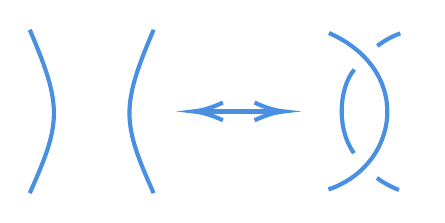
\begin{tikzpicture}[x=0.75pt,y=0.75pt,yscale=-1,xscale=1]
                %uncomment if require: \path (0,82); %set diagram left start at 0, and has height of 82
                
                %Curve Lines [id:da28666373624741825] 
                \draw [color={rgb, 255:red, 74; green, 144; blue, 226 }  ,draw opacity=1 ][line width=1.5]    (231.17,1.01) .. controls (246.9,37.91) and (246.47,45.59) .. (231.17,79.72) ;
                %Curve Lines [id:da6473636293749112] 
                \draw [color={rgb, 255:red, 74; green, 144; blue, 226 }  ,draw opacity=1 ][line width=1.5]    (290.85,1.01) .. controls (275.12,37.91) and (275.54,45.59) .. (290.85,79.72) ;
                
                %Curve Lines [id:da34726741926398463] 
                \draw [color={rgb, 255:red, 74; green, 144; blue, 226 }  ,draw opacity=1 ][line width=1.5]    (375.31,2.56) .. controls (416.46,20.8) and (409.06,66.44) .. (375.08,77.96) ;
                %Curve Lines [id:da9780689263100604] 
                \draw [color={rgb, 255:red, 74; green, 144; blue, 226 }  ,draw opacity=1 ][line width=1.5]    (409.7,2.77) .. controls (405.6,4.17) and (401.2,6.73) .. (398.66,8.86) ;
                %Curve Lines [id:da16670674465631863] 
                \draw [color={rgb, 255:red, 74; green, 144; blue, 226 }  ,draw opacity=1 ][line width=1.5]    (398.43,72.41) .. controls (401.9,74.97) and (406.06,77.1) .. (409.06,78.17) ;
                %Curve Lines [id:da3643115225934235] 
                \draw [color={rgb, 255:red, 74; green, 144; blue, 226 }  ,draw opacity=1 ][line width=1.5]    (387.56,20.16) .. controls (380.4,28.55) and (378.55,48.1) .. (387.33,60.47) ;
                
                %Straight Lines [id:da4458936620449674] 
                \draw [color={rgb, 255:red, 74; green, 144; blue, 226 }  ,draw opacity=1 ][line width=1.5]    (313,40.36) -- (350.7,40.36) ;
                \draw [shift={(353.7,40.36)}, rotate = 180] [color={rgb, 255:red, 74; green, 144; blue, 226 }  ,draw opacity=1 ][line width=1.5]    (14.21,-4.28) .. controls (9.04,-1.82) and (4.3,-0.39) .. (0,0) .. controls (4.3,0.39) and (9.04,1.82) .. (14.21,4.28)   ;
                \draw [shift={(310,40.36)}, rotate = 0] [color={rgb, 255:red, 74; green, 144; blue, 226 }  ,draw opacity=1 ][line width=1.5]    (14.21,-4.28) .. controls (9.04,-1.82) and (4.3,-0.39) .. (0,0) .. controls (4.3,0.39) and (9.04,1.82) .. (14.21,4.28)   ;
        \end{tikzpicture}
        \caption{Reidermeister move of type II}
        \label{fig:ReidermeisterMoveOfTypeII}
\end{figure}
Then according to the definition of the Kauffman bracket, we have:
\begin{equation*}
        \begin{aligned}
                \tikzset{every picture/.style={line width=0.75pt}} %set default line width to 0.75pt        
                \begin{tikzpicture}[x=0.75pt,y=0.75pt,yscale=-1,xscale=1, baseline=(XXXX.south) ]
                        \path (0,83);\path (40.99652099609375,0);\draw    ($(current bounding box.center)+(0,0.3em)$) node [anchor=south] (XXXX) {};
                        %Curve Lines [id:da9604095537894752] 
                        \draw [color={rgb, 255:red, 74; green, 144; blue, 226 }  ,draw opacity=1 ][line width=1.5]    (3.31,4.56) .. controls (44.46,22.8) and (37.06,68.44) .. (3.08,79.96) ;
                        %Curve Lines [id:da44353755004889783] 
                        \draw [color={rgb, 255:red, 74; green, 144; blue, 226 }  ,draw opacity=1 ][line width=1.5]    (37.7,4.77) .. controls (33.6,6.17) and (29.2,8.73) .. (26.66,10.86) ;
                        %Curve Lines [id:da9884546368227021] 
                        \draw [color={rgb, 255:red, 74; green, 144; blue, 226 }  ,draw opacity=1 ][line width=1.5]    (26.43,74.41) .. controls (29.9,76.97) and (34.06,79.1) .. (37.06,80.17) ;
                        %Curve Lines [id:da1642034829302086] 
                        \draw [color={rgb, 255:red, 74; green, 144; blue, 226 }  ,draw opacity=1 ][line width=1.5]    (15.56,22.16) .. controls (8.4,30.55) and (6.55,50.1) .. (15.33,62.47) ;
                \end{tikzpicture}
                & =A\tikzset{every picture/.style={line width=0.75pt}} %set default line width to 0.75pt        
                \begin{tikzpicture}[x=0.75pt,y=0.75pt,yscale=-1,xscale=1, baseline=(XXXX.south) ]
                        \path (0,68);\path (68.99652099609375,0);\draw    ($(current bounding box.center)+(0,0.3em)$) node [anchor=south] (XXXX) {};
                        %Straight Lines [id:da6104518270284445] 
                        \draw [color={rgb, 255:red, 74; green, 144; blue, 226 }  ,draw opacity=1 ][line width=1.5]    (65.7,3.81) -- (3,66.51) ;
                        %Straight Lines [id:da0766348817654059] 
                        \draw [color={rgb, 255:red, 74; green, 144; blue, 226 }  ,draw opacity=1 ][line width=1.5]    (41.56,41.59) -- (66.56,66.59) ;
                        %Straight Lines [id:da42798350857778145] 
                        \draw [color={rgb, 255:red, 74; green, 144; blue, 226 }  ,draw opacity=1 ][line width=1.5]    (3.23,3.25) -- (28.23,28.25) ;
                \end{tikzpicture}
                +A^{-1}\tikzset{every picture/.style={line width=0.75pt}} %set default line width to 0.75pt        
                \begin{tikzpicture}[x=0.75pt,y=0.75pt,yscale=-1,xscale=1, baseline=(XXXX.south) ]
                        \path (0,92);\path (50.99652099609375,0);\draw    ($(current bounding box.center)+(0,0.3em)$) node [anchor=south] (XXXX) {};
                        %Curve Lines [id:da6343061819532925] 
                        \draw [color={rgb, 255:red, 74; green, 144; blue, 226 }  ,draw opacity=1 ][line width=1.5]    (48.86,3.92) .. controls (27.16,14.74) and (22.64,14.45) .. (2.57,3.92) ;
                        %Straight Lines [id:da10138287838463445] 
                        \draw [color={rgb, 255:red, 74; green, 144; blue, 226 }  ,draw opacity=1 ][line width=1.5]    (30.64,71.36) -- (48.82,89.54) ;
                        %Curve Lines [id:da8125503416637623] 
                        \draw [color={rgb, 255:red, 74; green, 144; blue, 226 }  ,draw opacity=1 ][line width=1.5]    (20.95,61.67) .. controls (13.06,53.79) and (8.33,48.34) .. (2.78,43.5) .. controls (2.88,15.63) and (47.22,12.36) .. (48.19,43.9) .. controls (39.59,52.34) and (12.69,78.88) .. (2.61,89.48) ;
                \end{tikzpicture}
                \\
                & =A\left( A\tikzset{every picture/.style={line width=0.75pt}} %set default line width to 0.75pt        
                \begin{tikzpicture}[x=0.75pt,y=0.75pt,yscale=-1,xscale=1, baseline=(XXXX.south) ]
                        \path (0,67);\path (71.98169708251953,0);\draw    ($(current bounding box.center)+(0,0.3em)$) node [anchor=south] (XXXX) {};
                        %Curve Lines [id:da12181300195230782] 
                        \draw [color={rgb, 255:red, 74; green, 144; blue, 226 }  ,draw opacity=1 ][line width=1.5]    (68.81,4.31) .. controls (38.96,19.2) and (32.75,18.79) .. (5.15,4.31) ;
                        %Curve Lines [id:da003208814156384854] 
                        \draw [color={rgb, 255:red, 74; green, 144; blue, 226 }  ,draw opacity=1 ][line width=1.5]    (68.81,60.79) .. controls (38.96,45.9) and (32.75,46.3) .. (5.15,60.79) ;
                \end{tikzpicture}
                +A^{-1}\tikzset{every picture/.style={line width=0.75pt}} %set default line width to 0.75pt        
                \begin{tikzpicture}[x=0.75pt,y=0.75pt,yscale=-1,xscale=1, baseline=(XXXX.south) ]
                        \path (0,68);\path (53.991668701171875,0);\draw    ($(current bounding box.center)+(0,0.3em)$) node [anchor=south] (XXXX) {};
                        %Curve Lines [id:da296212719001264] 
                        \draw [color={rgb, 255:red, 74; green, 144; blue, 226 }  ,draw opacity=1 ][line width=1.5]    (4.17,2.29) .. controls (16.5,31.12) and (16.17,37.12) .. (4.17,63.79) ;
                        %Curve Lines [id:da14704308294878077] 
                        \draw [color={rgb, 255:red, 74; green, 144; blue, 226 }  ,draw opacity=1 ][line width=1.5]    (50.96,2.29) .. controls (38.63,31.12) and (38.96,37.12) .. (50.96,63.79) ;
                \end{tikzpicture}
                \right) +A^{-1}\left( A\tikzset{every picture/.style={line width=0.75pt}} %set default line width to 0.75pt        
                \begin{tikzpicture}[x=0.75pt,y=0.75pt,yscale=-1,xscale=1, baseline=(XXXX.south) ]
                        \path (0,68);\path (58.99652099609375,0);\draw    ($(current bounding box.center)+(0,0.3em)$) node [anchor=south] (XXXX) {};
                        %Curve Lines [id:da912568481834767] 
                        \draw [color={rgb, 255:red, 74; green, 144; blue, 226 }  ,draw opacity=1 ][line width=1.5]    (56.68,2.54) .. controls (31.58,15.06) and (26.36,14.72) .. (3.15,2.54) ;
                        %Curve Lines [id:da17235049610260633] 
                        \draw [color={rgb, 255:red, 74; green, 144; blue, 226 }  ,draw opacity=1 ][line width=1.5]    (56.68,67.17) .. controls (31.58,54.65) and (26.36,54.99) .. (3.15,67.17) ;
                        %Shape: Ellipse [id:dp9280843921436426] 
                        \draw  [color={rgb, 255:red, 74; green, 144; blue, 226 }  ,draw opacity=1 ][line width=1.5]  (15.74,34.85) .. controls (15.74,27.02) and (22.08,20.68) .. (29.91,20.68) .. controls (37.74,20.68) and (44.09,27.02) .. (44.09,34.85) .. controls (44.09,42.68) and (37.74,49.03) .. (29.91,49.03) .. controls (22.08,49.03) and (15.74,42.68) .. (15.74,34.85) -- cycle ;
                \end{tikzpicture}
                +A^{-1}\tikzset{every picture/.style={line width=0.75pt}} %set default line width to 0.75pt        
                \begin{tikzpicture}[x=0.75pt,y=0.75pt,yscale=-1,xscale=1, baseline=(XXXX.south) ]
                        \path (0,67);\path (71.98169708251953,0);\draw    ($(current bounding box.center)+(0,0.3em)$) node [anchor=south] (XXXX) {};
                        %Curve Lines [id:da4627840070580258] 
                        \draw [color={rgb, 255:red, 74; green, 144; blue, 226 }  ,draw opacity=1 ][line width=1.5]    (68.81,4.31) .. controls (38.96,19.2) and (32.75,18.79) .. (5.15,4.31) ;
                        %Curve Lines [id:da7914769351421946] 
                        \draw [color={rgb, 255:red, 74; green, 144; blue, 226 }  ,draw opacity=1 ][line width=1.5]    (68.81,60.79) .. controls (38.96,45.9) and (32.75,46.3) .. (5.15,60.79) ;
                \end{tikzpicture}
                \right)\\
                & =A^{2}\tikzset{every picture/.style={line width=0.75pt}} %set default line width to 0.75pt        
                \begin{tikzpicture}[x=0.75pt,y=0.75pt,yscale=-1,xscale=1, baseline=(XXXX.south) ]
                        \path (0,67);\path (71.98169708251953,0);\draw    ($(current bounding box.center)+(0,0.3em)$) node [anchor=south] (XXXX) {};
                        %Curve Lines [id:da2751841456474464] 
                        \draw [color={rgb, 255:red, 74; green, 144; blue, 226 }  ,draw opacity=1 ][line width=1.5]    (68.81,4.31) .. controls (38.96,19.2) and (32.75,18.79) .. (5.15,4.31) ;
                        %Curve Lines [id:da28927063236750583] 
                        \draw [color={rgb, 255:red, 74; green, 144; blue, 226 }  ,draw opacity=1 ][line width=1.5]    (68.81,60.79) .. controls (38.96,45.9) and (32.75,46.3) .. (5.15,60.79) ;
                \end{tikzpicture}
                +\tikzset{every picture/.style={line width=0.75pt}} %set default line width to 0.75pt        
                \begin{tikzpicture}[x=0.75pt,y=0.75pt,yscale=-1,xscale=1, baseline=(XXXX.south) ]
                        \path (0,68);\path (53.991668701171875,0);\draw    ($(current bounding box.center)+(0,0.3em)$) node [anchor=south] (XXXX) {};
                        %Curve Lines [id:da32898216042375594] 
                        \draw [color={rgb, 255:red, 74; green, 144; blue, 226 }  ,draw opacity=1 ][line width=1.5]    (4.17,2.29) .. controls (16.5,31.12) and (16.17,37.12) .. (4.17,63.79) ;
                        %Curve Lines [id:da2744164658246455] 
                        \draw [color={rgb, 255:red, 74; green, 144; blue, 226 }  ,draw opacity=1 ][line width=1.5]    (50.96,2.29) .. controls (38.63,31.12) and (38.96,37.12) .. (50.96,63.79) ;
                \end{tikzpicture}
                +d\tikzset{every picture/.style={line width=0.75pt}} %set default line width to 0.75pt        
                \begin{tikzpicture}[x=0.75pt,y=0.75pt,yscale=-1,xscale=1, baseline=(XXXX.south) ]
                        \path (0,67);\path (71.98169708251953,0);\draw    ($(current bounding box.center)+(0,0.3em)$) node [anchor=south] (XXXX) {};
                        %Curve Lines [id:da6870558472651833] 
                        \draw [color={rgb, 255:red, 74; green, 144; blue, 226 }  ,draw opacity=1 ][line width=1.5]    (68.81,4.31) .. controls (38.96,19.2) and (32.75,18.79) .. (5.15,4.31) ;
                        %Curve Lines [id:da13357681707506375] 
                        \draw [color={rgb, 255:red, 74; green, 144; blue, 226 }  ,draw opacity=1 ][line width=1.5]    (68.81,60.79) .. controls (38.96,45.9) and (32.75,46.3) .. (5.15,60.79) ;
                \end{tikzpicture}
                +A^{-2}\tikzset{every picture/.style={line width=0.75pt}} %set default line width to 0.75pt        
                \begin{tikzpicture}[x=0.75pt,y=0.75pt,yscale=-1,xscale=1, baseline=(XXXX.south) ]
                        \path (0,67);\path (71.98169708251953,0);\draw    ($(current bounding box.center)+(0,0.3em)$) node [anchor=south] (XXXX) {};
                        %Curve Lines [id:da8617051673767433] 
                        \draw [color={rgb, 255:red, 74; green, 144; blue, 226 }  ,draw opacity=1 ][line width=1.5]    (68.81,4.31) .. controls (38.96,19.2) and (32.75,18.79) .. (5.15,4.31) ;
                        %Curve Lines [id:da5303437875908261] 
                        \draw [color={rgb, 255:red, 74; green, 144; blue, 226 }  ,draw opacity=1 ][line width=1.5]    (68.81,60.79) .. controls (38.96,45.9) and (32.75,46.3) .. (5.15,60.79) ;
                \end{tikzpicture}
                \\
                & =\tikzset{every picture/.style={line width=0.75pt}} %set default line width to 0.75pt        
                \begin{tikzpicture}[x=0.75pt,y=0.75pt,yscale=-1,xscale=1, baseline=(XXXX.south) ]
                        \path (0,68);\path (53.991668701171875,0);\draw    ($(current bounding box.center)+(0,0.3em)$) node [anchor=south] (XXXX) {};
                        %Curve Lines [id:da9892583999632016] 
                        \draw [color={rgb, 255:red, 74; green, 144; blue, 226 }  ,draw opacity=1 ][line width=1.5]    (4.17,2.29) .. controls (16.5,31.12) and (16.17,37.12) .. (4.17,63.79) ;
                        %Curve Lines [id:da9019420104276974] 
                        \draw [color={rgb, 255:red, 74; green, 144; blue, 226 }  ,draw opacity=1 ][line width=1.5]    (50.96,2.29) .. controls (38.63,31.12) and (38.96,37.12) .. (50.96,63.79) ;
                \end{tikzpicture}
                .
        \end{aligned}
\end{equation*}
In the last line we use $d=-A^{2} -A^{-2}$. Now we can see type II is invariant. 

(b) The Reidermeister move of type III is given by Fig.\ref{fig:ReidermeisterMoveOfTypeIII}.
\begin{figure}[h!]
        \centering
        \tikzset{every picture/.style={line width=0.75pt}} %set default line width to 0.75pt        
        
        \begin{tikzpicture}[x=0.75pt,y=0.75pt,yscale=-1,xscale=1]
                %uncomment if require: \path (0,83); %set diagram left start at 0, and has height of 83
                
                %Straight Lines [id:da11950785204529102] 
                \draw [color={rgb, 255:red, 74; green, 144; blue, 226 }  ,draw opacity=1 ][line width=1.5]    (313,40.77) -- (350.7,40.77) ;
                \draw [shift={(353.7,40.77)}, rotate = 180] [color={rgb, 255:red, 74; green, 144; blue, 226 }  ,draw opacity=1 ][line width=1.5]    (14.21,-4.28) .. controls (9.04,-1.82) and (4.3,-0.39) .. (0,0) .. controls (4.3,0.39) and (9.04,1.82) .. (14.21,4.28)   ;
                \draw [shift={(310,40.77)}, rotate = 0] [color={rgb, 255:red, 74; green, 144; blue, 226 }  ,draw opacity=1 ][line width=1.5]    (14.21,-4.28) .. controls (9.04,-1.82) and (4.3,-0.39) .. (0,0) .. controls (4.3,0.39) and (9.04,1.82) .. (14.21,4.28)   ;
                %Straight Lines [id:da8207765534905693] 
                \draw [color={rgb, 255:red, 74; green, 144; blue, 226 }  ,draw opacity=1 ][line width=1.5]    (229.76,4.84) -- (302.61,77.69) ;
                %Straight Lines [id:da43977309937961295] 
                \draw [color={rgb, 255:red, 74; green, 144; blue, 226 }  ,draw opacity=1 ][line width=1.5]    (273.65,32.88) -- (302.7,3.84) ;
                %Straight Lines [id:da7291965597075933] 
                \draw [color={rgb, 255:red, 74; green, 144; blue, 226 }  ,draw opacity=1 ][line width=1.5]    (229.11,77.43) -- (258.16,48.38) ;
                %Straight Lines [id:da9127752946580543] 
                \draw [color={rgb, 255:red, 74; green, 144; blue, 226 }  ,draw opacity=1 ][line width=1.5]    (251.18,4.66) -- (251.18,19.4) ;
                %Straight Lines [id:da5580787674820835] 
                \draw [color={rgb, 255:red, 74; green, 144; blue, 226 }  ,draw opacity=1 ][line width=1.5]    (251.18,32.2) -- (251.18,47.51) ;
                %Straight Lines [id:da5788807019103526] 
                \draw [color={rgb, 255:red, 74; green, 144; blue, 226 }  ,draw opacity=1 ][line width=1.5]    (251.18,61.42) -- (251.18,76.72) ;
                
                %Straight Lines [id:da1822021649397716] 
                \draw [color={rgb, 255:red, 74; green, 144; blue, 226 }  ,draw opacity=1 ][line width=1.5]    (359.42,5.16) -- (431.61,77.36) ;
                %Straight Lines [id:da719661142881121] 
                \draw [color={rgb, 255:red, 74; green, 144; blue, 226 }  ,draw opacity=1 ][line width=1.5]    (398.68,37.19) -- (431.7,4.17) ;
                %Straight Lines [id:da0823586599622459] 
                \draw [color={rgb, 255:red, 74; green, 144; blue, 226 }  ,draw opacity=1 ][line width=1.5]    (358.78,77.09) -- (391.3,44.58) ;
                %Straight Lines [id:da8525034743711262] 
                \draw [color={rgb, 255:red, 74; green, 144; blue, 226 }  ,draw opacity=1 ][line width=1.5]    (409.01,4.98) -- (409.01,19.6) ;
                %Straight Lines [id:da246160857461047] 
                \draw [color={rgb, 255:red, 74; green, 144; blue, 226 }  ,draw opacity=1 ][line width=1.5]    (409.01,32.28) -- (409.01,47.45) ;
                %Straight Lines [id:da5380394964109403] 
                \draw [color={rgb, 255:red, 74; green, 144; blue, 226 }  ,draw opacity=1 ][line width=1.5]    (409.01,61.23) -- (409.01,76.4) ;
        \end{tikzpicture}
        \caption{Reidermeister move of type III}
        \label{fig:ReidermeisterMoveOfTypeIII}
\end{figure}
Then according to the definition of the Kauffman bracket, we have:

\begin{align*}
                \tikzset{every picture/.style={line width=0.75pt}} %set default line width to 0.75pt        
                \begin{tikzpicture}[x=0.75pt,y=0.75pt,yscale=-1,xscale=1, baseline=(XXXX.south) ]
                        \path (0,79);\path (76.99652099609375,0);\draw    ($(current bounding box.center)+(0,0.3em)$) node [anchor=south] (XXXX) {};
                        %Straight Lines [id:da5322048377507285] 
                        \draw [color={rgb, 255:red, 74; green, 144; blue, 226 }  ,draw opacity=1 ][line width=1.5]    (2.76,3.84) -- (75.61,76.69) ;
                        %Straight Lines [id:da2834370641983299] 
                        \draw [color={rgb, 255:red, 74; green, 144; blue, 226 }  ,draw opacity=1 ][line width=1.5]    (46.65,31.88) -- (75.7,2.84) ;
                        %Straight Lines [id:da7335835078220603] 
                        \draw [color={rgb, 255:red, 74; green, 144; blue, 226 }  ,draw opacity=1 ][line width=1.5]    (2.11,76.43) -- (31.16,47.38) ;
                        %Straight Lines [id:da6290897514246225] 
                        \draw [color={rgb, 255:red, 74; green, 144; blue, 226 }  ,draw opacity=1 ][line width=1.5]    (24.18,3.66) -- (24.18,18.4) ;
                        %Straight Lines [id:da7855778727017275] 
                        \draw [color={rgb, 255:red, 74; green, 144; blue, 226 }  ,draw opacity=1 ][line width=1.5]    (24.18,31.2) -- (24.18,46.51) ;
                        %Straight Lines [id:da40285349600704823] 
                        \draw [color={rgb, 255:red, 74; green, 144; blue, 226 }  ,draw opacity=1 ][line width=1.5]    (24.18,60.42) -- (24.18,75.72) ;
                \end{tikzpicture}
                & =A\tikzset{every picture/.style={line width=0.75pt}} %set default line width to 0.75pt        
                \begin{tikzpicture}[x=0.75pt,y=0.75pt,yscale=-1,xscale=1, baseline=(XXXX.south) ]
                        \path (0,79);\path (97.99652099609375,0);\draw    ($(current bounding box.center)+(0,0.3em)$) node [anchor=south] (XXXX) {};
                        %Straight Lines [id:da651734203263048] 
                        \draw [color={rgb, 255:red, 74; green, 144; blue, 226 }  ,draw opacity=1 ][line width=1.5]    (22.94,1.73) -- (97.13,75.92) ;
                        %Straight Lines [id:da9822862230824239] 
                        \draw [color={rgb, 255:red, 74; green, 144; blue, 226 }  ,draw opacity=1 ][line width=1.5]    (58.66,25.97) -- (82,2.63) ;
                        %Straight Lines [id:da5738361847067126] 
                        \draw [color={rgb, 255:red, 74; green, 144; blue, 226 }  ,draw opacity=1 ][line width=1.5]    (8.71,76.73) -- (46.16,39.29) ;
                        %Straight Lines [id:da651347852864083] 
                        \draw [color={rgb, 255:red, 74; green, 144; blue, 226 }  ,draw opacity=1 ][line width=1.5]    (37.54,61.48) -- (52.8,76.73) ;
                        %Straight Lines [id:da16594256373987704] 
                        \draw [color={rgb, 255:red, 74; green, 144; blue, 226 }  ,draw opacity=1 ][line width=1.5]    (3.89,29.45) -- (22.64,48.2) ;
                \end{tikzpicture}
                +A^{-1}\tikzset{every picture/.style={line width=0.75pt}} %set default line width to 0.75pt        
                \begin{tikzpicture}[x=0.75pt,y=0.75pt,yscale=-1,xscale=1, baseline=(XXXX.south) ]
                        \path (0,81);\path (79.99413299560547,0);\draw    ($(current bounding box.center)+(0,0.3em)$) node [anchor=south] (XXXX) {};
                        %Curve Lines [id:da9862043434565733] 
                        \draw [color={rgb, 255:red, 74; green, 144; blue, 226 }  ,draw opacity=1 ][line width=1.5]    (62.72,2.31) .. controls (37.09,15.09) and (31.75,14.75) .. (8.04,2.31) ;
                        %Straight Lines [id:da7232272884844684] 
                        \draw [color={rgb, 255:red, 74; green, 144; blue, 226 }  ,draw opacity=1 ][line width=1.5]    (47.49,38.48) -- (66.18,19.79) ;
                        %Straight Lines [id:da5625150004968165] 
                        \draw [color={rgb, 255:red, 74; green, 144; blue, 226 }  ,draw opacity=1 ][line width=1.5]    (7.51,79.11) -- (37.49,49.14) ;
                        %Straight Lines [id:da4800775441178744] 
                        \draw [color={rgb, 255:red, 74; green, 144; blue, 226 }  ,draw opacity=1 ][line width=1.5]    (30.59,66.9) -- (42.81,79.11) ;
                        %Curve Lines [id:da8772854853652521] 
                        \draw [color={rgb, 255:red, 74; green, 144; blue, 226 }  ,draw opacity=1 ][line width=1.5]    (18.66,56.27) .. controls (0.27,39.31) and (-2.34,26.91) .. (5.49,21.03) .. controls (13.32,15.16) and (21.8,22.34) .. (78.29,78.46) ;
                \end{tikzpicture}
                \\
                & =A\left( A\tikzset{every picture/.style={line width=0.75pt}} %set default line width to 0.75pt        
                \begin{tikzpicture}[x=0.75pt,y=0.75pt,yscale=-1,xscale=1, baseline=(XXXX.south) ]
                        \path (0,74);\path (74.99585723876953,0);\draw    ($(current bounding box.center)+(0,0.3em)$) node [anchor=south] (XXXX) {};
                        %Straight Lines [id:da9591344309737191] 
                        \draw [color={rgb, 255:red, 74; green, 144; blue, 226 }  ,draw opacity=1 ][line width=1.5]    (4.57,4.74) -- (70.04,48.7) ;
                        %Straight Lines [id:da22448626545323047] 
                        \draw [color={rgb, 255:red, 74; green, 144; blue, 226 }  ,draw opacity=1 ][line width=1.5]    (44.02,21.66) -- (70.12,4.14) ;
                        %Straight Lines [id:da452032535930315] 
                        \draw [color={rgb, 255:red, 74; green, 144; blue, 226 }  ,draw opacity=1 ][line width=1.5]    (3.99,48.54) -- (30.09,31.01) ;
                        %Curve Lines [id:da3238575571012392] 
                        \draw [color={rgb, 255:red, 74; green, 144; blue, 226 }  ,draw opacity=1 ][line width=1.5]    (68.89,69) .. controls (39.04,54.11) and (32.83,54.51) .. (5.22,69) ;
                \end{tikzpicture}
                +A^{-1}\tikzset{every picture/.style={line width=0.75pt}} %set default line width to 0.75pt        
                \begin{tikzpicture}[x=0.75pt,y=0.75pt,yscale=-1,xscale=1, baseline=(XXXX.south) ]
                        \path (0,64);\path (61.991004943847656,0);\draw    ($(current bounding box.center)+(0,0.3em)$) node [anchor=south] (XXXX) {};
                        %Straight Lines [id:da4597054660712325] 
                        \draw [color={rgb, 255:red, 74; green, 144; blue, 226 }  ,draw opacity=1 ][line width=1.5]    (17.45,4.43) -- (56.2,63.52) ;
                        %Straight Lines [id:da9036592905897192] 
                        \draw [color={rgb, 255:red, 74; green, 144; blue, 226 }  ,draw opacity=1 ][line width=1.5]    (40.8,27.18) -- (56.24,3.61) ;
                        %Straight Lines [id:da16547855392481936] 
                        \draw [color={rgb, 255:red, 74; green, 144; blue, 226 }  ,draw opacity=1 ][line width=1.5]    (17.11,63.31) -- (32.56,39.74) ;
                        %Curve Lines [id:da9241917289860497] 
                        \draw [color={rgb, 255:red, 74; green, 144; blue, 226 }  ,draw opacity=1 ][line width=1.5]    (2.17,2.82) .. controls (14.5,31.65) and (14.17,37.65) .. (2.17,64.32) ;
                \end{tikzpicture}
                \right) +A^{-1}\left( A\tikzset{every picture/.style={line width=0.75pt}} %set default line width to 0.75pt        
                \begin{tikzpicture}[x=0.75pt,y=0.75pt,yscale=-1,xscale=1, baseline=(XXXX.south) ]
                        \path (0,67);\path (65.99652099609375,0);\draw    ($(current bounding box.center)+(0,0.3em)$) node [anchor=south] (XXXX) {};
                        %Curve Lines [id:da3283442283468585] 
                        \draw [color={rgb, 255:red, 74; green, 144; blue, 226 }  ,draw opacity=1 ][line width=1.5]    (66,2.52) .. controls (36.15,17.41) and (29.94,17) .. (2.33,2.52) ;
                        %Curve Lines [id:da08588422248637961] 
                        \draw [color={rgb, 255:red, 74; green, 144; blue, 226 }  ,draw opacity=1 ][line width=1.5]    (66,64) .. controls (36.15,49.11) and (29.94,49.51) .. (2.33,64) ;
                        %Curve Lines [id:da9555444507529145] 
                        \draw [color={rgb, 255:red, 74; green, 144; blue, 226 }  ,draw opacity=1 ][line width=1.5]    (40.2,33.6) .. controls (19.2,47.58) and (2.06,47.31) .. (2.13,33.44) .. controls (2.2,19.58) and (50.2,24.6) .. (66.2,41.6) ;
                        %Curve Lines [id:da2724960587777081] 
                        \draw [color={rgb, 255:red, 74; green, 144; blue, 226 }  ,draw opacity=1 ][line width=1.5]    (47.2,26.6) .. controls (53.67,22.9) and (58.67,20.23) .. (65.2,20.6) ;
                \end{tikzpicture}
                +A^{-1}\tikzset{every picture/.style={line width=0.75pt}} %set default line width to 0.75pt        
                \begin{tikzpicture}[x=0.75pt,y=0.75pt,yscale=-1,xscale=1, baseline=(XXXX.south) ]
                        \path (0,74);\path (74.99585723876953,0);\draw    ($(current bounding box.center)+(0,0.3em)$) node [anchor=south] (XXXX) {};
                        %Straight Lines [id:da9065450436189566] 
                        \draw [color={rgb, 255:red, 74; green, 144; blue, 226 }  ,draw opacity=1 ][line width=1.5]    (4.59,20.23) -- (72.71,69.05) ;
                        %Straight Lines [id:da4804591340207396] 
                        \draw [color={rgb, 255:red, 74; green, 144; blue, 226 }  ,draw opacity=1 ][line width=1.5]    (45.63,39.02) -- (72.79,19.56) ;
                        %Straight Lines [id:da3666760694217881] 
                        \draw [color={rgb, 255:red, 74; green, 144; blue, 226 }  ,draw opacity=1 ][line width=1.5]    (3.99,68.87) -- (31.15,49.4) ;
                        %Curve Lines [id:da7794924828593213] 
                        \draw [color={rgb, 255:red, 74; green, 144; blue, 226 }  ,draw opacity=1 ][line width=1.5]    (71.62,5.31) .. controls (40.57,21.84) and (34.1,21.4) .. (5.38,5.31) ;
                \end{tikzpicture}
                \right)\\
                & =A^{2}\tikzset{every picture/.style={line width=0.75pt}} %set default line width to 0.75pt        
                \begin{tikzpicture}[x=0.75pt,y=0.75pt,yscale=-1,xscale=1, baseline=(XXXX.south) ]
                        \path (0,74);\path (74.99585723876953,0);\draw    ($(current bounding box.center)+(0,0.3em)$) node [anchor=south] (XXXX) {};
                        %Straight Lines [id:da6841403382603282] 
                        \draw [color={rgb, 255:red, 74; green, 144; blue, 226 }  ,draw opacity=1 ][line width=1.5]    (4.57,4.74) -- (70.04,48.7) ;
                        %Straight Lines [id:da8167315388208278] 
                        \draw [color={rgb, 255:red, 74; green, 144; blue, 226 }  ,draw opacity=1 ][line width=1.5]    (44.02,21.66) -- (70.12,4.14) ;
                        %Straight Lines [id:da7860921281606539] 
                        \draw [color={rgb, 255:red, 74; green, 144; blue, 226 }  ,draw opacity=1 ][line width=1.5]    (3.99,48.54) -- (30.09,31.01) ;
                        %Curve Lines [id:da45872431121640656] 
                        \draw [color={rgb, 255:red, 74; green, 144; blue, 226 }  ,draw opacity=1 ][line width=1.5]    (68.89,69) .. controls (39.04,54.11) and (32.83,54.51) .. (5.22,69) ;
                \end{tikzpicture}
                +\tikzset{every picture/.style={line width=0.75pt}} %set default line width to 0.75pt        
                \begin{tikzpicture}[x=0.75pt,y=0.75pt,yscale=-1,xscale=1, baseline=(XXXX.south) ]
                        \path (0,64);\path (61.991004943847656,0);\draw    ($(current bounding box.center)+(0,0.3em)$) node [anchor=south] (XXXX) {};
                        %Straight Lines [id:da5762679515989089] 
                        \draw [color={rgb, 255:red, 74; green, 144; blue, 226 }  ,draw opacity=1 ][line width=1.5]    (17.45,4.43) -- (56.2,63.52) ;
                        %Straight Lines [id:da5946601466661465] 
                        \draw [color={rgb, 255:red, 74; green, 144; blue, 226 }  ,draw opacity=1 ][line width=1.5]    (40.8,27.18) -- (56.24,3.61) ;
                        %Straight Lines [id:da3025487991076059] 
                        \draw [color={rgb, 255:red, 74; green, 144; blue, 226 }  ,draw opacity=1 ][line width=1.5]    (17.11,63.31) -- (32.56,39.74) ;
                        %Curve Lines [id:da8120924358614992] 
                        \draw [color={rgb, 255:red, 74; green, 144; blue, 226 }  ,draw opacity=1 ][line width=1.5]    (2.17,2.82) .. controls (14.5,31.65) and (14.17,37.65) .. (2.17,64.32) ;
                \end{tikzpicture}
                +\tikzset{every picture/.style={line width=0.75pt}} %set default line width to 0.75pt        
                \begin{tikzpicture}[x=0.75pt,y=0.75pt,yscale=-1,xscale=1, baseline=(XXXX.south) ]
                        \path (0,67);\path (65.99652099609375,0);\draw    ($(current bounding box.center)+(0,0.3em)$) node [anchor=south] (XXXX) {};
                        %Curve Lines [id:da8066902275465357] 
                        \draw [color={rgb, 255:red, 74; green, 144; blue, 226 }  ,draw opacity=1 ][line width=1.5]    (66,2.52) .. controls (36.15,17.41) and (29.94,17) .. (2.33,2.52) ;
                        %Curve Lines [id:da5803036714274801] 
                        \draw [color={rgb, 255:red, 74; green, 144; blue, 226 }  ,draw opacity=1 ][line width=1.5]    (66,64) .. controls (36.15,49.11) and (29.94,49.51) .. (2.33,64) ;
                        %Curve Lines [id:da1465258396067759] 
                        \draw [color={rgb, 255:red, 74; green, 144; blue, 226 }  ,draw opacity=1 ][line width=1.5]    (40.2,33.6) .. controls (19.2,47.58) and (2.06,47.31) .. (2.13,33.44) .. controls (2.2,19.58) and (50.2,24.6) .. (66.2,41.6) ;
                        %Curve Lines [id:da7828362623581651] 
                        \draw [color={rgb, 255:red, 74; green, 144; blue, 226 }  ,draw opacity=1 ][line width=1.5]    (47.2,26.6) .. controls (54.2,21.6) and (58.2,19.6) .. (65.2,20.6) ;
                \end{tikzpicture}
                +A^{-2}\tikzset{every picture/.style={line width=0.75pt}} %set default line width to 0.75pt        
                \begin{tikzpicture}[x=0.75pt,y=0.75pt,yscale=-1,xscale=1, baseline=(XXXX.south) ]
                        \path (0,74);\path (74.99585723876953,0);\draw    ($(current bounding box.center)+(0,0.3em)$) node [anchor=south] (XXXX) {};
                        %Straight Lines [id:da6133566330648923] 
                        \draw [color={rgb, 255:red, 74; green, 144; blue, 226 }  ,draw opacity=1 ][line width=1.5]    (4.59,20.23) -- (72.71,69.05) ;
                        %Straight Lines [id:da27516495259545626] 
                        \draw [color={rgb, 255:red, 74; green, 144; blue, 226 }  ,draw opacity=1 ][line width=1.5]    (45.63,39.02) -- (72.79,19.56) ;
                        %Straight Lines [id:da44400211184932603] 
                        \draw [color={rgb, 255:red, 74; green, 144; blue, 226 }  ,draw opacity=1 ][line width=1.5]    (3.99,68.87) -- (31.15,49.4) ;
                        %Curve Lines [id:da5237433546266892] 
                        \draw [color={rgb, 255:red, 74; green, 144; blue, 226 }  ,draw opacity=1 ][line width=1.5]    (71.62,5.31) .. controls (40.57,21.84) and (34.1,21.4) .. (5.38,5.31) ;
                \end{tikzpicture}
                .
\end{align*}

Similarly, we can also work out that
\begin{equation*}
        \tikzset{every picture/.style={line width=0.75pt}} %set default line width to 0.75pt        
        \begin{tikzpicture}[x=0.75pt,y=0.75pt,yscale=-1,xscale=1, baseline=(XXXX.south) ]
                \path (0,79);\path (76.99652099609375,0);\draw    ($(current bounding box.center)+(0,0.3em)$) node [anchor=south] (XXXX) {};
                %Straight Lines [id:da4456215523076539] 
                \draw [color={rgb, 255:red, 74; green, 144; blue, 226 }  ,draw opacity=1 ][line width=1.5]    (3.42,6.16) -- (75.61,78.36) ;
                %Straight Lines [id:da24465539629543986] 
                \draw [color={rgb, 255:red, 74; green, 144; blue, 226 }  ,draw opacity=1 ][line width=1.5]    (42.68,38.19) -- (75.7,5.17) ;
                %Straight Lines [id:da21746736537565248] 
                \draw [color={rgb, 255:red, 74; green, 144; blue, 226 }  ,draw opacity=1 ][line width=1.5]    (2.78,78.09) -- (35.3,45.58) ;
                %Straight Lines [id:da37125615310092086] 
                \draw [color={rgb, 255:red, 74; green, 144; blue, 226 }  ,draw opacity=1 ][line width=1.5]    (53.01,5.98) -- (53.01,20.6) ;
                %Straight Lines [id:da22315148334215507] 
                \draw [color={rgb, 255:red, 74; green, 144; blue, 226 }  ,draw opacity=1 ][line width=1.5]    (53.01,33.28) -- (53.01,48.45) ;
                %Straight Lines [id:da13239005571577134] 
                \draw [color={rgb, 255:red, 74; green, 144; blue, 226 }  ,draw opacity=1 ][line width=1.5]    (53.01,62.23) -- (53.01,77.4) ;
        \end{tikzpicture}
        =A^{2}\tikzset{every picture/.style={line width=0.75pt}} %set default line width to 0.75pt        
        \begin{tikzpicture}[x=0.75pt,y=0.75pt,yscale=-1,xscale=1, baseline=(XXXX.south) ]
                \path (0,74);\path (74.99585723876953,0);\draw    ($(current bounding box.center)+(0,0.3em)$) node [anchor=south] (XXXX) {};
                %Straight Lines [id:da4709299158208502] 
                \draw [color={rgb, 255:red, 74; green, 144; blue, 226 }  ,draw opacity=1 ][line width=1.5]    (4.59,20.23) -- (72.71,69.05) ;
                %Straight Lines [id:da7368811371103137] 
                \draw [color={rgb, 255:red, 74; green, 144; blue, 226 }  ,draw opacity=1 ][line width=1.5]    (45.63,39.02) -- (72.79,19.56) ;
                %Straight Lines [id:da9184258204030906] 
                \draw [color={rgb, 255:red, 74; green, 144; blue, 226 }  ,draw opacity=1 ][line width=1.5]    (3.99,68.87) -- (31.15,49.4) ;
                %Curve Lines [id:da29963768788172396] 
                \draw [color={rgb, 255:red, 74; green, 144; blue, 226 }  ,draw opacity=1 ][line width=1.5]    (71.62,5.31) .. controls (40.57,21.84) and (34.1,21.4) .. (5.38,5.31) ;
        \end{tikzpicture}
        +\tikzset{every picture/.style={line width=0.75pt}} %set default line width to 0.75pt        
        \begin{tikzpicture}[x=0.75pt,y=0.75pt,yscale=-1,xscale=1, baseline=(XXXX.south) ]
                \path (0,67);\path (69.9926528930664,0);\draw    ($(current bounding box.center)+(0,0.3em)$) node [anchor=south] (XXXX) {};
                %Curve Lines [id:da5933305220930818] 
                \draw [color={rgb, 255:red, 74; green, 144; blue, 226 }  ,draw opacity=1 ][line width=1.5]    (2.33,2.52) .. controls (32.18,17.41) and (38.39,17) .. (66,2.52) ;
                %Curve Lines [id:da5132826295408173] 
                \draw [color={rgb, 255:red, 74; green, 144; blue, 226 }  ,draw opacity=1 ][line width=1.5]    (2.33,64) .. controls (32.18,49.11) and (38.39,49.51) .. (66,64) ;
                %Curve Lines [id:da665990401146316] 
                \draw [color={rgb, 255:red, 74; green, 144; blue, 226 }  ,draw opacity=1 ][line width=1.5]    (28.13,30.08) .. controls (49.13,16.09) and (66.27,16.37) .. (66.2,30.23) .. controls (66.13,44.09) and (21.58,38.82) .. (2.13,22.08) ;
                %Curve Lines [id:da9402553759728991] 
                \draw [color={rgb, 255:red, 74; green, 144; blue, 226 }  ,draw opacity=1 ][line width=1.5]    (19.29,36.82) .. controls (15.34,38.56) and (7.58,40.54) .. (3.01,43.96) ;
        \end{tikzpicture}
        +\tikzset{every picture/.style={line width=0.75pt}} %set default line width to 0.75pt        
        \begin{tikzpicture}[x=0.75pt,y=0.75pt,yscale=-1,xscale=1, baseline=(XXXX.south) ]
                \path (0,66);\path (61.991004943847656,0);\draw    ($(current bounding box.center)+(0,0.3em)$) node [anchor=south] (XXXX) {};
                %Straight Lines [id:da23107196473023173] 
                \draw [color={rgb, 255:red, 74; green, 144; blue, 226 }  ,draw opacity=1 ][line width=1.5]    (40.96,4.43) -- (2.22,63.52) ;
                %Straight Lines [id:da23002614456462078] 
                \draw [color={rgb, 255:red, 74; green, 144; blue, 226 }  ,draw opacity=1 ][line width=1.5]    (17.62,27.18) -- (2.17,3.61) ;
                %Straight Lines [id:da6553195295972762] 
                \draw [color={rgb, 255:red, 74; green, 144; blue, 226 }  ,draw opacity=1 ][line width=1.5]    (41.3,63.31) -- (25.85,39.74) ;
                %Curve Lines [id:da5022934803705121] 
                \draw [color={rgb, 255:red, 74; green, 144; blue, 226 }  ,draw opacity=1 ][line width=1.5]    (56.24,2.82) .. controls (43.91,31.65) and (44.24,37.65) .. (56.24,64.32) ;
        \end{tikzpicture}
        +A^{-2}\tikzset{every picture/.style={line width=0.75pt}} %set default line width to 0.75pt        
        \begin{tikzpicture}[x=0.75pt,y=0.75pt,yscale=-1,xscale=1, baseline=(XXXX.south) ]
                \path (0,74);\path (74.99585723876953,0);\draw    ($(current bounding box.center)+(0,0.3em)$) node [anchor=south] (XXXX) {};
                %Straight Lines [id:da38554268799622116] 
                \draw [color={rgb, 255:red, 74; green, 144; blue, 226 }  ,draw opacity=1 ][line width=1.5]    (4.57,4.74) -- (70.04,48.7) ;
                %Straight Lines [id:da12495382628350904] 
                \draw [color={rgb, 255:red, 74; green, 144; blue, 226 }  ,draw opacity=1 ][line width=1.5]    (44.02,21.66) -- (70.12,4.14) ;
                %Straight Lines [id:da8665687593626803] 
                \draw [color={rgb, 255:red, 74; green, 144; blue, 226 }  ,draw opacity=1 ][line width=1.5]    (3.99,48.54) -- (30.09,31.01) ;
                %Curve Lines [id:da07618675458629243] 
                \draw [color={rgb, 255:red, 74; green, 144; blue, 226 }  ,draw opacity=1 ][line width=1.5]    (68.89,69) .. controls (39.04,54.11) and (32.83,54.51) .. (5.22,69) ;
        \end{tikzpicture}
        .
\end{equation*}
If we expand, we will find
\begin{equation*}
        \tikzset{every picture/.style={line width=0.75pt}} %set default line width to 0.75pt        
        \begin{tikzpicture}[x=0.75pt,y=0.75pt,yscale=-1,xscale=1, baseline=(XXXX.south) ]
                \path (0,74);\path (74.99585723876953,0);\draw    ($(current bounding box.center)+(0,0.3em)$) node [anchor=south] (XXXX) {};
                %Straight Lines [id:da13237460150950908] 
                \draw [color={rgb, 255:red, 74; green, 144; blue, 226 }  ,draw opacity=1 ][line width=1.5]    (4.59,20.23) -- (72.71,69.05) ;
                %Straight Lines [id:da5446181227917517] 
                \draw [color={rgb, 255:red, 74; green, 144; blue, 226 }  ,draw opacity=1 ][line width=1.5]    (45.63,39.02) -- (72.79,19.56) ;
                %Straight Lines [id:da4076692773124668] 
                \draw [color={rgb, 255:red, 74; green, 144; blue, 226 }  ,draw opacity=1 ][line width=1.5]    (3.99,68.87) -- (31.15,49.4) ;
                %Curve Lines [id:da785956879155703] 
                \draw [color={rgb, 255:red, 74; green, 144; blue, 226 }  ,draw opacity=1 ][line width=1.5]    (71.62,5.31) .. controls (40.57,21.84) and (34.1,21.4) .. (5.38,5.31) ;
        \end{tikzpicture}
        =\tikzset{every picture/.style={line width=0.75pt}} %set default line width to 0.75pt        
        \begin{tikzpicture}[x=0.75pt,y=0.75pt,yscale=-1,xscale=1, baseline=(XXXX.south) ]
                \path (0,74);\path (74.99585723876953,0);\draw    ($(current bounding box.center)+(0,0.3em)$) node [anchor=south] (XXXX) {};
                %Straight Lines [id:da1636310386009494] 
                \draw [color={rgb, 255:red, 74; green, 144; blue, 226 }  ,draw opacity=1 ][line width=1.5]    (4.57,4.74) -- (70.04,48.7) ;
                %Straight Lines [id:da17168608002947305] 
                \draw [color={rgb, 255:red, 74; green, 144; blue, 226 }  ,draw opacity=1 ][line width=1.5]    (44.02,21.66) -- (70.12,4.14) ;
                %Straight Lines [id:da30205015058719664] 
                \draw [color={rgb, 255:red, 74; green, 144; blue, 226 }  ,draw opacity=1 ][line width=1.5]    (3.99,48.54) -- (30.09,31.01) ;
                %Curve Lines [id:da4524775843403255] 
                \draw [color={rgb, 255:red, 74; green, 144; blue, 226 }  ,draw opacity=1 ][line width=1.5]    (68.89,69) .. controls (39.04,54.11) and (32.83,54.51) .. (5.22,69) ;
        \end{tikzpicture}
\end{equation*}
trivially and
\begin{equation*}
        \tikzset{every picture/.style={line width=0.75pt}} %set default line width to 0.75pt        
        \begin{tikzpicture}[x=0.75pt,y=0.75pt,yscale=-1,xscale=1, baseline=(XXXX.south) ]
                \path (0,67);\path (65.99652099609375,0);\draw    ($(current bounding box.center)+(0,0.3em)$) node [anchor=south] (XXXX) {};
                %Curve Lines [id:da6501140268228529] 
                \draw [color={rgb, 255:red, 74; green, 144; blue, 226 }  ,draw opacity=1 ][line width=1.5]    (66,2.52) .. controls (36.15,17.41) and (29.94,17) .. (2.33,2.52) ;
                %Curve Lines [id:da6914469004290484] 
                \draw [color={rgb, 255:red, 74; green, 144; blue, 226 }  ,draw opacity=1 ][line width=1.5]    (66,64) .. controls (36.15,49.11) and (29.94,49.51) .. (2.33,64) ;
                %Curve Lines [id:da09499828302410296] 
                \draw [color={rgb, 255:red, 74; green, 144; blue, 226 }  ,draw opacity=1 ][line width=1.5]    (40.2,33.6) .. controls (19.2,47.58) and (2.06,47.31) .. (2.13,33.44) .. controls (2.2,19.58) and (50.2,24.6) .. (66.2,41.6) ;
                %Curve Lines [id:da6473588123232106] 
                \draw [color={rgb, 255:red, 74; green, 144; blue, 226 }  ,draw opacity=1 ][line width=1.5]    (47.2,26.6) .. controls (54.2,21.6) and (58.2,19.6) .. (65.2,20.6) ;
        \end{tikzpicture}
        =\tikzset{every picture/.style={line width=0.75pt}} %set default line width to 0.75pt        
        \begin{tikzpicture}[x=0.75pt,y=0.75pt,yscale=-1,xscale=1, baseline=(XXXX.south) ]
                \path (0,67);\path (69.9926528930664,0);\draw    ($(current bounding box.center)+(0,0.3em)$) node [anchor=south] (XXXX) {};
                %Curve Lines [id:da36249838667035195] 
                \draw [color={rgb, 255:red, 74; green, 144; blue, 226 }  ,draw opacity=1 ][line width=1.5]    (2.33,2.52) .. controls (32.18,17.41) and (38.39,17) .. (66,2.52) ;
                %Curve Lines [id:da40335497785624197] 
                \draw [color={rgb, 255:red, 74; green, 144; blue, 226 }  ,draw opacity=1 ][line width=1.5]    (2.33,64) .. controls (32.18,49.11) and (38.39,49.51) .. (66,64) ;
                %Curve Lines [id:da22821736423541905] 
                \draw [color={rgb, 255:red, 74; green, 144; blue, 226 }  ,draw opacity=1 ][line width=1.5]    (28.13,30.08) .. controls (49.13,16.09) and (66.27,16.37) .. (66.2,30.23) .. controls (66.13,44.09) and (21.58,38.82) .. (2.13,22.08) ;
                %Curve Lines [id:da7554157508074169] 
                \draw [color={rgb, 255:red, 74; green, 144; blue, 226 }  ,draw opacity=1 ][line width=1.5]    (19.29,36.82) .. controls (15.34,38.56) and (7.58,40.54) .. (3.01,43.96) ;
        \end{tikzpicture}
\end{equation*}
using
\begin{equation*}
        \tikzset{every picture/.style={line width=0.75pt}} %set default line width to 0.75pt        
        \begin{tikzpicture}[x=0.75pt,y=0.75pt,yscale=-1,xscale=1, baseline=(XXXX.south) ]
                \path (0,92);\path (40.987701416015625,0);\draw    ($(current bounding box.center)+(0,0.3em)$) node [anchor=south] (XXXX) {};
                %Curve Lines [id:da9306492559485098] 
                \draw [color={rgb, 255:red, 74; green, 144; blue, 226 }  ,draw opacity=1 ][line width=1.5]    (6.82,88.45) .. controls (6.7,81.94) and (8.59,58.27) .. (10.19,55.07) ;
                %Curve Lines [id:da20313851151588191] 
                \draw [color={rgb, 255:red, 74; green, 144; blue, 226 }  ,draw opacity=1 ][line width=1.5]    (14.21,40.44) .. controls (22.99,16.31) and (36.33,29.49) .. (38.33,41.9) .. controls (40.34,54.31) and (33.93,65.52) .. (25.12,65.52) .. controls (16.31,65.52) and (7.5,49.51) .. (6.7,4.26) ;
        \end{tikzpicture}
        =-A^{3}\tikzset{every picture/.style={line width=0.75pt}} %set default line width to 0.75pt        
        \begin{tikzpicture}[x=0.75pt,y=0.75pt,yscale=-1,xscale=1, baseline=(XXXX.south) ]
                \path (0,72);\path (20.98895263671875,0);\draw    ($(current bounding box.center)+(0,0.3em)$) node [anchor=south] (XXXX) {};
                %Curve Lines [id:da7909274987223911] 
                \draw [color={rgb, 255:red, 74; green, 144; blue, 226 }  ,draw opacity=1 ][line width=1.5]    (16.24,4.82) .. controls (3.91,33.65) and (4.24,39.65) .. (16.24,66.32) ;
        \end{tikzpicture}
        =\tikzset{every picture/.style={line width=0.75pt}} %set default line width to 0.75pt        
        \begin{tikzpicture}[x=0.75pt,y=0.75pt,yscale=-1,xscale=1, baseline=(XXXX.south) ]
                \path (0,92);\path (40.987701416015625,0);\draw    ($(current bounding box.center)+(0,0.3em)$) node [anchor=south] (XXXX) {};
                %Curve Lines [id:da708963621643202] 
                \draw [color={rgb, 255:red, 74; green, 144; blue, 226 }  ,draw opacity=1 ][line width=1.5]    (36.58,4.26) .. controls (36.7,10.77) and (34.81,34.44) .. (33.21,37.64) ;
                %Curve Lines [id:da644659018426573] 
                \draw [color={rgb, 255:red, 74; green, 144; blue, 226 }  ,draw opacity=1 ][line width=1.5]    (29.19,52.27) .. controls (20.41,76.41) and (7.07,63.23) .. (5.07,50.81) .. controls (3.07,38.4) and (9.47,27.19) .. (18.28,27.19) .. controls (27.09,27.19) and (35.9,43.21) .. (36.7,88.45) ;
        \end{tikzpicture}
        .
\end{equation*}

So we have
\begin{equation*}
        \tikzset{every picture/.style={line width=0.75pt}} %set default line width to 0.75pt        
        \begin{tikzpicture}[x=0.75pt,y=0.75pt,yscale=-1,xscale=1, baseline=(XXXX.south) ]
                \path (0,79);\path (76.99652099609375,0);\draw    ($(current bounding box.center)+(0,0.3em)$) node [anchor=south] (XXXX) {};
                %Straight Lines [id:da18892863153575634] 
                \draw [color={rgb, 255:red, 74; green, 144; blue, 226 }  ,draw opacity=1 ][line width=1.5]    (2.76,3.84) -- (75.61,76.69) ;
                %Straight Lines [id:da9373641828986214] 
                \draw [color={rgb, 255:red, 74; green, 144; blue, 226 }  ,draw opacity=1 ][line width=1.5]    (46.65,31.88) -- (75.7,2.84) ;
                %Straight Lines [id:da1248941125010763] 
                \draw [color={rgb, 255:red, 74; green, 144; blue, 226 }  ,draw opacity=1 ][line width=1.5]    (2.11,76.43) -- (31.16,47.38) ;
                %Straight Lines [id:da32650025356983003] 
                \draw [color={rgb, 255:red, 74; green, 144; blue, 226 }  ,draw opacity=1 ][line width=1.5]    (24.18,3.66) -- (24.18,18.4) ;
                %Straight Lines [id:da6270766169268087] 
                \draw [color={rgb, 255:red, 74; green, 144; blue, 226 }  ,draw opacity=1 ][line width=1.5]    (24.18,31.2) -- (24.18,46.51) ;
                %Straight Lines [id:da2679094930797157] 
                \draw [color={rgb, 255:red, 74; green, 144; blue, 226 }  ,draw opacity=1 ][line width=1.5]    (24.18,60.42) -- (24.18,75.72) ;
        \end{tikzpicture}
        =\tikzset{every picture/.style={line width=0.75pt}} %set default line width to 0.75pt        
        \begin{tikzpicture}[x=0.75pt,y=0.75pt,yscale=-1,xscale=1, baseline=(XXXX.south) ]
                \path (0,79);\path (76.99652099609375,0);\draw    ($(current bounding box.center)+(0,0.3em)$) node [anchor=south] (XXXX) {};
                %Straight Lines [id:da27328600813587767] 
                \draw [color={rgb, 255:red, 74; green, 144; blue, 226 }  ,draw opacity=1 ][line width=1.5]    (3.42,6.16) -- (75.61,78.36) ;
                %Straight Lines [id:da229726884057609] 
                \draw [color={rgb, 255:red, 74; green, 144; blue, 226 }  ,draw opacity=1 ][line width=1.5]    (42.68,38.19) -- (75.7,5.17) ;
                %Straight Lines [id:da9048312420969273] 
                \draw [color={rgb, 255:red, 74; green, 144; blue, 226 }  ,draw opacity=1 ][line width=1.5]    (2.78,78.09) -- (35.3,45.58) ;
                %Straight Lines [id:da9358847378647277] 
                \draw [color={rgb, 255:red, 74; green, 144; blue, 226 }  ,draw opacity=1 ][line width=1.5]    (53.01,5.98) -- (53.01,20.6) ;
                %Straight Lines [id:da8124215341231247] 
                \draw [color={rgb, 255:red, 74; green, 144; blue, 226 }  ,draw opacity=1 ][line width=1.5]    (53.01,33.28) -- (53.01,48.45) ;
                %Straight Lines [id:da7685527674969999] 
                \draw [color={rgb, 255:red, 74; green, 144; blue, 226 }  ,draw opacity=1 ][line width=1.5]    (53.01,62.23) -- (53.01,77.4) ;
        \end{tikzpicture}
        .
\end{equation*}
Now we can see type III is invariant. Thus we can conclude that the Kauffman invariant is an invariant of regular isotopy.

\section{Jones polynomial}
Let us define the Jones polynomial of an oriented knot as
\begin{equation*}
\operatorname{Jones} (\text{knot} )=(-A^{3} )^{w(\text{knot} )}\operatorname{Kauffman} (\text{knot} )
\end{equation*}
where $w$ is the writhe (We must first orient the knot, meaning we arrows on the strands, in order to define a writhe). Show that this quantity is an invariant of ambient isotopy - that is, it is invariant under all three Reidermeister moves.

\paragraph{Answer}
We first consider the regular isotopy. For type II move:
\begin{equation*}
w\left(\tikzset{every picture/.style={line width=0.75pt}} %set default line width to 0.75pt        
\begin{tikzpicture}[x=0.75pt,y=0.75pt,yscale=-1,xscale=1, baseline=(XXXX.south) ]
\path (0,83);\path (40.99652099609375,0);\draw    ($(current bounding box.center)+(0,0.3em)$) node [anchor=south] (XXXX) {};
%Curve Lines [id:da3297640532102881] 
\draw [color={rgb, 255:red, 74; green, 144; blue, 226 }  ,draw opacity=1 ][line width=1.5]    (3.31,4.56) .. controls (44.46,22.8) and (37.06,68.44) .. (3.08,79.96) ;
\draw [shift={(30.81,49.29)}, rotate = 274.65] [color={rgb, 255:red, 74; green, 144; blue, 226 }  ,draw opacity=1 ][line width=1.5]    (11.37,-3.42) .. controls (7.23,-1.45) and (3.44,-0.31) .. (0,0) .. controls (3.44,0.31) and (7.23,1.45) .. (11.37,3.42)   ;
%Curve Lines [id:da21858698884386873] 
\draw [color={rgb, 255:red, 74; green, 144; blue, 226 }  ,draw opacity=1 ][line width=1.5]    (37.7,4.77) .. controls (33.6,6.17) and (29.2,8.73) .. (26.66,10.86) ;
\draw [shift={(38.35,4.56)}, rotate = 157.19] [color={rgb, 255:red, 74; green, 144; blue, 226 }  ,draw opacity=1 ][line width=1.5]    (9.95,-2.99) .. controls (6.32,-1.27) and (3.01,-0.27) .. (0,0) .. controls (3.01,0.27) and (6.32,1.27) .. (9.95,2.99)   ;
%Curve Lines [id:da7031044738263146] 
\draw [color={rgb, 255:red, 74; green, 144; blue, 226 }  ,draw opacity=1 ][line width=1.5]    (26.43,74.41) .. controls (29.9,76.97) and (34.06,79.1) .. (37.06,80.17) ;
\draw [shift={(25.64,73.81)}, rotate = 33.63] [color={rgb, 255:red, 74; green, 144; blue, 226 }  ,draw opacity=1 ][line width=1.5]    (9.95,-2.99) .. controls (6.32,-1.27) and (3.01,-0.27) .. (0,0) .. controls (3.01,0.27) and (6.32,1.27) .. (9.95,2.99)   ;
%Curve Lines [id:da48745107313541314] 
\draw [color={rgb, 255:red, 74; green, 144; blue, 226 }  ,draw opacity=1 ][line width=1.5]    (15.56,22.16) .. controls (8.4,30.55) and (6.55,50.1) .. (15.33,62.47) ;
\draw [shift={(10.03,35.34)}, rotate = 95.51] [color={rgb, 255:red, 74; green, 144; blue, 226 }  ,draw opacity=1 ][line width=1.5]    (9.95,-2.99) .. controls (6.32,-1.27) and (3.01,-0.27) .. (0,0) .. controls (3.01,0.27) and (6.32,1.27) .. (9.95,2.99)   ;
\end{tikzpicture}
\right) =1-1=0=w\left(\tikzset{every picture/.style={line width=0.75pt}} %set default line width to 0.75pt        
\begin{tikzpicture}[x=0.75pt,y=0.75pt,yscale=-1,xscale=1, baseline=(XXXX.south) ]
\path (0,68);\path (53.991668701171875,0);\draw    ($(current bounding box.center)+(0,0.3em)$) node [anchor=south] (XXXX) {};
%Curve Lines [id:da31848847320896434] 
\draw [color={rgb, 255:red, 74; green, 144; blue, 226 }  ,draw opacity=1 ][line width=1.5]    (4.17,2.29) .. controls (16.5,31.12) and (16.17,37.12) .. (4.17,63.79) ;
\draw [shift={(12.78,39.7)}, rotate = 274.99] [color={rgb, 255:red, 74; green, 144; blue, 226 }  ,draw opacity=1 ][line width=1.5]    (11.37,-3.42) .. controls (7.23,-1.45) and (3.44,-0.31) .. (0,0) .. controls (3.44,0.31) and (7.23,1.45) .. (11.37,3.42)   ;
%Curve Lines [id:da7304026125619809] 
\draw [color={rgb, 255:red, 74; green, 144; blue, 226 }  ,draw opacity=1 ][line width=1.5]    (50.96,2.29) .. controls (38.63,31.12) and (38.96,37.12) .. (50.96,63.79) ;
\draw [shift={(42.68,25.76)}, rotate = 97.65] [color={rgb, 255:red, 74; green, 144; blue, 226 }  ,draw opacity=1 ][line width=1.5]    (11.37,-3.42) .. controls (7.23,-1.45) and (3.44,-0.31) .. (0,0) .. controls (3.44,0.31) and (7.23,1.45) .. (11.37,3.42)   ;
\end{tikzpicture}
\right) .
\end{equation*}
So
\begin{equation*}
\begin{aligned}
\operatorname{Jones}\left(\tikzset{every picture/.style={line width=0.75pt}} %set default line width to 0.75pt        
\begin{tikzpicture}[x=0.75pt,y=0.75pt,yscale=-1,xscale=1, baseline=(XXXX.south) ]
\path (0,83);\path (40.99652099609375,0);\draw    ($(current bounding box.center)+(0,0.3em)$) node [anchor=south] (XXXX) {};
%Curve Lines [id:da3674540665271433] 
\draw [color={rgb, 255:red, 74; green, 144; blue, 226 }  ,draw opacity=1 ][line width=1.5]    (3.31,4.56) .. controls (44.46,22.8) and (37.06,68.44) .. (3.08,79.96) ;
\draw [shift={(30.81,49.29)}, rotate = 274.65] [color={rgb, 255:red, 74; green, 144; blue, 226 }  ,draw opacity=1 ][line width=1.5]    (11.37,-3.42) .. controls (7.23,-1.45) and (3.44,-0.31) .. (0,0) .. controls (3.44,0.31) and (7.23,1.45) .. (11.37,3.42)   ;
%Curve Lines [id:da5136622414662231] 
\draw [color={rgb, 255:red, 74; green, 144; blue, 226 }  ,draw opacity=1 ][line width=1.5]    (37.7,4.77) .. controls (33.6,6.17) and (29.2,8.73) .. (26.66,10.86) ;
\draw [shift={(38.35,4.56)}, rotate = 157.19] [color={rgb, 255:red, 74; green, 144; blue, 226 }  ,draw opacity=1 ][line width=1.5]    (9.95,-2.99) .. controls (6.32,-1.27) and (3.01,-0.27) .. (0,0) .. controls (3.01,0.27) and (6.32,1.27) .. (9.95,2.99)   ;
%Curve Lines [id:da7232137193400376] 
\draw [color={rgb, 255:red, 74; green, 144; blue, 226 }  ,draw opacity=1 ][line width=1.5]    (26.43,74.41) .. controls (29.9,76.97) and (34.06,79.1) .. (37.06,80.17) ;
\draw [shift={(25.64,73.81)}, rotate = 33.63] [color={rgb, 255:red, 74; green, 144; blue, 226 }  ,draw opacity=1 ][line width=1.5]    (9.95,-2.99) .. controls (6.32,-1.27) and (3.01,-0.27) .. (0,0) .. controls (3.01,0.27) and (6.32,1.27) .. (9.95,2.99)   ;
%Curve Lines [id:da18280387883708826] 
\draw [color={rgb, 255:red, 74; green, 144; blue, 226 }  ,draw opacity=1 ][line width=1.5]    (15.56,22.16) .. controls (8.4,30.55) and (6.55,50.1) .. (15.33,62.47) ;
\draw [shift={(10.03,35.34)}, rotate = 95.51] [color={rgb, 255:red, 74; green, 144; blue, 226 }  ,draw opacity=1 ][line width=1.5]    (9.95,-2.99) .. controls (6.32,-1.27) and (3.01,-0.27) .. (0,0) .. controls (3.01,0.27) and (6.32,1.27) .. (9.95,2.99)   ;
\end{tikzpicture}
\right) & =(-A^{3} )\char`\^ w\left(\tikzset{every picture/.style={line width=0.75pt}} %set default line width to 0.75pt        
\begin{tikzpicture}[x=0.75pt,y=0.75pt,yscale=-1,xscale=1, baseline=(XXXX.south) ]
\path (0,83);\path (40.99652099609375,0);\draw    ($(current bounding box.center)+(0,0.3em)$) node [anchor=south] (XXXX) {};
%Curve Lines [id:da646628401483244] 
\draw [color={rgb, 255:red, 74; green, 144; blue, 226 }  ,draw opacity=1 ][line width=1.5]    (3.31,4.56) .. controls (44.46,22.8) and (37.06,68.44) .. (3.08,79.96) ;
\draw [shift={(30.81,49.29)}, rotate = 274.65] [color={rgb, 255:red, 74; green, 144; blue, 226 }  ,draw opacity=1 ][line width=1.5]    (11.37,-3.42) .. controls (7.23,-1.45) and (3.44,-0.31) .. (0,0) .. controls (3.44,0.31) and (7.23,1.45) .. (11.37,3.42)   ;
%Curve Lines [id:da9106812647499933] 
\draw [color={rgb, 255:red, 74; green, 144; blue, 226 }  ,draw opacity=1 ][line width=1.5]    (37.7,4.77) .. controls (33.6,6.17) and (29.2,8.73) .. (26.66,10.86) ;
\draw [shift={(38.35,4.56)}, rotate = 157.19] [color={rgb, 255:red, 74; green, 144; blue, 226 }  ,draw opacity=1 ][line width=1.5]    (9.95,-2.99) .. controls (6.32,-1.27) and (3.01,-0.27) .. (0,0) .. controls (3.01,0.27) and (6.32,1.27) .. (9.95,2.99)   ;
%Curve Lines [id:da4534763361957064] 
\draw [color={rgb, 255:red, 74; green, 144; blue, 226 }  ,draw opacity=1 ][line width=1.5]    (26.43,74.41) .. controls (29.9,76.97) and (34.06,79.1) .. (37.06,80.17) ;
\draw [shift={(25.64,73.81)}, rotate = 33.63] [color={rgb, 255:red, 74; green, 144; blue, 226 }  ,draw opacity=1 ][line width=1.5]    (9.95,-2.99) .. controls (6.32,-1.27) and (3.01,-0.27) .. (0,0) .. controls (3.01,0.27) and (6.32,1.27) .. (9.95,2.99)   ;
%Curve Lines [id:da5659174983936213] 
\draw [color={rgb, 255:red, 74; green, 144; blue, 226 }  ,draw opacity=1 ][line width=1.5]    (15.56,22.16) .. controls (8.4,30.55) and (6.55,50.1) .. (15.33,62.47) ;
\draw [shift={(10.03,35.34)}, rotate = 95.51] [color={rgb, 255:red, 74; green, 144; blue, 226 }  ,draw opacity=1 ][line width=1.5]    (9.95,-2.99) .. controls (6.32,-1.27) and (3.01,-0.27) .. (0,0) .. controls (3.01,0.27) and (6.32,1.27) .. (9.95,2.99)   ;
\end{tikzpicture}
\right)\operatorname{Kauffman}\left(\tikzset{every picture/.style={line width=0.75pt}} %set default line width to 0.75pt        
\begin{tikzpicture}[x=0.75pt,y=0.75pt,yscale=-1,xscale=1, baseline=(XXXX.south) ]
\path (0,83);\path (40.99652099609375,0);\draw    ($(current bounding box.center)+(0,0.3em)$) node [anchor=south] (XXXX) {};
%Curve Lines [id:da7517085123473721] 
\draw [color={rgb, 255:red, 74; green, 144; blue, 226 }  ,draw opacity=1 ][line width=1.5]    (3.31,4.56) .. controls (44.46,22.8) and (37.06,68.44) .. (3.08,79.96) ;
\draw [shift={(30.81,49.29)}, rotate = 274.65] [color={rgb, 255:red, 74; green, 144; blue, 226 }  ,draw opacity=1 ][line width=1.5]    (11.37,-3.42) .. controls (7.23,-1.45) and (3.44,-0.31) .. (0,0) .. controls (3.44,0.31) and (7.23,1.45) .. (11.37,3.42)   ;
%Curve Lines [id:da5686074508659233] 
\draw [color={rgb, 255:red, 74; green, 144; blue, 226 }  ,draw opacity=1 ][line width=1.5]    (37.7,4.77) .. controls (33.6,6.17) and (29.2,8.73) .. (26.66,10.86) ;
\draw [shift={(38.35,4.56)}, rotate = 157.19] [color={rgb, 255:red, 74; green, 144; blue, 226 }  ,draw opacity=1 ][line width=1.5]    (9.95,-2.99) .. controls (6.32,-1.27) and (3.01,-0.27) .. (0,0) .. controls (3.01,0.27) and (6.32,1.27) .. (9.95,2.99)   ;
%Curve Lines [id:da08324162859910889] 
\draw [color={rgb, 255:red, 74; green, 144; blue, 226 }  ,draw opacity=1 ][line width=1.5]    (26.43,74.41) .. controls (29.9,76.97) and (34.06,79.1) .. (37.06,80.17) ;
\draw [shift={(25.64,73.81)}, rotate = 33.63] [color={rgb, 255:red, 74; green, 144; blue, 226 }  ,draw opacity=1 ][line width=1.5]    (9.95,-2.99) .. controls (6.32,-1.27) and (3.01,-0.27) .. (0,0) .. controls (3.01,0.27) and (6.32,1.27) .. (9.95,2.99)   ;
%Curve Lines [id:da19319230475658977] 
\draw [color={rgb, 255:red, 74; green, 144; blue, 226 }  ,draw opacity=1 ][line width=1.5]    (15.56,22.16) .. controls (8.4,30.55) and (6.55,50.1) .. (15.33,62.47) ;
\draw [shift={(10.03,35.34)}, rotate = 95.51] [color={rgb, 255:red, 74; green, 144; blue, 226 }  ,draw opacity=1 ][line width=1.5]    (9.95,-2.99) .. controls (6.32,-1.27) and (3.01,-0.27) .. (0,0) .. controls (3.01,0.27) and (6.32,1.27) .. (9.95,2.99)   ;
\end{tikzpicture}
\right)\\
 & =\operatorname{Kauffman}\left(\tikzset{every picture/.style={line width=0.75pt}} %set default line width to 0.75pt        
\begin{tikzpicture}[x=0.75pt,y=0.75pt,yscale=-1,xscale=1, baseline=(XXXX.south) ]
\path (0,83);\path (40.99652099609375,0);\draw    ($(current bounding box.center)+(0,0.3em)$) node [anchor=south] (XXXX) {};
%Curve Lines [id:da22453193780640457] 
\draw [color={rgb, 255:red, 74; green, 144; blue, 226 }  ,draw opacity=1 ][line width=1.5]    (3.31,4.56) .. controls (44.46,22.8) and (37.06,68.44) .. (3.08,79.96) ;
\draw [shift={(30.81,49.29)}, rotate = 274.65] [color={rgb, 255:red, 74; green, 144; blue, 226 }  ,draw opacity=1 ][line width=1.5]    (11.37,-3.42) .. controls (7.23,-1.45) and (3.44,-0.31) .. (0,0) .. controls (3.44,0.31) and (7.23,1.45) .. (11.37,3.42)   ;
%Curve Lines [id:da8671721691766114] 
\draw [color={rgb, 255:red, 74; green, 144; blue, 226 }  ,draw opacity=1 ][line width=1.5]    (37.7,4.77) .. controls (33.6,6.17) and (29.2,8.73) .. (26.66,10.86) ;
\draw [shift={(38.35,4.56)}, rotate = 157.19] [color={rgb, 255:red, 74; green, 144; blue, 226 }  ,draw opacity=1 ][line width=1.5]    (9.95,-2.99) .. controls (6.32,-1.27) and (3.01,-0.27) .. (0,0) .. controls (3.01,0.27) and (6.32,1.27) .. (9.95,2.99)   ;
%Curve Lines [id:da015190947524257759] 
\draw [color={rgb, 255:red, 74; green, 144; blue, 226 }  ,draw opacity=1 ][line width=1.5]    (26.43,74.41) .. controls (29.9,76.97) and (34.06,79.1) .. (37.06,80.17) ;
\draw [shift={(25.64,73.81)}, rotate = 33.63] [color={rgb, 255:red, 74; green, 144; blue, 226 }  ,draw opacity=1 ][line width=1.5]    (9.95,-2.99) .. controls (6.32,-1.27) and (3.01,-0.27) .. (0,0) .. controls (3.01,0.27) and (6.32,1.27) .. (9.95,2.99)   ;
%Curve Lines [id:da3759836844936575] 
\draw [color={rgb, 255:red, 74; green, 144; blue, 226 }  ,draw opacity=1 ][line width=1.5]    (15.56,22.16) .. controls (8.4,30.55) and (6.55,50.1) .. (15.33,62.47) ;
\draw [shift={(10.03,35.34)}, rotate = 95.51] [color={rgb, 255:red, 74; green, 144; blue, 226 }  ,draw opacity=1 ][line width=1.5]    (9.95,-2.99) .. controls (6.32,-1.27) and (3.01,-0.27) .. (0,0) .. controls (3.01,0.27) and (6.32,1.27) .. (9.95,2.99)   ;
\end{tikzpicture}
\right) =\operatorname{Kauffman}\left(\tikzset{every picture/.style={line width=0.75pt}} %set default line width to 0.75pt        
\begin{tikzpicture}[x=0.75pt,y=0.75pt,yscale=-1,xscale=1, baseline=(XXXX.south) ]
\path (0,68);\path (53.991668701171875,0);\draw    ($(current bounding box.center)+(0,0.3em)$) node [anchor=south] (XXXX) {};
%Curve Lines [id:da8077911160970157] 
\draw [color={rgb, 255:red, 74; green, 144; blue, 226 }  ,draw opacity=1 ][line width=1.5]    (4.17,2.29) .. controls (16.5,31.12) and (16.17,37.12) .. (4.17,63.79) ;
\draw [shift={(12.78,39.7)}, rotate = 274.99] [color={rgb, 255:red, 74; green, 144; blue, 226 }  ,draw opacity=1 ][line width=1.5]    (11.37,-3.42) .. controls (7.23,-1.45) and (3.44,-0.31) .. (0,0) .. controls (3.44,0.31) and (7.23,1.45) .. (11.37,3.42)   ;
%Curve Lines [id:da2164799245824216] 
\draw [color={rgb, 255:red, 74; green, 144; blue, 226 }  ,draw opacity=1 ][line width=1.5]    (50.96,2.29) .. controls (38.63,31.12) and (38.96,37.12) .. (50.96,63.79) ;
\draw [shift={(42.68,25.76)}, rotate = 97.65] [color={rgb, 255:red, 74; green, 144; blue, 226 }  ,draw opacity=1 ][line width=1.5]    (11.37,-3.42) .. controls (7.23,-1.45) and (3.44,-0.31) .. (0,0) .. controls (3.44,0.31) and (7.23,1.45) .. (11.37,3.42)   ;
\end{tikzpicture}
\right)\\
 & =\operatorname{Jones}\left(\tikzset{every picture/.style={line width=0.75pt}} %set default line width to 0.75pt        
\begin{tikzpicture}[x=0.75pt,y=0.75pt,yscale=-1,xscale=1, baseline=(XXXX.south) ]
\path (0,68);\path (53.991668701171875,0);\draw    ($(current bounding box.center)+(0,0.3em)$) node [anchor=south] (XXXX) {};
%Curve Lines [id:da7473323256519981] 
\draw [color={rgb, 255:red, 74; green, 144; blue, 226 }  ,draw opacity=1 ][line width=1.5]    (4.17,2.29) .. controls (16.5,31.12) and (16.17,37.12) .. (4.17,63.79) ;
\draw [shift={(12.78,39.7)}, rotate = 274.99] [color={rgb, 255:red, 74; green, 144; blue, 226 }  ,draw opacity=1 ][line width=1.5]    (11.37,-3.42) .. controls (7.23,-1.45) and (3.44,-0.31) .. (0,0) .. controls (3.44,0.31) and (7.23,1.45) .. (11.37,3.42)   ;
%Curve Lines [id:da893586581389308] 
\draw [color={rgb, 255:red, 74; green, 144; blue, 226 }  ,draw opacity=1 ][line width=1.5]    (50.96,2.29) .. controls (38.63,31.12) and (38.96,37.12) .. (50.96,63.79) ;
\draw [shift={(42.68,25.76)}, rotate = 97.65] [color={rgb, 255:red, 74; green, 144; blue, 226 }  ,draw opacity=1 ][line width=1.5]    (11.37,-3.42) .. controls (7.23,-1.45) and (3.44,-0.31) .. (0,0) .. controls (3.44,0.31) and (7.23,1.45) .. (11.37,3.42)   ;
\end{tikzpicture}
\right) .
\end{aligned}
\end{equation*}
For type III, we have
\begin{equation*}
w\left(\tikzset{every picture/.style={line width=0.75pt}} %set default line width to 0.75pt        
\begin{tikzpicture}[x=0.75pt,y=0.75pt,yscale=-1,xscale=1, baseline=(XXXX.south) ]
\path (0,79);\path (76.99652099609375,0);\draw    ($(current bounding box.center)+(0,0.3em)$) node [anchor=south] (XXXX) {};
%Straight Lines [id:da549458254992548] 
\draw [color={rgb, 255:red, 74; green, 144; blue, 226 }  ,draw opacity=1 ][line width=1.5]    (2.76,3.84) -- (75.61,76.69) ;
\draw [shift={(39.18,40.27)}, rotate = 225] [color={rgb, 255:red, 74; green, 144; blue, 226 }  ,draw opacity=1 ][line width=1.5]    (8.53,-2.57) .. controls (5.42,-1.09) and (2.58,-0.23) .. (0,0) .. controls (2.58,0.23) and (5.42,1.09) .. (8.53,2.57)   ;
%Straight Lines [id:da6510822508904361] 
\draw [color={rgb, 255:red, 74; green, 144; blue, 226 }  ,draw opacity=1 ][line width=1.5]    (46.65,31.88) -- (75.7,2.84) ;
%Straight Lines [id:da47799936790556474] 
\draw [color={rgb, 255:red, 74; green, 144; blue, 226 }  ,draw opacity=1 ][line width=1.5]    (2.11,76.43) -- (31.16,47.38) ;
\draw [shift={(20.45,58.08)}, rotate = 135] [color={rgb, 255:red, 74; green, 144; blue, 226 }  ,draw opacity=1 ][line width=1.5]    (8.53,-2.57) .. controls (5.42,-1.09) and (2.58,-0.23) .. (0,0) .. controls (2.58,0.23) and (5.42,1.09) .. (8.53,2.57)   ;
%Straight Lines [id:da494961933361566] 
\draw [color={rgb, 255:red, 74; green, 144; blue, 226 }  ,draw opacity=1 ][line width=1.5]    (24.18,3.66) -- (24.18,18.4) ;
\draw [shift={(24.18,16.43)}, rotate = 270] [color={rgb, 255:red, 74; green, 144; blue, 226 }  ,draw opacity=1 ][line width=1.5]    (8.53,-2.57) .. controls (5.42,-1.09) and (2.58,-0.23) .. (0,0) .. controls (2.58,0.23) and (5.42,1.09) .. (8.53,2.57)   ;
%Straight Lines [id:da45376925950725] 
\draw [color={rgb, 255:red, 74; green, 144; blue, 226 }  ,draw opacity=1 ][line width=1.5]    (24.18,31.2) -- (24.18,46.51) ;
\draw [shift={(24.18,44.26)}, rotate = 270] [color={rgb, 255:red, 74; green, 144; blue, 226 }  ,draw opacity=1 ][line width=1.5]    (8.53,-2.57) .. controls (5.42,-1.09) and (2.58,-0.23) .. (0,0) .. controls (2.58,0.23) and (5.42,1.09) .. (8.53,2.57)   ;
%Straight Lines [id:da6881801759363775] 
\draw [color={rgb, 255:red, 74; green, 144; blue, 226 }  ,draw opacity=1 ][line width=1.5]    (24.18,60.42) -- (24.18,75.72) ;
\draw [shift={(24.18,73.47)}, rotate = 270] [color={rgb, 255:red, 74; green, 144; blue, 226 }  ,draw opacity=1 ][line width=1.5]    (8.53,-2.57) .. controls (5.42,-1.09) and (2.58,-0.23) .. (0,0) .. controls (2.58,0.23) and (5.42,1.09) .. (8.53,2.57)   ;
\end{tikzpicture}
\right) =-1-1+1=-1,
\end{equation*}
while
\begin{equation*}
w\left(\tikzset{every picture/.style={line width=0.75pt}} %set default line width to 0.75pt        
\begin{tikzpicture}[x=0.75pt,y=0.75pt,yscale=-1,xscale=1, baseline=(XXXX.south) ]
\path (0,79);\path (76.99652099609375,0);\draw    ($(current bounding box.center)+(0,0.3em)$) node [anchor=south] (XXXX) {};
%Straight Lines [id:da8953155918946889] 
\draw [color={rgb, 255:red, 74; green, 144; blue, 226 }  ,draw opacity=1 ][line width=1.5]    (3.42,6.16) -- (75.61,78.36) ;
\draw [shift={(39.51,42.26)}, rotate = 225] [color={rgb, 255:red, 74; green, 144; blue, 226 }  ,draw opacity=1 ][line width=1.5]    (8.53,-2.57) .. controls (5.42,-1.09) and (2.58,-0.23) .. (0,0) .. controls (2.58,0.23) and (5.42,1.09) .. (8.53,2.57)   ;
%Straight Lines [id:da3687520210759172] 
\draw [color={rgb, 255:red, 74; green, 144; blue, 226 }  ,draw opacity=1 ][line width=1.5]    (42.68,38.19) -- (75.7,5.17) ;
\draw [shift={(63.01,17.86)}, rotate = 135] [color={rgb, 255:red, 74; green, 144; blue, 226 }  ,draw opacity=1 ][line width=1.5]    (8.53,-2.57) .. controls (5.42,-1.09) and (2.58,-0.23) .. (0,0) .. controls (2.58,0.23) and (5.42,1.09) .. (8.53,2.57)   ;
%Straight Lines [id:da6238838605993966] 
\draw [color={rgb, 255:red, 74; green, 144; blue, 226 }  ,draw opacity=1 ][line width=1.5]    (2.78,78.09) -- (35.3,45.58) ;
%Straight Lines [id:da5114610508302226] 
\draw [color={rgb, 255:red, 74; green, 144; blue, 226 }  ,draw opacity=1 ][line width=1.5]    (53.01,5.98) -- (53.01,20.6) ;
\draw [shift={(53.01,18.69)}, rotate = 270] [color={rgb, 255:red, 74; green, 144; blue, 226 }  ,draw opacity=1 ][line width=1.5]    (8.53,-2.57) .. controls (5.42,-1.09) and (2.58,-0.23) .. (0,0) .. controls (2.58,0.23) and (5.42,1.09) .. (8.53,2.57)   ;
%Straight Lines [id:da9809797883366793] 
\draw [color={rgb, 255:red, 74; green, 144; blue, 226 }  ,draw opacity=1 ][line width=1.5]    (53.01,33.28) -- (53.01,48.45) ;
\draw [shift={(53.01,46.26)}, rotate = 270] [color={rgb, 255:red, 74; green, 144; blue, 226 }  ,draw opacity=1 ][line width=1.5]    (8.53,-2.57) .. controls (5.42,-1.09) and (2.58,-0.23) .. (0,0) .. controls (2.58,0.23) and (5.42,1.09) .. (8.53,2.57)   ;
%Straight Lines [id:da8799103016782555] 
\draw [color={rgb, 255:red, 74; green, 144; blue, 226 }  ,draw opacity=1 ][line width=1.5]    (53.01,62.23) -- (53.01,77.4) ;
\draw [shift={(53.01,75.21)}, rotate = 270] [color={rgb, 255:red, 74; green, 144; blue, 226 }  ,draw opacity=1 ][line width=1.5]    (8.53,-2.57) .. controls (5.42,-1.09) and (2.58,-0.23) .. (0,0) .. controls (2.58,0.23) and (5.42,1.09) .. (8.53,2.57)   ;
\end{tikzpicture}
\right) =1-1-1=-1=w\left(\tikzset{every picture/.style={line width=0.75pt}} %set default line width to 0.75pt        
\begin{tikzpicture}[x=0.75pt,y=0.75pt,yscale=-1,xscale=1, baseline=(XXXX.south) ]
\path (0,79);\path (76.99652099609375,0);\draw    ($(current bounding box.center)+(0,0.3em)$) node [anchor=south] (XXXX) {};
%Straight Lines [id:da6440540550520393] 
\draw [color={rgb, 255:red, 74; green, 144; blue, 226 }  ,draw opacity=1 ][line width=1.5]    (2.76,3.84) -- (75.61,76.69) ;
\draw [shift={(39.18,40.27)}, rotate = 225] [color={rgb, 255:red, 74; green, 144; blue, 226 }  ,draw opacity=1 ][line width=1.5]    (8.53,-2.57) .. controls (5.42,-1.09) and (2.58,-0.23) .. (0,0) .. controls (2.58,0.23) and (5.42,1.09) .. (8.53,2.57)   ;
%Straight Lines [id:da22330475217504597] 
\draw [color={rgb, 255:red, 74; green, 144; blue, 226 }  ,draw opacity=1 ][line width=1.5]    (46.65,31.88) -- (75.7,2.84) ;
%Straight Lines [id:da06138879921737028] 
\draw [color={rgb, 255:red, 74; green, 144; blue, 226 }  ,draw opacity=1 ][line width=1.5]    (2.11,76.43) -- (31.16,47.38) ;
\draw [shift={(20.45,58.08)}, rotate = 135] [color={rgb, 255:red, 74; green, 144; blue, 226 }  ,draw opacity=1 ][line width=1.5]    (8.53,-2.57) .. controls (5.42,-1.09) and (2.58,-0.23) .. (0,0) .. controls (2.58,0.23) and (5.42,1.09) .. (8.53,2.57)   ;
%Straight Lines [id:da4916208140919802] 
\draw [color={rgb, 255:red, 74; green, 144; blue, 226 }  ,draw opacity=1 ][line width=1.5]    (24.18,3.66) -- (24.18,18.4) ;
\draw [shift={(24.18,16.43)}, rotate = 270] [color={rgb, 255:red, 74; green, 144; blue, 226 }  ,draw opacity=1 ][line width=1.5]    (8.53,-2.57) .. controls (5.42,-1.09) and (2.58,-0.23) .. (0,0) .. controls (2.58,0.23) and (5.42,1.09) .. (8.53,2.57)   ;
%Straight Lines [id:da9292987135910211] 
\draw [color={rgb, 255:red, 74; green, 144; blue, 226 }  ,draw opacity=1 ][line width=1.5]    (24.18,31.2) -- (24.18,46.51) ;
\draw [shift={(24.18,44.26)}, rotate = 270] [color={rgb, 255:red, 74; green, 144; blue, 226 }  ,draw opacity=1 ][line width=1.5]    (8.53,-2.57) .. controls (5.42,-1.09) and (2.58,-0.23) .. (0,0) .. controls (2.58,0.23) and (5.42,1.09) .. (8.53,2.57)   ;
%Straight Lines [id:da19757874433813627] 
\draw [color={rgb, 255:red, 74; green, 144; blue, 226 }  ,draw opacity=1 ][line width=1.5]    (24.18,60.42) -- (24.18,75.72) ;
\draw [shift={(24.18,73.47)}, rotate = 270] [color={rgb, 255:red, 74; green, 144; blue, 226 }  ,draw opacity=1 ][line width=1.5]    (8.53,-2.57) .. controls (5.42,-1.09) and (2.58,-0.23) .. (0,0) .. controls (2.58,0.23) and (5.42,1.09) .. (8.53,2.57)   ;
\end{tikzpicture}
\right) .
\end{equation*}
Since
\begin{equation*}
\operatorname{Kauffman}\left(\tikzset{every picture/.style={line width=0.75pt}} %set default line width to 0.75pt        
\begin{tikzpicture}[x=0.75pt,y=0.75pt,yscale=-1,xscale=1, baseline=(XXXX.south) ]
\path (0,79);\path (76.99652099609375,0);\draw    ($(current bounding box.center)+(0,0.3em)$) node [anchor=south] (XXXX) {};
%Straight Lines [id:da8176591145305225] 
\draw [color={rgb, 255:red, 74; green, 144; blue, 226 }  ,draw opacity=1 ][line width=1.5]    (3.42,6.16) -- (75.61,78.36) ;
\draw [shift={(39.51,42.26)}, rotate = 225] [color={rgb, 255:red, 74; green, 144; blue, 226 }  ,draw opacity=1 ][line width=1.5]    (8.53,-2.57) .. controls (5.42,-1.09) and (2.58,-0.23) .. (0,0) .. controls (2.58,0.23) and (5.42,1.09) .. (8.53,2.57)   ;
%Straight Lines [id:da6880294228949828] 
\draw [color={rgb, 255:red, 74; green, 144; blue, 226 }  ,draw opacity=1 ][line width=1.5]    (42.68,38.19) -- (75.7,5.17) ;
\draw [shift={(63.01,17.86)}, rotate = 135] [color={rgb, 255:red, 74; green, 144; blue, 226 }  ,draw opacity=1 ][line width=1.5]    (8.53,-2.57) .. controls (5.42,-1.09) and (2.58,-0.23) .. (0,0) .. controls (2.58,0.23) and (5.42,1.09) .. (8.53,2.57)   ;
%Straight Lines [id:da3320416456266977] 
\draw [color={rgb, 255:red, 74; green, 144; blue, 226 }  ,draw opacity=1 ][line width=1.5]    (2.78,78.09) -- (35.3,45.58) ;
%Straight Lines [id:da2827261301041768] 
\draw [color={rgb, 255:red, 74; green, 144; blue, 226 }  ,draw opacity=1 ][line width=1.5]    (53.01,5.98) -- (53.01,20.6) ;
\draw [shift={(53.01,18.69)}, rotate = 270] [color={rgb, 255:red, 74; green, 144; blue, 226 }  ,draw opacity=1 ][line width=1.5]    (8.53,-2.57) .. controls (5.42,-1.09) and (2.58,-0.23) .. (0,0) .. controls (2.58,0.23) and (5.42,1.09) .. (8.53,2.57)   ;
%Straight Lines [id:da38221424665396886] 
\draw [color={rgb, 255:red, 74; green, 144; blue, 226 }  ,draw opacity=1 ][line width=1.5]    (53.01,33.28) -- (53.01,48.45) ;
\draw [shift={(53.01,46.26)}, rotate = 270] [color={rgb, 255:red, 74; green, 144; blue, 226 }  ,draw opacity=1 ][line width=1.5]    (8.53,-2.57) .. controls (5.42,-1.09) and (2.58,-0.23) .. (0,0) .. controls (2.58,0.23) and (5.42,1.09) .. (8.53,2.57)   ;
%Straight Lines [id:da6994194512758747] 
\draw [color={rgb, 255:red, 74; green, 144; blue, 226 }  ,draw opacity=1 ][line width=1.5]    (53.01,62.23) -- (53.01,77.4) ;
\draw [shift={(53.01,75.21)}, rotate = 270] [color={rgb, 255:red, 74; green, 144; blue, 226 }  ,draw opacity=1 ][line width=1.5]    (8.53,-2.57) .. controls (5.42,-1.09) and (2.58,-0.23) .. (0,0) .. controls (2.58,0.23) and (5.42,1.09) .. (8.53,2.57)   ;
\end{tikzpicture}
\right) =\operatorname{Kauffman}\left(\tikzset{every picture/.style={line width=0.75pt}} %set default line width to 0.75pt        
\begin{tikzpicture}[x=0.75pt,y=0.75pt,yscale=-1,xscale=1, baseline=(XXXX.south) ]
\path (0,79);\path (76.99652099609375,0);\draw    ($(current bounding box.center)+(0,0.3em)$) node [anchor=south] (XXXX) {};
%Straight Lines [id:da6578382219464898] 
\draw [color={rgb, 255:red, 74; green, 144; blue, 226 }  ,draw opacity=1 ][line width=1.5]    (2.76,3.84) -- (75.61,76.69) ;
\draw [shift={(39.18,40.27)}, rotate = 225] [color={rgb, 255:red, 74; green, 144; blue, 226 }  ,draw opacity=1 ][line width=1.5]    (8.53,-2.57) .. controls (5.42,-1.09) and (2.58,-0.23) .. (0,0) .. controls (2.58,0.23) and (5.42,1.09) .. (8.53,2.57)   ;
%Straight Lines [id:da43736903231023616] 
\draw [color={rgb, 255:red, 74; green, 144; blue, 226 }  ,draw opacity=1 ][line width=1.5]    (46.65,31.88) -- (75.7,2.84) ;
%Straight Lines [id:da3489663148262112] 
\draw [color={rgb, 255:red, 74; green, 144; blue, 226 }  ,draw opacity=1 ][line width=1.5]    (2.11,76.43) -- (31.16,47.38) ;
\draw [shift={(20.45,58.08)}, rotate = 135] [color={rgb, 255:red, 74; green, 144; blue, 226 }  ,draw opacity=1 ][line width=1.5]    (8.53,-2.57) .. controls (5.42,-1.09) and (2.58,-0.23) .. (0,0) .. controls (2.58,0.23) and (5.42,1.09) .. (8.53,2.57)   ;
%Straight Lines [id:da36307482901760624] 
\draw [color={rgb, 255:red, 74; green, 144; blue, 226 }  ,draw opacity=1 ][line width=1.5]    (24.18,3.66) -- (24.18,18.4) ;
\draw [shift={(24.18,16.43)}, rotate = 270] [color={rgb, 255:red, 74; green, 144; blue, 226 }  ,draw opacity=1 ][line width=1.5]    (8.53,-2.57) .. controls (5.42,-1.09) and (2.58,-0.23) .. (0,0) .. controls (2.58,0.23) and (5.42,1.09) .. (8.53,2.57)   ;
%Straight Lines [id:da49322801636948443] 
\draw [color={rgb, 255:red, 74; green, 144; blue, 226 }  ,draw opacity=1 ][line width=1.5]    (24.18,31.2) -- (24.18,46.51) ;
\draw [shift={(24.18,44.26)}, rotate = 270] [color={rgb, 255:red, 74; green, 144; blue, 226 }  ,draw opacity=1 ][line width=1.5]    (8.53,-2.57) .. controls (5.42,-1.09) and (2.58,-0.23) .. (0,0) .. controls (2.58,0.23) and (5.42,1.09) .. (8.53,2.57)   ;
%Straight Lines [id:da5090640340428942] 
\draw [color={rgb, 255:red, 74; green, 144; blue, 226 }  ,draw opacity=1 ][line width=1.5]    (24.18,60.42) -- (24.18,75.72) ;
\draw [shift={(24.18,73.47)}, rotate = 270] [color={rgb, 255:red, 74; green, 144; blue, 226 }  ,draw opacity=1 ][line width=1.5]    (8.53,-2.57) .. controls (5.42,-1.09) and (2.58,-0.23) .. (0,0) .. controls (2.58,0.23) and (5.42,1.09) .. (8.53,2.57)   ;
\end{tikzpicture}
\right) ,
\end{equation*}
we also have
\begin{equation*}
\operatorname{Jones}\left(\tikzset{every picture/.style={line width=0.75pt}} %set default line width to 0.75pt        
\begin{tikzpicture}[x=0.75pt,y=0.75pt,yscale=-1,xscale=1, baseline=(XXXX.south) ]
\path (0,79);\path (76.99652099609375,0);\draw    ($(current bounding box.center)+(0,0.3em)$) node [anchor=south] (XXXX) {};
%Straight Lines [id:da8864400168629751] 
\draw [color={rgb, 255:red, 74; green, 144; blue, 226 }  ,draw opacity=1 ][line width=1.5]    (3.42,6.16) -- (75.61,78.36) ;
\draw [shift={(39.51,42.26)}, rotate = 225] [color={rgb, 255:red, 74; green, 144; blue, 226 }  ,draw opacity=1 ][line width=1.5]    (8.53,-2.57) .. controls (5.42,-1.09) and (2.58,-0.23) .. (0,0) .. controls (2.58,0.23) and (5.42,1.09) .. (8.53,2.57)   ;
%Straight Lines [id:da026824126065568832] 
\draw [color={rgb, 255:red, 74; green, 144; blue, 226 }  ,draw opacity=1 ][line width=1.5]    (42.68,38.19) -- (75.7,5.17) ;
\draw [shift={(63.01,17.86)}, rotate = 135] [color={rgb, 255:red, 74; green, 144; blue, 226 }  ,draw opacity=1 ][line width=1.5]    (8.53,-2.57) .. controls (5.42,-1.09) and (2.58,-0.23) .. (0,0) .. controls (2.58,0.23) and (5.42,1.09) .. (8.53,2.57)   ;
%Straight Lines [id:da7659458071670842] 
\draw [color={rgb, 255:red, 74; green, 144; blue, 226 }  ,draw opacity=1 ][line width=1.5]    (2.78,78.09) -- (35.3,45.58) ;
%Straight Lines [id:da10748706446031897] 
\draw [color={rgb, 255:red, 74; green, 144; blue, 226 }  ,draw opacity=1 ][line width=1.5]    (53.01,5.98) -- (53.01,20.6) ;
\draw [shift={(53.01,18.69)}, rotate = 270] [color={rgb, 255:red, 74; green, 144; blue, 226 }  ,draw opacity=1 ][line width=1.5]    (8.53,-2.57) .. controls (5.42,-1.09) and (2.58,-0.23) .. (0,0) .. controls (2.58,0.23) and (5.42,1.09) .. (8.53,2.57)   ;
%Straight Lines [id:da6266369223493111] 
\draw [color={rgb, 255:red, 74; green, 144; blue, 226 }  ,draw opacity=1 ][line width=1.5]    (53.01,33.28) -- (53.01,48.45) ;
\draw [shift={(53.01,46.26)}, rotate = 270] [color={rgb, 255:red, 74; green, 144; blue, 226 }  ,draw opacity=1 ][line width=1.5]    (8.53,-2.57) .. controls (5.42,-1.09) and (2.58,-0.23) .. (0,0) .. controls (2.58,0.23) and (5.42,1.09) .. (8.53,2.57)   ;
%Straight Lines [id:da8754716347643106] 
\draw [color={rgb, 255:red, 74; green, 144; blue, 226 }  ,draw opacity=1 ][line width=1.5]    (53.01,62.23) -- (53.01,77.4) ;
\draw [shift={(53.01,75.21)}, rotate = 270] [color={rgb, 255:red, 74; green, 144; blue, 226 }  ,draw opacity=1 ][line width=1.5]    (8.53,-2.57) .. controls (5.42,-1.09) and (2.58,-0.23) .. (0,0) .. controls (2.58,0.23) and (5.42,1.09) .. (8.53,2.57)   ;
\end{tikzpicture}
\right) =\operatorname{Jones}\left(\tikzset{every picture/.style={line width=0.75pt}} %set default line width to 0.75pt        
\begin{tikzpicture}[x=0.75pt,y=0.75pt,yscale=-1,xscale=1, baseline=(XXXX.south) ]
\path (0,79);\path (76.99652099609375,0);\draw    ($(current bounding box.center)+(0,0.3em)$) node [anchor=south] (XXXX) {};
%Straight Lines [id:da8335386906334914] 
\draw [color={rgb, 255:red, 74; green, 144; blue, 226 }  ,draw opacity=1 ][line width=1.5]    (2.76,3.84) -- (75.61,76.69) ;
\draw [shift={(39.18,40.27)}, rotate = 225] [color={rgb, 255:red, 74; green, 144; blue, 226 }  ,draw opacity=1 ][line width=1.5]    (8.53,-2.57) .. controls (5.42,-1.09) and (2.58,-0.23) .. (0,0) .. controls (2.58,0.23) and (5.42,1.09) .. (8.53,2.57)   ;
%Straight Lines [id:da6884522366046988] 
\draw [color={rgb, 255:red, 74; green, 144; blue, 226 }  ,draw opacity=1 ][line width=1.5]    (46.65,31.88) -- (75.7,2.84) ;
%Straight Lines [id:da08093803464138571] 
\draw [color={rgb, 255:red, 74; green, 144; blue, 226 }  ,draw opacity=1 ][line width=1.5]    (2.11,76.43) -- (31.16,47.38) ;
\draw [shift={(20.45,58.08)}, rotate = 135] [color={rgb, 255:red, 74; green, 144; blue, 226 }  ,draw opacity=1 ][line width=1.5]    (8.53,-2.57) .. controls (5.42,-1.09) and (2.58,-0.23) .. (0,0) .. controls (2.58,0.23) and (5.42,1.09) .. (8.53,2.57)   ;
%Straight Lines [id:da057580073473204596] 
\draw [color={rgb, 255:red, 74; green, 144; blue, 226 }  ,draw opacity=1 ][line width=1.5]    (24.18,3.66) -- (24.18,18.4) ;
\draw [shift={(24.18,16.43)}, rotate = 270] [color={rgb, 255:red, 74; green, 144; blue, 226 }  ,draw opacity=1 ][line width=1.5]    (8.53,-2.57) .. controls (5.42,-1.09) and (2.58,-0.23) .. (0,0) .. controls (2.58,0.23) and (5.42,1.09) .. (8.53,2.57)   ;
%Straight Lines [id:da08779728994003233] 
\draw [color={rgb, 255:red, 74; green, 144; blue, 226 }  ,draw opacity=1 ][line width=1.5]    (24.18,31.2) -- (24.18,46.51) ;
\draw [shift={(24.18,44.26)}, rotate = 270] [color={rgb, 255:red, 74; green, 144; blue, 226 }  ,draw opacity=1 ][line width=1.5]    (8.53,-2.57) .. controls (5.42,-1.09) and (2.58,-0.23) .. (0,0) .. controls (2.58,0.23) and (5.42,1.09) .. (8.53,2.57)   ;
%Straight Lines [id:da5870449014708767] 
\draw [color={rgb, 255:red, 74; green, 144; blue, 226 }  ,draw opacity=1 ][line width=1.5]    (24.18,60.42) -- (24.18,75.72) ;
\draw [shift={(24.18,73.47)}, rotate = 270] [color={rgb, 255:red, 74; green, 144; blue, 226 }  ,draw opacity=1 ][line width=1.5]    (8.53,-2.57) .. controls (5.42,-1.09) and (2.58,-0.23) .. (0,0) .. controls (2.58,0.23) and (5.42,1.09) .. (8.53,2.57)   ;
\end{tikzpicture}
\right) .
\end{equation*}
Note here the initial direction of the lines doesn't matter, but the relative direction of the initial points and final points between two knots should be the same. 



Now we can see Jones polynomial is invariant under regular isotopy. Then we consider the Reidermeister move of type I in Fig. \ref{fig:ReidermeisterMoveOfTypeI}.

\begin{figure}[h!]
\centering


\tikzset{every picture/.style={line width=0.75pt}} %set default line width to 0.75pt        

\begin{tikzpicture}[x=0.75pt,y=0.75pt,yscale=-1,xscale=1]
%uncomment if require: \path (0,90); %set diagram left start at 0, and has height of 90

%Straight Lines [id:da21091268661535412] 
\draw [color={rgb, 255:red, 74; green, 144; blue, 226 }  ,draw opacity=1 ][line width=1.5]    (319,43.36) -- (356.7,43.36) ;
\draw [shift={(359.7,43.36)}, rotate = 180] [color={rgb, 255:red, 74; green, 144; blue, 226 }  ,draw opacity=1 ][line width=1.5]    (14.21,-4.28) .. controls (9.04,-1.82) and (4.3,-0.39) .. (0,0) .. controls (4.3,0.39) and (9.04,1.82) .. (14.21,4.28)   ;
\draw [shift={(316,43.36)}, rotate = 0] [color={rgb, 255:red, 74; green, 144; blue, 226 }  ,draw opacity=1 ][line width=1.5]    (14.21,-4.28) .. controls (9.04,-1.82) and (4.3,-0.39) .. (0,0) .. controls (4.3,0.39) and (9.04,1.82) .. (14.21,4.28)   ;
%Straight Lines [id:da6179965381998613] 
\draw [color={rgb, 255:red, 74; green, 144; blue, 226 }  ,draw opacity=1 ][line width=1.5]    (394,7.86) -- (394,78.86) ;
%Curve Lines [id:da3321260788490257] 
\draw [color={rgb, 255:red, 74; green, 144; blue, 226 }  ,draw opacity=1 ][line width=1.5]    (261.82,2.26) .. controls (261.7,8.77) and (263.59,32.44) .. (265.19,35.64) ;
%Curve Lines [id:da6150452915883693] 
\draw [color={rgb, 255:red, 74; green, 144; blue, 226 }  ,draw opacity=1 ][line width=1.5]    (269.21,50.27) .. controls (277.99,74.41) and (291.33,61.23) .. (293.33,48.81) .. controls (295.34,36.4) and (288.93,25.19) .. (280.12,25.19) .. controls (271.31,25.19) and (262.5,41.21) .. (261.7,86.45) ;
\end{tikzpicture}
\caption{Reidermeister move of type I}
\label{fig:ReidermeisterMoveOfTypeI}
\end{figure}

However:
\begin{equation}
w\left(\tikzset{every picture/.style={line width=0.75pt}} %set default line width to 0.75pt        
\begin{tikzpicture}[x=0.75pt,y=0.75pt,yscale=-1,xscale=1, baseline=(XXXX.south) ]
\path (0,56);\path (31.978416442871094,0);\draw    ($(current bounding box.center)+(0,0.3em)$) node [anchor=south] (XXXX) {};
%Curve Lines [id:da4286097178971593] 
\draw [color={rgb, 255:red, 74; green, 144; blue, 226 }  ,draw opacity=1 ][line width=1.5]    (6.77,4.26) .. controls (6.7,8.23) and (7.85,22.65) .. (8.83,24.6) ;
\draw [shift={(6.89,8.15)}, rotate = 85.94] [color={rgb, 255:red, 74; green, 144; blue, 226 }  ,draw opacity=1 ][line width=1.5]    (8.53,-2.57) .. controls (5.42,-1.09) and (2.58,-0.23) .. (0,0) .. controls (2.58,0.23) and (5.42,1.09) .. (8.53,2.57)   ;
%Curve Lines [id:da29442411766599763] 
\draw [color={rgb, 255:red, 74; green, 144; blue, 226 }  ,draw opacity=1 ][line width=1.5]    (11.28,33.51) .. controls (16.63,48.22) and (24.76,40.19) .. (25.98,32.63) .. controls (27.2,25.06) and (23.29,18.23) .. (17.92,18.23) .. controls (12.56,18.23) and (7.19,27.99) .. (6.7,55.56) ;
\draw [shift={(13.84,38.68)}, rotate = 26.63] [color={rgb, 255:red, 74; green, 144; blue, 226 }  ,draw opacity=1 ][line width=1.5]    (8.53,-2.57) .. controls (5.42,-1.09) and (2.58,-0.23) .. (0,0) .. controls (2.58,0.23) and (5.42,1.09) .. (8.53,2.57)   ;
\draw [shift={(26.2,29.73)}, rotate = 256.94] [color={rgb, 255:red, 74; green, 144; blue, 226 }  ,draw opacity=1 ][line width=1.5]    (8.53,-2.57) .. controls (5.42,-1.09) and (2.58,-0.23) .. (0,0) .. controls (2.58,0.23) and (5.42,1.09) .. (8.53,2.57)   ;
\draw [shift={(9.76,28.83)}, rotate = 102.22] [color={rgb, 255:red, 74; green, 144; blue, 226 }  ,draw opacity=1 ][line width=1.5]    (8.53,-2.57) .. controls (5.42,-1.09) and (2.58,-0.23) .. (0,0) .. controls (2.58,0.23) and (5.42,1.09) .. (8.53,2.57)   ;
\end{tikzpicture}
\right) =1,
\label{eq:writheOfALoop}
\end{equation}
while
\begin{equation*}
w\left(\tikzset{every picture/.style={line width=0.75pt}} %set default line width to 0.75pt        
\begin{tikzpicture}[x=0.75pt,y=0.75pt,yscale=-1,xscale=1, baseline=(XXXX.south) ]
\path (0,43);\path (15.985824584960938,0);\draw    ($(current bounding box.center)+(0,0.3em)$) node [anchor=south] (XXXX) {};
%Straight Lines [id:da25807137986182815] 
\draw [color={rgb, 255:red, 74; green, 144; blue, 226 }  ,draw opacity=1 ][line width=1.5]    (7.99,2.99) -- (7.99,41.17) ;
\draw [shift={(7.99,15.68)}, rotate = 90] [color={rgb, 255:red, 74; green, 144; blue, 226 }  ,draw opacity=1 ][line width=1.5]    (8.53,-2.57) .. controls (5.42,-1.09) and (2.58,-0.23) .. (0,0) .. controls (2.58,0.23) and (5.42,1.09) .. (8.53,2.57)   ;
\end{tikzpicture}
\right) =0.
\end{equation*}
Note that in \eqref{eq:writheOfALoop}, the direction is different from
\begin{equation*}
\tikzset{every picture/.style={line width=0.75pt}} %set default line width to 0.75pt        
\begin{tikzpicture}[x=0.75pt,y=0.75pt,yscale=-1,xscale=1, baseline=(XXXX.south) ]
\path (0,68);\path (68.99652099609375,0);\draw    ($(current bounding box.center)+(0,0.3em)$) node [anchor=south] (XXXX) {};
%Straight Lines [id:da259433866056588] 
\draw [color={rgb, 255:red, 74; green, 144; blue, 226 }  ,draw opacity=1 ][line width=1.5]    (65.7,3.81) -- (3,66.51) ;
\draw [shift={(34.35,35.16)}, rotate = 135] [color={rgb, 255:red, 74; green, 144; blue, 226 }  ,draw opacity=1 ][line width=1.5]    (8.53,-2.57) .. controls (5.42,-1.09) and (2.58,-0.23) .. (0,0) .. controls (2.58,0.23) and (5.42,1.09) .. (8.53,2.57)   ;
%Straight Lines [id:da42806240393985284] 
\draw [color={rgb, 255:red, 74; green, 144; blue, 226 }  ,draw opacity=1 ][line width=1.5]    (41.56,41.59) -- (66.56,66.59) ;
%Straight Lines [id:da46285166049660065] 
\draw [color={rgb, 255:red, 74; green, 144; blue, 226 }  ,draw opacity=1 ][line width=1.5]    (3.23,3.25) -- (28.23,28.25) ;
\draw [shift={(19.55,19.57)}, rotate = 225] [color={rgb, 255:red, 74; green, 144; blue, 226 }  ,draw opacity=1 ][line width=1.5]    (8.53,-2.57) .. controls (5.42,-1.09) and (2.58,-0.23) .. (0,0) .. controls (2.58,0.23) and (5.42,1.09) .. (8.53,2.57)   ;
\end{tikzpicture}
=-1,
\end{equation*}
but same as
\begin{equation*}
\tikzset{every picture/.style={line width=0.75pt}} %set default line width to 0.75pt        
\begin{tikzpicture}[x=0.75pt,y=0.75pt,yscale=-1,xscale=1, baseline=(XXXX.south) ]
\path (0,68);\path (68.99652099609375,0);\draw    ($(current bounding box.center)+(0,0.3em)$) node [anchor=south] (XXXX) {};
%Straight Lines [id:da5335286179751264] 
\draw [color={rgb, 255:red, 74; green, 144; blue, 226 }  ,draw opacity=1 ][line width=1.5]    (3.67,4) -- (66.37,66.7) ;
\draw [shift={(35.02,35.35)}, rotate = 225] [color={rgb, 255:red, 74; green, 144; blue, 226 }  ,draw opacity=1 ][line width=1.5]    (8.53,-2.57) .. controls (5.42,-1.09) and (2.58,-0.23) .. (0,0) .. controls (2.58,0.23) and (5.42,1.09) .. (8.53,2.57)   ;
%Straight Lines [id:da6750992608656856] 
\draw [color={rgb, 255:red, 74; green, 144; blue, 226 }  ,draw opacity=1 ][line width=1.5]    (41.45,28.14) -- (66.45,3.14) ;
%Straight Lines [id:da9878350313025057] 
\draw [color={rgb, 255:red, 74; green, 144; blue, 226 }  ,draw opacity=1 ][line width=1.5]    (3.11,66.47) -- (28.11,41.47) ;
\draw [shift={(19.43,50.15)}, rotate = 135] [color={rgb, 255:red, 74; green, 144; blue, 226 }  ,draw opacity=1 ][line width=1.5]    (8.53,-2.57) .. controls (5.42,-1.09) and (2.58,-0.23) .. (0,0) .. controls (2.58,0.23) and (5.42,1.09) .. (8.53,2.57)   ;
\end{tikzpicture}
=1
\end{equation*}
with a $90\degree $ rotation. Then using
\begin{equation*}
\begin{aligned}
\operatorname{Kauffman}\left(\tikzset{every picture/.style={line width=0.75pt}} %set default line width to 0.75pt        
\begin{tikzpicture}[x=0.75pt,y=0.75pt,yscale=-1,xscale=1, baseline=(XXXX.south) ]
\path (0,56);\path (31.978416442871094,0);\draw    ($(current bounding box.center)+(0,0.3em)$) node [anchor=south] (XXXX) {};
%Curve Lines [id:da9299760197764884] 
\draw [color={rgb, 255:red, 74; green, 144; blue, 226 }  ,draw opacity=1 ][line width=1.5]    (6.77,4.26) .. controls (6.7,8.23) and (7.85,22.65) .. (8.83,24.6) ;
\draw [shift={(6.89,8.15)}, rotate = 85.94] [color={rgb, 255:red, 74; green, 144; blue, 226 }  ,draw opacity=1 ][line width=1.5]    (8.53,-2.57) .. controls (5.42,-1.09) and (2.58,-0.23) .. (0,0) .. controls (2.58,0.23) and (5.42,1.09) .. (8.53,2.57)   ;
%Curve Lines [id:da47762412574850455] 
\draw [color={rgb, 255:red, 74; green, 144; blue, 226 }  ,draw opacity=1 ][line width=1.5]    (11.28,33.51) .. controls (16.63,48.22) and (24.76,40.19) .. (25.98,32.63) .. controls (27.2,25.06) and (23.29,18.23) .. (17.92,18.23) .. controls (12.56,18.23) and (7.19,27.99) .. (6.7,55.56) ;
\draw [shift={(13.84,38.68)}, rotate = 26.63] [color={rgb, 255:red, 74; green, 144; blue, 226 }  ,draw opacity=1 ][line width=1.5]    (8.53,-2.57) .. controls (5.42,-1.09) and (2.58,-0.23) .. (0,0) .. controls (2.58,0.23) and (5.42,1.09) .. (8.53,2.57)   ;
\draw [shift={(26.2,29.73)}, rotate = 256.94] [color={rgb, 255:red, 74; green, 144; blue, 226 }  ,draw opacity=1 ][line width=1.5]    (8.53,-2.57) .. controls (5.42,-1.09) and (2.58,-0.23) .. (0,0) .. controls (2.58,0.23) and (5.42,1.09) .. (8.53,2.57)   ;
\draw [shift={(9.76,28.83)}, rotate = 102.22] [color={rgb, 255:red, 74; green, 144; blue, 226 }  ,draw opacity=1 ][line width=1.5]    (8.53,-2.57) .. controls (5.42,-1.09) and (2.58,-0.23) .. (0,0) .. controls (2.58,0.23) and (5.42,1.09) .. (8.53,2.57)   ;
\end{tikzpicture}
\right) & =\operatorname{Kauffman}\left( A\tikzset{every picture/.style={line width=0.75pt}} %set default line width to 0.75pt        
\begin{tikzpicture}[x=0.75pt,y=0.75pt,yscale=-1,xscale=1, baseline=(XXXX.south) ]
\path (0,43);\path (15.985824584960938,0);\draw    ($(current bounding box.center)+(0,0.3em)$) node [anchor=south] (XXXX) {};
%Straight Lines [id:da9464603857470948] 
\draw [color={rgb, 255:red, 74; green, 144; blue, 226 }  ,draw opacity=1 ][line width=1.5]    (7.99,2.99) -- (7.99,41.17) ;
\draw [shift={(7.99,15.68)}, rotate = 90] [color={rgb, 255:red, 74; green, 144; blue, 226 }  ,draw opacity=1 ][line width=1.5]    (8.53,-2.57) .. controls (5.42,-1.09) and (2.58,-0.23) .. (0,0) .. controls (2.58,0.23) and (5.42,1.09) .. (8.53,2.57)   ;
\end{tikzpicture}
\right) +\operatorname{Kauffman}\left( A^{-1}\tikzset{every picture/.style={line width=0.75pt}} %set default line width to 0.75pt        
\begin{tikzpicture}[x=0.75pt,y=0.75pt,yscale=-1,xscale=1, baseline=(XXXX.south) ]
\path (0,52);\path (46.96383285522461,0);\draw    ($(current bounding box.center)+(0,0.3em)$) node [anchor=south] (XXXX) {};
%Shape: Ellipse [id:dp8684209252645341] 
\draw  [color={rgb, 255:red, 74; green, 144; blue, 226 }  ,draw opacity=1 ][line width=1.5]  (13.14,25.97) .. controls (13.14,18.69) and (19.04,12.79) .. (26.31,12.79) .. controls (33.59,12.79) and (39.49,18.69) .. (39.49,25.97) .. controls (39.49,33.24) and (33.59,39.14) .. (26.31,39.14) .. controls (19.04,39.14) and (13.14,33.24) .. (13.14,25.97) -- cycle ;
%Straight Lines [id:da9364699420102722] 
\draw [color={rgb, 255:red, 74; green, 144; blue, 226 }  ,draw opacity=1 ][line width=1.5]    (6.99,4.78) -- (6.99,47.89) ;
\draw [shift={(6.99,19.94)}, rotate = 90] [color={rgb, 255:red, 74; green, 144; blue, 226 }  ,draw opacity=1 ][line width=1.5]    (8.53,-2.57) .. controls (5.42,-1.09) and (2.58,-0.23) .. (0,0) .. controls (2.58,0.23) and (5.42,1.09) .. (8.53,2.57)   ;
\end{tikzpicture}
\right)\\
 & =\operatorname{Kauffman}\left( (A+A^{-1} d)\tikzset{every picture/.style={line width=0.75pt}} %set default line width to 0.75pt        
\begin{tikzpicture}[x=0.75pt,y=0.75pt,yscale=-1,xscale=1, baseline=(XXXX.south) ]
\path (0,43);\path (15.985824584960938,0);\draw    ($(current bounding box.center)+(0,0.3em)$) node [anchor=south] (XXXX) {};
%Straight Lines [id:da9290779165052772] 
\draw [color={rgb, 255:red, 74; green, 144; blue, 226 }  ,draw opacity=1 ][line width=1.5]    (7.99,2.99) -- (7.99,41.17) ;
\draw [shift={(7.99,15.68)}, rotate = 90] [color={rgb, 255:red, 74; green, 144; blue, 226 }  ,draw opacity=1 ][line width=1.5]    (8.53,-2.57) .. controls (5.42,-1.09) and (2.58,-0.23) .. (0,0) .. controls (2.58,0.23) and (5.42,1.09) .. (8.53,2.57)   ;
\end{tikzpicture}
\right) =-A^{-3}\operatorname{Kauffman}\left(\tikzset{every picture/.style={line width=0.75pt}} %set default line width to 0.75pt        
\begin{tikzpicture}[x=0.75pt,y=0.75pt,yscale=-1,xscale=1, baseline=(XXXX.south) ]
\path (0,43);\path (15.985824584960938,0);\draw    ($(current bounding box.center)+(0,0.3em)$) node [anchor=south] (XXXX) {};
%Straight Lines [id:da8977236815158525] 
\draw [color={rgb, 255:red, 74; green, 144; blue, 226 }  ,draw opacity=1 ][line width=1.5]    (7.99,2.99) -- (7.99,41.17) ;
\draw [shift={(7.99,15.68)}, rotate = 90] [color={rgb, 255:red, 74; green, 144; blue, 226 }  ,draw opacity=1 ][line width=1.5]    (8.53,-2.57) .. controls (5.42,-1.09) and (2.58,-0.23) .. (0,0) .. controls (2.58,0.23) and (5.42,1.09) .. (8.53,2.57)   ;
\end{tikzpicture}
\right)\\
 & =(-A^{3} )\char`\^\left( -w\left(\tikzset{every picture/.style={line width=0.75pt}} %set default line width to 0.75pt        
\begin{tikzpicture}[x=0.75pt,y=0.75pt,yscale=-1,xscale=1, baseline=(XXXX.south) ]
\path (0,56);\path (31.978416442871094,0);\draw    ($(current bounding box.center)+(0,0.3em)$) node [anchor=south] (XXXX) {};
%Curve Lines [id:da43303241485233923] 
\draw [color={rgb, 255:red, 74; green, 144; blue, 226 }  ,draw opacity=1 ][line width=1.5]    (6.77,4.26) .. controls (6.7,8.23) and (7.85,22.65) .. (8.83,24.6) ;
\draw [shift={(6.89,8.15)}, rotate = 85.94] [color={rgb, 255:red, 74; green, 144; blue, 226 }  ,draw opacity=1 ][line width=1.5]    (8.53,-2.57) .. controls (5.42,-1.09) and (2.58,-0.23) .. (0,0) .. controls (2.58,0.23) and (5.42,1.09) .. (8.53,2.57)   ;
%Curve Lines [id:da024302913208925858] 
\draw [color={rgb, 255:red, 74; green, 144; blue, 226 }  ,draw opacity=1 ][line width=1.5]    (11.28,33.51) .. controls (16.63,48.22) and (24.76,40.19) .. (25.98,32.63) .. controls (27.2,25.06) and (23.29,18.23) .. (17.92,18.23) .. controls (12.56,18.23) and (7.19,27.99) .. (6.7,55.56) ;
\draw [shift={(13.84,38.68)}, rotate = 26.63] [color={rgb, 255:red, 74; green, 144; blue, 226 }  ,draw opacity=1 ][line width=1.5]    (8.53,-2.57) .. controls (5.42,-1.09) and (2.58,-0.23) .. (0,0) .. controls (2.58,0.23) and (5.42,1.09) .. (8.53,2.57)   ;
\draw [shift={(26.2,29.73)}, rotate = 256.94] [color={rgb, 255:red, 74; green, 144; blue, 226 }  ,draw opacity=1 ][line width=1.5]    (8.53,-2.57) .. controls (5.42,-1.09) and (2.58,-0.23) .. (0,0) .. controls (2.58,0.23) and (5.42,1.09) .. (8.53,2.57)   ;
\draw [shift={(9.76,28.83)}, rotate = 102.22] [color={rgb, 255:red, 74; green, 144; blue, 226 }  ,draw opacity=1 ][line width=1.5]    (8.53,-2.57) .. controls (5.42,-1.09) and (2.58,-0.23) .. (0,0) .. controls (2.58,0.23) and (5.42,1.09) .. (8.53,2.57)   ;
\end{tikzpicture}
\right)\right)\operatorname{Kauffman}\left(\tikzset{every picture/.style={line width=0.75pt}} %set default line width to 0.75pt        
\begin{tikzpicture}[x=0.75pt,y=0.75pt,yscale=-1,xscale=1, baseline=(XXXX.south) ]
\path (0,43);\path (15.985824584960938,0);\draw    ($(current bounding box.center)+(0,0.3em)$) node [anchor=south] (XXXX) {};
%Straight Lines [id:da6676943755820695] 
\draw [color={rgb, 255:red, 74; green, 144; blue, 226 }  ,draw opacity=1 ][line width=1.5]    (7.99,2.99) -- (7.99,41.17) ;
\draw [shift={(7.99,15.68)}, rotate = 90] [color={rgb, 255:red, 74; green, 144; blue, 226 }  ,draw opacity=1 ][line width=1.5]    (8.53,-2.57) .. controls (5.42,-1.09) and (2.58,-0.23) .. (0,0) .. controls (2.58,0.23) and (5.42,1.09) .. (8.53,2.57)   ;
\end{tikzpicture}
\right)\\
 & =(-A^{3} )\char`\^\left( -w\left(\tikzset{every picture/.style={line width=0.75pt}} %set default line width to 0.75pt        
\begin{tikzpicture}[x=0.75pt,y=0.75pt,yscale=-1,xscale=1, baseline=(XXXX.south) ]
\path (0,56);\path (31.978416442871094,0);\draw    ($(current bounding box.center)+(0,0.3em)$) node [anchor=south] (XXXX) {};
%Curve Lines [id:da40823149998590624] 
\draw [color={rgb, 255:red, 74; green, 144; blue, 226 }  ,draw opacity=1 ][line width=1.5]    (6.77,4.26) .. controls (6.7,8.23) and (7.85,22.65) .. (8.83,24.6) ;
\draw [shift={(6.89,8.15)}, rotate = 85.94] [color={rgb, 255:red, 74; green, 144; blue, 226 }  ,draw opacity=1 ][line width=1.5]    (8.53,-2.57) .. controls (5.42,-1.09) and (2.58,-0.23) .. (0,0) .. controls (2.58,0.23) and (5.42,1.09) .. (8.53,2.57)   ;
%Curve Lines [id:da2726075076156822] 
\draw [color={rgb, 255:red, 74; green, 144; blue, 226 }  ,draw opacity=1 ][line width=1.5]    (11.28,33.51) .. controls (16.63,48.22) and (24.76,40.19) .. (25.98,32.63) .. controls (27.2,25.06) and (23.29,18.23) .. (17.92,18.23) .. controls (12.56,18.23) and (7.19,27.99) .. (6.7,55.56) ;
\draw [shift={(13.84,38.68)}, rotate = 26.63] [color={rgb, 255:red, 74; green, 144; blue, 226 }  ,draw opacity=1 ][line width=1.5]    (8.53,-2.57) .. controls (5.42,-1.09) and (2.58,-0.23) .. (0,0) .. controls (2.58,0.23) and (5.42,1.09) .. (8.53,2.57)   ;
\draw [shift={(26.2,29.73)}, rotate = 256.94] [color={rgb, 255:red, 74; green, 144; blue, 226 }  ,draw opacity=1 ][line width=1.5]    (8.53,-2.57) .. controls (5.42,-1.09) and (2.58,-0.23) .. (0,0) .. controls (2.58,0.23) and (5.42,1.09) .. (8.53,2.57)   ;
\draw [shift={(9.76,28.83)}, rotate = 102.22] [color={rgb, 255:red, 74; green, 144; blue, 226 }  ,draw opacity=1 ][line width=1.5]    (8.53,-2.57) .. controls (5.42,-1.09) and (2.58,-0.23) .. (0,0) .. controls (2.58,0.23) and (5.42,1.09) .. (8.53,2.57)   ;
\end{tikzpicture}
\right)\right)\operatorname{Jones}\left(\tikzset{every picture/.style={line width=0.75pt}} %set default line width to 0.75pt        
\begin{tikzpicture}[x=0.75pt,y=0.75pt,yscale=-1,xscale=1, baseline=(XXXX.south) ]
\path (0,43);\path (15.985824584960938,0);\draw    ($(current bounding box.center)+(0,0.3em)$) node [anchor=south] (XXXX) {};
%Straight Lines [id:da6399792700857441] 
\draw [color={rgb, 255:red, 74; green, 144; blue, 226 }  ,draw opacity=1 ][line width=1.5]    (7.99,2.99) -- (7.99,41.17) ;
\draw [shift={(7.99,15.68)}, rotate = 90] [color={rgb, 255:red, 74; green, 144; blue, 226 }  ,draw opacity=1 ][line width=1.5]    (8.53,-2.57) .. controls (5.42,-1.09) and (2.58,-0.23) .. (0,0) .. controls (2.58,0.23) and (5.42,1.09) .. (8.53,2.57)   ;
\end{tikzpicture}
\right) ,
\end{aligned}
\end{equation*}
which means
\begin{equation*}
\operatorname{Jones}\left(\tikzset{every picture/.style={line width=0.75pt}} %set default line width to 0.75pt        
\begin{tikzpicture}[x=0.75pt,y=0.75pt,yscale=-1,xscale=1, baseline=(XXXX.south) ]
\path (0,43);\path (15.985824584960938,0);\draw    ($(current bounding box.center)+(0,0.3em)$) node [anchor=south] (XXXX) {};
%Straight Lines [id:da9444305987260224] 
\draw [color={rgb, 255:red, 74; green, 144; blue, 226 }  ,draw opacity=1 ][line width=1.5]    (7.99,2.99) -- (7.99,41.17) ;
\draw [shift={(7.99,15.68)}, rotate = 90] [color={rgb, 255:red, 74; green, 144; blue, 226 }  ,draw opacity=1 ][line width=1.5]    (8.53,-2.57) .. controls (5.42,-1.09) and (2.58,-0.23) .. (0,0) .. controls (2.58,0.23) and (5.42,1.09) .. (8.53,2.57)   ;
\end{tikzpicture}
\right) =(-A^{3} )\char`\^\left( w\left(\tikzset{every picture/.style={line width=0.75pt}} %set default line width to 0.75pt        
\begin{tikzpicture}[x=0.75pt,y=0.75pt,yscale=-1,xscale=1, baseline=(XXXX.south) ]
\path (0,56);\path (31.978416442871094,0);\draw    ($(current bounding box.center)+(0,0.3em)$) node [anchor=south] (XXXX) {};
%Curve Lines [id:da07083786483198162] 
\draw [color={rgb, 255:red, 74; green, 144; blue, 226 }  ,draw opacity=1 ][line width=1.5]    (6.77,4.26) .. controls (6.7,8.23) and (7.85,22.65) .. (8.83,24.6) ;
\draw [shift={(6.89,8.15)}, rotate = 85.94] [color={rgb, 255:red, 74; green, 144; blue, 226 }  ,draw opacity=1 ][line width=1.5]    (8.53,-2.57) .. controls (5.42,-1.09) and (2.58,-0.23) .. (0,0) .. controls (2.58,0.23) and (5.42,1.09) .. (8.53,2.57)   ;
%Curve Lines [id:da14276781442029463] 
\draw [color={rgb, 255:red, 74; green, 144; blue, 226 }  ,draw opacity=1 ][line width=1.5]    (11.28,33.51) .. controls (16.63,48.22) and (24.76,40.19) .. (25.98,32.63) .. controls (27.2,25.06) and (23.29,18.23) .. (17.92,18.23) .. controls (12.56,18.23) and (7.19,27.99) .. (6.7,55.56) ;
\draw [shift={(13.84,38.68)}, rotate = 26.63] [color={rgb, 255:red, 74; green, 144; blue, 226 }  ,draw opacity=1 ][line width=1.5]    (8.53,-2.57) .. controls (5.42,-1.09) and (2.58,-0.23) .. (0,0) .. controls (2.58,0.23) and (5.42,1.09) .. (8.53,2.57)   ;
\draw [shift={(26.2,29.73)}, rotate = 256.94] [color={rgb, 255:red, 74; green, 144; blue, 226 }  ,draw opacity=1 ][line width=1.5]    (8.53,-2.57) .. controls (5.42,-1.09) and (2.58,-0.23) .. (0,0) .. controls (2.58,0.23) and (5.42,1.09) .. (8.53,2.57)   ;
\draw [shift={(9.76,28.83)}, rotate = 102.22] [color={rgb, 255:red, 74; green, 144; blue, 226 }  ,draw opacity=1 ][line width=1.5]    (8.53,-2.57) .. controls (5.42,-1.09) and (2.58,-0.23) .. (0,0) .. controls (2.58,0.23) and (5.42,1.09) .. (8.53,2.57)   ;
\end{tikzpicture}
\right)\right)\operatorname{Kauffman}\left(\tikzset{every picture/.style={line width=0.75pt}} %set default line width to 0.75pt        
\begin{tikzpicture}[x=0.75pt,y=0.75pt,yscale=-1,xscale=1, baseline=(XXXX.south) ]
\path (0,56);\path (31.978416442871094,0);\draw    ($(current bounding box.center)+(0,0.3em)$) node [anchor=south] (XXXX) {};
%Curve Lines [id:da8583453751372301] 
\draw [color={rgb, 255:red, 74; green, 144; blue, 226 }  ,draw opacity=1 ][line width=1.5]    (6.77,4.26) .. controls (6.7,8.23) and (7.85,22.65) .. (8.83,24.6) ;
\draw [shift={(6.89,8.15)}, rotate = 85.94] [color={rgb, 255:red, 74; green, 144; blue, 226 }  ,draw opacity=1 ][line width=1.5]    (8.53,-2.57) .. controls (5.42,-1.09) and (2.58,-0.23) .. (0,0) .. controls (2.58,0.23) and (5.42,1.09) .. (8.53,2.57)   ;
%Curve Lines [id:da4031283458948407] 
\draw [color={rgb, 255:red, 74; green, 144; blue, 226 }  ,draw opacity=1 ][line width=1.5]    (11.28,33.51) .. controls (16.63,48.22) and (24.76,40.19) .. (25.98,32.63) .. controls (27.2,25.06) and (23.29,18.23) .. (17.92,18.23) .. controls (12.56,18.23) and (7.19,27.99) .. (6.7,55.56) ;
\draw [shift={(13.84,38.68)}, rotate = 26.63] [color={rgb, 255:red, 74; green, 144; blue, 226 }  ,draw opacity=1 ][line width=1.5]    (8.53,-2.57) .. controls (5.42,-1.09) and (2.58,-0.23) .. (0,0) .. controls (2.58,0.23) and (5.42,1.09) .. (8.53,2.57)   ;
\draw [shift={(26.2,29.73)}, rotate = 256.94] [color={rgb, 255:red, 74; green, 144; blue, 226 }  ,draw opacity=1 ][line width=1.5]    (8.53,-2.57) .. controls (5.42,-1.09) and (2.58,-0.23) .. (0,0) .. controls (2.58,0.23) and (5.42,1.09) .. (8.53,2.57)   ;
\draw [shift={(9.76,28.83)}, rotate = 102.22] [color={rgb, 255:red, 74; green, 144; blue, 226 }  ,draw opacity=1 ][line width=1.5]    (8.53,-2.57) .. controls (5.42,-1.09) and (2.58,-0.23) .. (0,0) .. controls (2.58,0.23) and (5.42,1.09) .. (8.53,2.57)   ;
\end{tikzpicture}
\right) =\operatorname{Jones}\left(\tikzset{every picture/.style={line width=0.75pt}} %set default line width to 0.75pt        
\begin{tikzpicture}[x=0.75pt,y=0.75pt,yscale=-1,xscale=1, baseline=(XXXX.south) ]
\path (0,56);\path (31.978416442871094,0);\draw    ($(current bounding box.center)+(0,0.3em)$) node [anchor=south] (XXXX) {};
%Curve Lines [id:da8553087173559224] 
\draw [color={rgb, 255:red, 74; green, 144; blue, 226 }  ,draw opacity=1 ][line width=1.5]    (6.77,4.26) .. controls (6.7,8.23) and (7.85,22.65) .. (8.83,24.6) ;
\draw [shift={(6.89,8.15)}, rotate = 85.94] [color={rgb, 255:red, 74; green, 144; blue, 226 }  ,draw opacity=1 ][line width=1.5]    (8.53,-2.57) .. controls (5.42,-1.09) and (2.58,-0.23) .. (0,0) .. controls (2.58,0.23) and (5.42,1.09) .. (8.53,2.57)   ;
%Curve Lines [id:da583146566809494] 
\draw [color={rgb, 255:red, 74; green, 144; blue, 226 }  ,draw opacity=1 ][line width=1.5]    (11.28,33.51) .. controls (16.63,48.22) and (24.76,40.19) .. (25.98,32.63) .. controls (27.2,25.06) and (23.29,18.23) .. (17.92,18.23) .. controls (12.56,18.23) and (7.19,27.99) .. (6.7,55.56) ;
\draw [shift={(13.84,38.68)}, rotate = 26.63] [color={rgb, 255:red, 74; green, 144; blue, 226 }  ,draw opacity=1 ][line width=1.5]    (8.53,-2.57) .. controls (5.42,-1.09) and (2.58,-0.23) .. (0,0) .. controls (2.58,0.23) and (5.42,1.09) .. (8.53,2.57)   ;
\draw [shift={(26.2,29.73)}, rotate = 256.94] [color={rgb, 255:red, 74; green, 144; blue, 226 }  ,draw opacity=1 ][line width=1.5]    (8.53,-2.57) .. controls (5.42,-1.09) and (2.58,-0.23) .. (0,0) .. controls (2.58,0.23) and (5.42,1.09) .. (8.53,2.57)   ;
\draw [shift={(9.76,28.83)}, rotate = 102.22] [color={rgb, 255:red, 74; green, 144; blue, 226 }  ,draw opacity=1 ][line width=1.5]    (8.53,-2.57) .. controls (5.42,-1.09) and (2.58,-0.23) .. (0,0) .. controls (2.58,0.23) and (5.42,1.09) .. (8.53,2.57)   ;
\end{tikzpicture}
\right) .
\end{equation*}
So Jones polynomial is invariant of ambient isotopy.

\section{HOMFLY Polynomial}

The HOMFLY polynomial is a generalization of the Jones polynomial which has two variables $X$ and $z$ rather than just one variable. To define the HOMFLY polynomial we must first orient the strings in our knot or link (meaning we put arrows on the lines). The HOMFLY polynomial (Freyd et al. [1985]; Przytycki and Traczyk [1987]) of an oriented link is then defined in terms of two variables $X$ and $z$ by the two rules
\begin{equation}
\begin{aligned}
\tikzset{every picture/.style={line width=0.75pt}} %set default line width to 0.75pt        
\begin{tikzpicture}[x=0.75pt,y=0.75pt,yscale=-1,xscale=1, baseline=(XXXX.south) ]
\path (0,46);\path (45.99652099609375,0);\draw    ($(current bounding box.center)+(0,0.3em)$) node [anchor=south] (XXXX) {};
%Shape: Arc [id:dp0021208189314119164] 
\draw  [draw opacity=0][line width=1.5]  (43,22.45) .. controls (43,22.56) and (43,22.68) .. (43,22.8) .. controls (43,33.96) and (33.96,43) .. (22.8,43) .. controls (11.64,43) and (2.6,33.96) .. (2.6,22.8) .. controls (2.6,11.64) and (11.64,2.6) .. (22.8,2.6) .. controls (33.83,2.6) and (42.79,11.43) .. (43,22.41) -- (22.8,22.8) -- cycle ; \draw [color={rgb, 255:red, 74; green, 144; blue, 226 }  ,draw opacity=1 ][line width=1.5]    (43,22.8) .. controls (43,33.96) and (33.96,43) .. (22.8,43) .. controls (11.64,43) and (2.6,33.96) .. (2.6,22.8) .. controls (2.6,11.64) and (11.64,2.6) .. (22.8,2.6) .. controls (33.83,2.6) and (42.79,11.43) .. (43,22.41) ;  \draw [shift={(43,22.45)}, rotate = 99.87] [color={rgb, 255:red, 74; green, 144; blue, 226 }  ,draw opacity=1 ][line width=1.5]    (8.53,-2.57) .. controls (5.42,-1.09) and (2.58,-0.23) .. (0,0) .. controls (2.58,0.23) and (5.42,1.09) .. (8.53,2.57)   ;
\end{tikzpicture}
=\tikzset{every picture/.style={line width=0.75pt}} %set default line width to 0.75pt        
\begin{tikzpicture}[x=0.75pt,y=0.75pt,yscale=-1,xscale=1, baseline=(XXXX.south) ]
\path (0,46);\path (45.99652099609375,0);\draw    ($(current bounding box.center)+(0,0.3em)$) node [anchor=south] (XXXX) {};
%Shape: Arc [id:dp9021673036698803] 
\draw  [draw opacity=0][line width=1.5]  (42.99,22.43) .. controls (43,22.55) and (43,22.67) .. (43,22.79) .. controls (43,33.94) and (33.95,42.99) .. (22.8,42.99) .. controls (11.64,42.99) and (2.59,33.94) .. (2.59,22.79) .. controls (2.59,11.63) and (11.64,2.59) .. (22.8,2.59) .. controls (33.82,2.59) and (42.79,11.42) .. (42.99,22.4) -- (22.8,22.79) -- cycle ; \draw [color={rgb, 255:red, 74; green, 144; blue, 226 }  ,draw opacity=1 ][line width=1.5]    (42.99,22.43) .. controls (43,22.55) and (43,22.67) .. (43,22.79) .. controls (43,33.94) and (33.95,42.99) .. (22.8,42.99) .. controls (11.64,42.99) and (2.59,33.94) .. (2.59,22.79) .. controls (2.59,11.63) and (11.64,2.59) .. (22.8,2.59) .. controls (32.83,2.59) and (41.16,9.9) .. (42.73,19.49) ; \draw [shift={(42.99,22.4)}, rotate = 257.5] [color={rgb, 255:red, 74; green, 144; blue, 226 }  ,draw opacity=1 ][line width=1.5]    (8.53,-2.57) .. controls (5.42,-1.09) and (2.58,-0.23) .. (0,0) .. controls (2.58,0.23) and (5.42,1.09) .. (8.53,2.57)   ; 
\end{tikzpicture}
 & =\frac{(X+X^{-1} )}{z}\\
X\tikzset{every picture/.style={line width=0.75pt}} %set default line width to 0.75pt        
\begin{tikzpicture}[x=0.75pt,y=0.75pt,yscale=-1,xscale=1, baseline=(XXXX.south) ]
\path (0,48);\path (48.99652099609375,0);\draw    ($(current bounding box.center)+(0,0.3em)$) node [anchor=south] (XXXX) {};
%Straight Lines [id:da41943426839837716] 
\draw [color={rgb, 255:red, 74; green, 144; blue, 226 }  ,draw opacity=1 ][line width=1.5]    (43.32,42.52) -- (5.4,4.6) ;
\draw [shift={(45.45,44.64)}, rotate = 225] [color={rgb, 255:red, 74; green, 144; blue, 226 }  ,draw opacity=1 ][line width=1.5]    (8.53,-2.57) .. controls (5.42,-1.09) and (2.58,-0.23) .. (0,0) .. controls (2.58,0.23) and (5.42,1.09) .. (8.53,2.57)   ;
%Straight Lines [id:da23712263660011845] 
\draw [color={rgb, 255:red, 74; green, 144; blue, 226 }  ,draw opacity=1 ][line width=1.5]    (30.03,20.51) -- (43.88,6.67) ;
\draw [shift={(46,4.55)}, rotate = 135] [color={rgb, 255:red, 74; green, 144; blue, 226 }  ,draw opacity=1 ][line width=1.5]    (8.53,-2.57) .. controls (5.42,-1.09) and (2.58,-0.23) .. (0,0) .. controls (2.58,0.23) and (5.42,1.09) .. (8.53,2.57)   ;
%Straight Lines [id:da5620375686367018] 
\draw [color={rgb, 255:red, 74; green, 144; blue, 226 }  ,draw opacity=1 ][line width=1.5]    (5.55,45) -- (21.51,29.03) ;
\end{tikzpicture}
+X^{-1}\tikzset{every picture/.style={line width=0.75pt}} %set default line width to 0.75pt        
\begin{tikzpicture}[x=0.75pt,y=0.75pt,yscale=-1,xscale=1, baseline=(XXXX.south) ]
\path (0,48);\path (48.99652099609375,0);\draw    ($(current bounding box.center)+(0,0.3em)$) node [anchor=south] (XXXX) {};
%Straight Lines [id:da4844433501358809] 
\draw [color={rgb, 255:red, 74; green, 144; blue, 226 }  ,draw opacity=1 ][line width=1.5]    (5.95,43.64) -- (43.88,5.72) ;
\draw [shift={(46,3.6)}, rotate = 135] [color={rgb, 255:red, 74; green, 144; blue, 226 }  ,draw opacity=1 ][line width=1.5]    (8.53,-2.57) .. controls (5.42,-1.09) and (2.58,-0.23) .. (0,0) .. controls (2.58,0.23) and (5.42,1.09) .. (8.53,2.57)   ;
%Straight Lines [id:da9030803034983736] 
\draw [color={rgb, 255:red, 74; green, 144; blue, 226 }  ,draw opacity=1 ][line width=1.5]    (21.37,19.51) -- (5.4,3.55) ;
%Straight Lines [id:da9135630665900198] 
\draw [color={rgb, 255:red, 74; green, 144; blue, 226 }  ,draw opacity=1 ][line width=1.5]    (43.73,41.88) -- (29.88,28.03) ;
\draw [shift={(45.85,44)}, rotate = 225] [color={rgb, 255:red, 74; green, 144; blue, 226 }  ,draw opacity=1 ][line width=1.5]    (8.53,-2.57) .. controls (5.42,-1.09) and (2.58,-0.23) .. (0,0) .. controls (2.58,0.23) and (5.42,1.09) .. (8.53,2.57)   ;
\end{tikzpicture}
 & =z\tikzset{every picture/.style={line width=0.75pt}} %set default line width to 0.75pt        
\begin{tikzpicture}[x=0.75pt,y=0.75pt,yscale=-1,xscale=1, baseline=(XXXX.south) ]
\path (0,47);\path (49.96210479736328,0);\draw    ($(current bounding box.center)+(0,0.3em)$) node [anchor=south] (XXXX) {};
%Curve Lines [id:da11561189549367401] 
\draw [color={rgb, 255:red, 74; green, 144; blue, 226 }  ,draw opacity=1 ][line width=1.5]    (44.67,4.64) .. controls (26.22,13.6) and (21.46,12.92) .. (3.15,3.31) ;
\draw [shift={(47.37,3.31)}, rotate = 153.49] [color={rgb, 255:red, 74; green, 144; blue, 226 }  ,draw opacity=1 ][line width=1.5]    (8.53,-2.57) .. controls (5.42,-1.09) and (2.58,-0.23) .. (0,0) .. controls (2.58,0.23) and (5.42,1.09) .. (8.53,2.57)   ;
%Curve Lines [id:da640234207675781] 
\draw [color={rgb, 255:red, 74; green, 144; blue, 226 }  ,draw opacity=1 ][line width=1.5]    (44.67,41.21) .. controls (26.22,32.24) and (21.46,32.93) .. (3.15,42.54) ;
\draw [shift={(47.37,42.54)}, rotate = 206.51] [color={rgb, 255:red, 74; green, 144; blue, 226 }  ,draw opacity=1 ][line width=1.5]    (8.53,-2.57) .. controls (5.42,-1.09) and (2.58,-0.23) .. (0,0) .. controls (2.58,0.23) and (5.42,1.09) .. (8.53,2.57)   ;
\end{tikzpicture}
.
\end{aligned}
\label{eq:skeinRelationOfHOMFLY}
\end{equation}
\begin{enumerate}
\item Given the definition of the Jones polynomial in Exercise 2.4, for what value of $X$ and $z$ does the HOMFLY polynomial become the Jones polynomial?
\item Calculate the HOMFLY polynomial of the right and left handed trefoil knots (shown in Fig.\ref{fig:leftAndRightHandedTrefoil}).
\end{enumerate}

\paragraph{Remark} HOMFLY is an acronym of the names of the inventors of this polynomial. Sometimes credit is even more distributed and it is called HOMFLYPT.

\paragraph{Answer} 
(a) For simplicity, we use $\mathrm{H} (\text{Knot} )$ to indicate the HOMFLY polynomial, $\mathrm{J} (\text{Knot} )$ to indicate the Jones polynomial and $\mathrm{K} (\text{Knot} )$ to refer the Kauffman polynomial. Now, if $\mathrm{H} (\text{Knot} )=\mathrm{J} (\text{Knot} )$, we must have
\begin{equation*}
X\ \mathrm{J}\left(\tikzset{every picture/.style={line width=0.75pt}} %set default line width to 0.75pt        
\begin{tikzpicture}[x=0.75pt,y=0.75pt,yscale=-1,xscale=1, baseline=(XXXX.south) ]
\path (0,48);\path (48.99652099609375,0);\draw    ($(current bounding box.center)+(0,0.3em)$) node [anchor=south] (XXXX) {};
%Straight Lines [id:da4250498251146002] 
\draw [color={rgb, 255:red, 74; green, 144; blue, 226 }  ,draw opacity=1 ][line width=1.5]    (43.32,42.52) -- (5.4,4.6) ;
\draw [shift={(45.45,44.64)}, rotate = 225] [color={rgb, 255:red, 74; green, 144; blue, 226 }  ,draw opacity=1 ][line width=1.5]    (8.53,-2.57) .. controls (5.42,-1.09) and (2.58,-0.23) .. (0,0) .. controls (2.58,0.23) and (5.42,1.09) .. (8.53,2.57)   ;
%Straight Lines [id:da24640103322977014] 
\draw [color={rgb, 255:red, 74; green, 144; blue, 226 }  ,draw opacity=1 ][line width=1.5]    (30.03,20.51) -- (43.88,6.67) ;
\draw [shift={(46,4.55)}, rotate = 135] [color={rgb, 255:red, 74; green, 144; blue, 226 }  ,draw opacity=1 ][line width=1.5]    (8.53,-2.57) .. controls (5.42,-1.09) and (2.58,-0.23) .. (0,0) .. controls (2.58,0.23) and (5.42,1.09) .. (8.53,2.57)   ;
%Straight Lines [id:da12499395582472461] 
\draw [color={rgb, 255:red, 74; green, 144; blue, 226 }  ,draw opacity=1 ][line width=1.5]    (5.55,45) -- (21.51,29.03) ;
\end{tikzpicture}
\right) +X^{-1}\operatorname{J}\left(\tikzset{every picture/.style={line width=0.75pt}} %set default line width to 0.75pt        
\begin{tikzpicture}[x=0.75pt,y=0.75pt,yscale=-1,xscale=1, baseline=(XXXX.south) ]
\path (0,48);\path (48.99652099609375,0);\draw    ($(current bounding box.center)+(0,0.3em)$) node [anchor=south] (XXXX) {};
%Straight Lines [id:da1961675556502176] 
\draw [color={rgb, 255:red, 74; green, 144; blue, 226 }  ,draw opacity=1 ][line width=1.5]    (5.95,43.64) -- (43.88,5.72) ;
\draw [shift={(46,3.6)}, rotate = 135] [color={rgb, 255:red, 74; green, 144; blue, 226 }  ,draw opacity=1 ][line width=1.5]    (8.53,-2.57) .. controls (5.42,-1.09) and (2.58,-0.23) .. (0,0) .. controls (2.58,0.23) and (5.42,1.09) .. (8.53,2.57)   ;
%Straight Lines [id:da5931782231369498] 
\draw [color={rgb, 255:red, 74; green, 144; blue, 226 }  ,draw opacity=1 ][line width=1.5]    (21.37,19.51) -- (5.4,3.55) ;
%Straight Lines [id:da6423608071984186] 
\draw [color={rgb, 255:red, 74; green, 144; blue, 226 }  ,draw opacity=1 ][line width=1.5]    (43.73,41.88) -- (29.88,28.03) ;
\draw [shift={(45.85,44)}, rotate = 225] [color={rgb, 255:red, 74; green, 144; blue, 226 }  ,draw opacity=1 ][line width=1.5]    (8.53,-2.57) .. controls (5.42,-1.09) and (2.58,-0.23) .. (0,0) .. controls (2.58,0.23) and (5.42,1.09) .. (8.53,2.57)   ;
\end{tikzpicture}
\right) =z\operatorname{J}\left(\tikzset{every picture/.style={line width=0.75pt}} %set default line width to 0.75pt        
\begin{tikzpicture}[x=0.75pt,y=0.75pt,yscale=-1,xscale=1, baseline=(XXXX.south) ]
\path (0,47);\path (49.96210479736328,0);\draw    ($(current bounding box.center)+(0,0.3em)$) node [anchor=south] (XXXX) {};
%Curve Lines [id:da8517763467035677] 
\draw [color={rgb, 255:red, 74; green, 144; blue, 226 }  ,draw opacity=1 ][line width=1.5]    (44.67,4.64) .. controls (26.22,13.6) and (21.46,12.92) .. (3.15,3.31) ;
\draw [shift={(47.37,3.31)}, rotate = 153.49] [color={rgb, 255:red, 74; green, 144; blue, 226 }  ,draw opacity=1 ][line width=1.5]    (8.53,-2.57) .. controls (5.42,-1.09) and (2.58,-0.23) .. (0,0) .. controls (2.58,0.23) and (5.42,1.09) .. (8.53,2.57)   ;
%Curve Lines [id:da14852360723602898] 
\draw [color={rgb, 255:red, 74; green, 144; blue, 226 }  ,draw opacity=1 ][line width=1.5]    (44.67,41.21) .. controls (26.22,32.24) and (21.46,32.93) .. (3.15,42.54) ;
\draw [shift={(47.37,42.54)}, rotate = 206.51] [color={rgb, 255:red, 74; green, 144; blue, 226 }  ,draw opacity=1 ][line width=1.5]    (8.53,-2.57) .. controls (5.42,-1.09) and (2.58,-0.23) .. (0,0) .. controls (2.58,0.23) and (5.42,1.09) .. (8.53,2.57)   ;
\end{tikzpicture}
\right) .
\end{equation*}
Left hand side gives
\begin{equation*}
\begin{aligned}
\mathrm{LHS} = & X(-A^{3} )^{1}\mathrm{K}\left(\tikzset{every picture/.style={line width=0.75pt}} %set default line width to 0.75pt        
\begin{tikzpicture}[x=0.75pt,y=0.75pt,yscale=-1,xscale=1, baseline=(XXXX.south) ]
\path (0,48);\path (48.99652099609375,0);\draw    ($(current bounding box.center)+(0,0.3em)$) node [anchor=south] (XXXX) {};
%Straight Lines [id:da5491883431023457] 
\draw [color={rgb, 255:red, 74; green, 144; blue, 226 }  ,draw opacity=1 ][line width=1.5]    (45.45,44.64) -- (5.4,4.6) ;
%Straight Lines [id:da8870348025735455] 
\draw [color={rgb, 255:red, 74; green, 144; blue, 226 }  ,draw opacity=1 ][line width=1.5]    (30.03,20.51) -- (46,4.55) ;
%Straight Lines [id:da04744272103958869] 
\draw [color={rgb, 255:red, 74; green, 144; blue, 226 }  ,draw opacity=1 ][line width=1.5]    (5.55,45) -- (21.51,29.03) ;
\end{tikzpicture}
\right) +X^{-1} (-A^{3} )^{-1}\mathrm{K}\left(\tikzset{every picture/.style={line width=0.75pt}} %set default line width to 0.75pt        
\begin{tikzpicture}[x=0.75pt,y=0.75pt,yscale=-1,xscale=1, baseline=(XXXX.south) ]
\path (0,48);\path (48.99652099609375,0);\draw    ($(current bounding box.center)+(0,0.3em)$) node [anchor=south] (XXXX) {};
%Straight Lines [id:da7697199370777668] 
\draw [color={rgb, 255:red, 74; green, 144; blue, 226 }  ,draw opacity=1 ][line width=1.5]    (5.95,43.64) -- (46,3.6) ;
%Straight Lines [id:da4273375863299238] 
\draw [color={rgb, 255:red, 74; green, 144; blue, 226 }  ,draw opacity=1 ][line width=1.5]    (21.37,19.51) -- (5.4,3.55) ;
%Straight Lines [id:da9574000078462019] 
\draw [color={rgb, 255:red, 74; green, 144; blue, 226 }  ,draw opacity=1 ][line width=1.5]    (45.85,44) -- (29.88,28.03) ;
\end{tikzpicture}
\right)\\
  =&-XA^{3}\left( A\mathrm{K}\left(\tikzset{every picture/.style={line width=0.75pt}} %set default line width to 0.75pt        
\begin{tikzpicture}[x=0.75pt,y=0.75pt,yscale=-1,xscale=1, baseline=(XXXX.south) ]
\path (0,47);\path (49.96210479736328,0);\draw    ($(current bounding box.center)+(0,0.3em)$) node [anchor=south] (XXXX) {};
%Curve Lines [id:da8181548829429155] 
\draw [color={rgb, 255:red, 74; green, 144; blue, 226 }  ,draw opacity=1 ][line width=1.5]    (44.87,45.03) .. controls (34.53,24.3) and (34.81,19.99) .. (44.87,0.81) ;
%Curve Lines [id:da757087464231881] 
\draw [color={rgb, 255:red, 74; green, 144; blue, 226 }  ,draw opacity=1 ][line width=1.5]    (5.64,45.03) .. controls (15.98,24.3) and (15.71,19.99) .. (5.64,0.81) ;
\end{tikzpicture}
\right) +A^{-1}\mathrm{K}\left(\tikzset{every picture/.style={line width=0.75pt}} %set default line width to 0.75pt        
\begin{tikzpicture}[x=0.75pt,y=0.75pt,yscale=-1,xscale=1, baseline=(XXXX.south) ]
\path (0,47);\path (49.96210479736328,0);\draw    ($(current bounding box.center)+(0,0.3em)$) node [anchor=south] (XXXX) {};
%Curve Lines [id:da463690322320498] 
\draw [color={rgb, 255:red, 74; green, 144; blue, 226 }  ,draw opacity=1 ][line width=1.5]    (47.37,3.31) .. controls (26.64,13.65) and (22.32,13.37) .. (3.15,3.31) ;
%Curve Lines [id:da510260268967867] 
\draw [color={rgb, 255:red, 74; green, 144; blue, 226 }  ,draw opacity=1 ][line width=1.5]    (47.37,42.54) .. controls (26.64,32.2) and (22.32,32.48) .. (3.15,42.54) ;
\end{tikzpicture}
\right)\right)\\
&-X^{-1} A^{-3}\left( A\mathrm{K}\left(\tikzset{every picture/.style={line width=0.75pt}} %set default line width to 0.75pt        
\begin{tikzpicture}[x=0.75pt,y=0.75pt,yscale=-1,xscale=1, baseline=(XXXX.south) ]
\path (0,47);\path (49.96210479736328,0);\draw    ($(current bounding box.center)+(0,0.3em)$) node [anchor=south] (XXXX) {};
%Curve Lines [id:da43452783894944447] 
\draw [color={rgb, 255:red, 74; green, 144; blue, 226 }  ,draw opacity=1 ][line width=1.5]    (47.37,3.31) .. controls (26.64,13.65) and (22.32,13.37) .. (3.15,3.31) ;
%Curve Lines [id:da05178812035949343] 
\draw [color={rgb, 255:red, 74; green, 144; blue, 226 }  ,draw opacity=1 ][line width=1.5]    (47.37,42.54) .. controls (26.64,32.2) and (22.32,32.48) .. (3.15,42.54) ;
\end{tikzpicture}
\right) +A^{-1}\mathrm{K}\left(\tikzset{every picture/.style={line width=0.75pt}} %set default line width to 0.75pt        
\begin{tikzpicture}[x=0.75pt,y=0.75pt,yscale=-1,xscale=1, baseline=(XXXX.south) ]
\path (0,47);\path (49.96210479736328,0);\draw    ($(current bounding box.center)+(0,0.3em)$) node [anchor=south] (XXXX) {};
%Curve Lines [id:da9259572966068133] 
\draw [color={rgb, 255:red, 74; green, 144; blue, 226 }  ,draw opacity=1 ][line width=1.5]    (44.87,45.03) .. controls (34.53,24.3) and (34.81,19.99) .. (44.87,0.81) ;
%Curve Lines [id:da8508624814383481] 
\draw [color={rgb, 255:red, 74; green, 144; blue, 226 }  ,draw opacity=1 ][line width=1.5]    (5.64,45.03) .. controls (15.98,24.3) and (15.71,19.99) .. (5.64,0.81) ;
\end{tikzpicture}
\right)\right)\\
 = & -(XA^{4} +X^{-1} A^{-4} )\mathrm{K}\left(\tikzset{every picture/.style={line width=0.75pt}} %set default line width to 0.75pt        
\begin{tikzpicture}[x=0.75pt,y=0.75pt,yscale=-1,xscale=1, baseline=(XXXX.south) ]
\path (0,47);\path (49.96210479736328,0);\draw    ($(current bounding box.center)+(0,0.3em)$) node [anchor=south] (XXXX) {};
%Curve Lines [id:da1504832104430338] 
\draw [color={rgb, 255:red, 74; green, 144; blue, 226 }  ,draw opacity=1 ][line width=1.5]    (44.87,45.03) .. controls (34.53,24.3) and (34.81,19.99) .. (44.87,0.81) ;
%Curve Lines [id:da6458906157079147] 
\draw [color={rgb, 255:red, 74; green, 144; blue, 226 }  ,draw opacity=1 ][line width=1.5]    (5.64,45.03) .. controls (15.98,24.3) and (15.71,19.99) .. (5.64,0.81) ;
\end{tikzpicture}
\right) -(XA^{2} +X^{-1} A^{-2} )\mathrm{K}\left(\tikzset{every picture/.style={line width=0.75pt}} %set default line width to 0.75pt        
\begin{tikzpicture}[x=0.75pt,y=0.75pt,yscale=-1,xscale=1, baseline=(XXXX.south) ]
\path (0,47);\path (49.96210479736328,0);\draw    ($(current bounding box.center)+(0,0.3em)$) node [anchor=south] (XXXX) {};
%Curve Lines [id:da9059654240451687] 
\draw [color={rgb, 255:red, 74; green, 144; blue, 226 }  ,draw opacity=1 ][line width=1.5]    (47.37,3.31) .. controls (26.64,13.65) and (22.32,13.37) .. (3.15,3.31) ;
%Curve Lines [id:da08958007642142585] 
\draw [color={rgb, 255:red, 74; green, 144; blue, 226 }  ,draw opacity=1 ][line width=1.5]    (47.37,42.54) .. controls (26.64,32.2) and (22.32,32.48) .. (3.15,42.54) ;
\end{tikzpicture}
\right) .
\end{aligned}
\end{equation*}
While
\begin{equation*}
\mathrm{RHS} =z\mathrm{K}\left(\tikzset{every picture/.style={line width=0.75pt}} %set default line width to 0.75pt        
\begin{tikzpicture}[x=0.75pt,y=0.75pt,yscale=-1,xscale=1, baseline=(XXXX.south) ]
\path (0,47);\path (49.96210479736328,0);\draw    ($(current bounding box.center)+(0,0.3em)$) node [anchor=south] (XXXX) {};
%Curve Lines [id:da6177286195653524] 
\draw [color={rgb, 255:red, 74; green, 144; blue, 226 }  ,draw opacity=1 ][line width=1.5]    (47.37,3.31) .. controls (26.64,13.65) and (22.32,13.37) .. (3.15,3.31) ;
%Curve Lines [id:da4818850064290596] 
\draw [color={rgb, 255:red, 74; green, 144; blue, 226 }  ,draw opacity=1 ][line width=1.5]    (47.37,42.54) .. controls (26.64,32.2) and (22.32,32.48) .. (3.15,42.54) ;
\end{tikzpicture}
\right) ,
\end{equation*}
So we must have
\begin{equation}
\left\{\begin{aligned}
XA^{4} +X^{-1} A^{-4} & =0\\
XA^{2} +X^{-1} A^{-2} & =-z
\end{aligned}\right. \Rightarrow \left\{\begin{aligned}
X & =\mathrm{i} A^{-4}\\
z & =\mathrm{i} (A^{2} -A^{-2} )
\end{aligned}\right. .
\label{eq:conditionHOMFLYReturnJones}
\end{equation}
We can check in this case:
\begin{equation*}
\mathrm{H}\left(\tikzset{every picture/.style={line width=0.75pt}} %set default line width to 0.75pt        
\begin{tikzpicture}[x=0.75pt,y=0.75pt,yscale=-1,xscale=1, baseline=(XXXX.south) ]
\path (0,46);\path (45.99652099609375,0);\draw    ($(current bounding box.center)+(0,0.3em)$) node [anchor=south] (XXXX) {};
%Shape: Arc [id:dp9773137019013254] 
\draw  [draw opacity=0][line width=1.5]  (43,22.45) .. controls (43,22.56) and (43,22.68) .. (43,22.8) .. controls (43,33.96) and (33.96,43) .. (22.8,43) .. controls (11.64,43) and (2.6,33.96) .. (2.6,22.8) .. controls (2.6,11.64) and (11.64,2.6) .. (22.8,2.6) .. controls (33.83,2.6) and (42.79,11.43) .. (43,22.41) -- (22.8,22.8) -- cycle ; \draw [color={rgb, 255:red, 74; green, 144; blue, 226 }  ,draw opacity=1 ][line width=1.5]    (43,22.8) .. controls (43,33.96) and (33.96,43) .. (22.8,43) .. controls (11.64,43) and (2.6,33.96) .. (2.6,22.8) .. controls (2.6,11.64) and (11.64,2.6) .. (22.8,2.6) .. controls (33.83,2.6) and (42.79,11.43) .. (43,22.41) ;  \draw [shift={(43,22.45)}, rotate = 99.87] [color={rgb, 255:red, 74; green, 144; blue, 226 }  ,draw opacity=1 ][line width=1.5]    (8.53,-2.57) .. controls (5.42,-1.09) and (2.58,-0.23) .. (0,0) .. controls (2.58,0.23) and (5.42,1.09) .. (8.53,2.57)   ;
\end{tikzpicture}
\right) =\mathrm{H}\left(\tikzset{every picture/.style={line width=0.75pt}} %set default line width to 0.75pt        
\begin{tikzpicture}[x=0.75pt,y=0.75pt,yscale=-1,xscale=1, baseline=(XXXX.south) ]
\path (0,46);\path (45.99652099609375,0);\draw    ($(current bounding box.center)+(0,0.3em)$) node [anchor=south] (XXXX) {};
%Shape: Arc [id:dp6691099089819641] 
\draw  [draw opacity=0][line width=1.5]  (42.99,22.43) .. controls (43,22.55) and (43,22.67) .. (43,22.79) .. controls (43,33.94) and (33.95,42.99) .. (22.8,42.99) .. controls (11.64,42.99) and (2.59,33.94) .. (2.59,22.79) .. controls (2.59,11.63) and (11.64,2.59) .. (22.8,2.59) .. controls (33.82,2.59) and (42.79,11.42) .. (42.99,22.4) -- (22.8,22.79) -- cycle ; \draw [color={rgb, 255:red, 74; green, 144; blue, 226 }  ,draw opacity=1 ][line width=1.5]    (42.99,22.43) .. controls (43,22.55) and (43,22.67) .. (43,22.79) .. controls (43,33.94) and (33.95,42.99) .. (22.8,42.99) .. controls (11.64,42.99) and (2.59,33.94) .. (2.59,22.79) .. controls (2.59,11.63) and (11.64,2.59) .. (22.8,2.59) .. controls (32.83,2.59) and (41.16,9.9) .. (42.73,19.49) ; \draw [shift={(42.99,22.4)}, rotate = 257.5] [color={rgb, 255:red, 74; green, 144; blue, 226 }  ,draw opacity=1 ][line width=1.5]    (8.53,-2.57) .. controls (5.42,-1.09) and (2.58,-0.23) .. (0,0) .. controls (2.58,0.23) and (5.42,1.09) .. (8.53,2.57)   ; 
\end{tikzpicture}
\right) =\frac{(X+X^{-1} )}{z} =-A^{2} -A^{-2} =\mathrm{J}\left(\tikzset{every picture/.style={line width=0.75pt}} %set default line width to 0.75pt        
\begin{tikzpicture}[x=0.75pt,y=0.75pt,yscale=-1,xscale=1, baseline=(XXXX.south) ]
\path (0,46);\path (45.99652099609375,0);\draw    ($(current bounding box.center)+(0,0.3em)$) node [anchor=south] (XXXX) {};
%Shape: Arc [id:dp2741179963438647] 
\draw  [draw opacity=0][line width=1.5]  (43,22.45) .. controls (43,22.56) and (43,22.68) .. (43,22.8) .. controls (43,33.96) and (33.96,43) .. (22.8,43) .. controls (11.64,43) and (2.6,33.96) .. (2.6,22.8) .. controls (2.6,11.64) and (11.64,2.6) .. (22.8,2.6) .. controls (33.83,2.6) and (42.79,11.43) .. (43,22.41) -- (22.8,22.8) -- cycle ; \draw [color={rgb, 255:red, 74; green, 144; blue, 226 }  ,draw opacity=1 ][line width=1.5]    (43,22.8) .. controls (43,33.96) and (33.96,43) .. (22.8,43) .. controls (11.64,43) and (2.6,33.96) .. (2.6,22.8) .. controls (2.6,11.64) and (11.64,2.6) .. (22.8,2.6) .. controls (33.83,2.6) and (42.79,11.43) .. (43,22.41) ;  \draw [shift={(43,22.45)}, rotate = 99.87] [color={rgb, 255:red, 74; green, 144; blue, 226 }  ,draw opacity=1 ][line width=1.5]    (8.53,-2.57) .. controls (5.42,-1.09) and (2.58,-0.23) .. (0,0) .. controls (2.58,0.23) and (5.42,1.09) .. (8.53,2.57)   ;
\end{tikzpicture}
\right) .
\end{equation*}
So (3) is indeed the condition that HOMFLY polynomial becomes the Jones polynomial.



(b) We first assign a direction to the right handed trefoil. Then the second skein relation gives:
\begin{equation*}
X\mathrm{H}\left(\tikzset{every picture/.style={line width=0.75pt}} %set default line width to 0.75pt        
\begin{tikzpicture}[x=0.75pt,y=0.75pt,yscale=-1,xscale=1, baseline=(XXXX.south) ]
\path (0,68);\path (72.99199676513672,0);\draw    ($(current bounding box.center)+(0,0.3em)$) node [anchor=south] (XXXX) {};
%Curve Lines [id:da03132409759652077] 
\draw [color={rgb, 255:red, 74; green, 144; blue, 226 }  ,draw opacity=1 ][line width=1.5]    (38.33,55.68) .. controls (48.02,42.88) and (62.5,19.54) .. (50.52,8.02) .. controls (38.55,-3.5) and (12.8,4.18) .. (16.19,21.57) ;
\draw [shift={(53.38,28.98)}, rotate = 110.97] [color={rgb, 255:red, 74; green, 144; blue, 226 }  ,draw opacity=1 ][line width=1.5]    (5.68,-1.71) .. controls (3.61,-0.72) and (1.72,-0.15) .. (0,0) .. controls (1.72,0.15) and (3.61,0.72) .. (5.68,1.71)   ;
\draw [shift={(24.37,5.39)}, rotate = 339.04] [color={rgb, 255:red, 74; green, 144; blue, 226 }  ,draw opacity=1 ][line width=1.5]    (5.68,-1.71) .. controls (3.61,-0.72) and (1.72,-0.15) .. (0,0) .. controls (1.72,0.15) and (3.61,0.72) .. (5.68,1.71)   ;
%Curve Lines [id:da3409248892615355] 
\draw [color={rgb, 255:red, 74; green, 144; blue, 226 }  ,draw opacity=1 ][line width=1.5]    (17.72,30.15) .. controls (24.15,44.85) and (37.47,68.88) .. (53.37,64.05) .. controls (69.26,59.22) and (75.13,33) .. (58.29,27.47) ;
\draw [shift={(33.67,56.32)}, rotate = 230.18] [color={rgb, 255:red, 74; green, 144; blue, 226 }  ,draw opacity=1 ][line width=1.5]    (5.68,-1.71) .. controls (3.61,-0.72) and (1.72,-0.15) .. (0,0) .. controls (1.72,0.15) and (3.61,0.72) .. (5.68,1.71)   ;
\draw [shift={(68.43,42.5)}, rotate = 98.25] [color={rgb, 255:red, 74; green, 144; blue, 226 }  ,draw opacity=1 ][line width=1.5]    (5.68,-1.71) .. controls (3.61,-0.72) and (1.72,-0.15) .. (0,0) .. controls (1.72,0.15) and (3.61,0.72) .. (5.68,1.71)   ;
%Curve Lines [id:da16092186720927493] 
\draw [color={rgb, 255:red, 74; green, 144; blue, 226 }  ,draw opacity=1 ][line width=1.5]    (50.49,25.25) .. controls (34.6,22.96) and (7.16,21.6) .. (2.88,37.65) .. controls (-1.41,53.7) and (17.78,72.51) .. (31.36,61.13) ;
\draw [shift={(19.84,25)}, rotate = 352.02] [color={rgb, 255:red, 74; green, 144; blue, 226 }  ,draw opacity=1 ][line width=1.5]    (5.68,-1.71) .. controls (3.61,-0.72) and (1.72,-0.15) .. (0,0) .. controls (1.72,0.15) and (3.61,0.72) .. (5.68,1.71)   ;
\draw [shift={(13.24,61.81)}, rotate = 220.09] [color={rgb, 255:red, 74; green, 144; blue, 226 }  ,draw opacity=1 ][line width=1.5]    (5.68,-1.71) .. controls (3.61,-0.72) and (1.72,-0.15) .. (0,0) .. controls (1.72,0.15) and (3.61,0.72) .. (5.68,1.71)   ;
\end{tikzpicture}
\right) +X^{-1}\mathrm{H}\left(\tikzset{every picture/.style={line width=0.75pt}} %set default line width to 0.75pt        
\begin{tikzpicture}[x=0.75pt,y=0.75pt,yscale=-1,xscale=1, baseline=(XXXX.south) ]
\path (0,68);\path (72.99199676513672,0);\draw    ($(current bounding box.center)+(0,0.3em)$) node [anchor=south] (XXXX) {};
%Curve Lines [id:da8873915060353295] 
\draw [color={rgb, 255:red, 74; green, 144; blue, 226 }  ,draw opacity=1 ][line width=1.5]    (17.72,30.15) .. controls (24.15,44.85) and (37.47,68.88) .. (53.37,64.05) .. controls (69.26,59.22) and (75.13,33) .. (58.29,27.47) ;
\draw [shift={(33.67,56.32)}, rotate = 230.18] [color={rgb, 255:red, 74; green, 144; blue, 226 }  ,draw opacity=1 ][line width=1.5]    (5.68,-1.71) .. controls (3.61,-0.72) and (1.72,-0.15) .. (0,0) .. controls (1.72,0.15) and (3.61,0.72) .. (5.68,1.71)   ;
\draw [shift={(68.43,42.5)}, rotate = 98.25] [color={rgb, 255:red, 74; green, 144; blue, 226 }  ,draw opacity=1 ][line width=1.5]    (5.68,-1.71) .. controls (3.61,-0.72) and (1.72,-0.15) .. (0,0) .. controls (1.72,0.15) and (3.61,0.72) .. (5.68,1.71)   ;
%Curve Lines [id:da8059647431409662] 
\draw [color={rgb, 255:red, 74; green, 144; blue, 226 }  ,draw opacity=1 ][line width=1.5]    (50.49,25.25) .. controls (34.6,22.96) and (30.01,24.23) .. (23.01,24.57) ;
\draw [shift={(32.47,23.95)}, rotate = 0.61] [color={rgb, 255:red, 74; green, 144; blue, 226 }  ,draw opacity=1 ][line width=1.5]    (5.68,-1.71) .. controls (3.61,-0.72) and (1.72,-0.15) .. (0,0) .. controls (1.72,0.15) and (3.61,0.72) .. (5.68,1.71)   ;
%Curve Lines [id:da45844977070655446] 
\draw [color={rgb, 255:red, 74; green, 144; blue, 226 }  ,draw opacity=1 ][line width=1.5]    (13.34,26.9) .. controls (-13.99,41.9) and (16.34,75.57) .. (31.36,61.13) ;
\draw [shift={(7.81,56.78)}, rotate = 236.38] [color={rgb, 255:red, 74; green, 144; blue, 226 }  ,draw opacity=1 ][line width=1.5]    (5.68,-1.71) .. controls (3.61,-0.72) and (1.72,-0.15) .. (0,0) .. controls (1.72,0.15) and (3.61,0.72) .. (5.68,1.71)   ;
%Curve Lines [id:da9870235855465006] 
\draw [color={rgb, 255:red, 74; green, 144; blue, 226 }  ,draw opacity=1 ][line width=1.5]    (38.33,55.68) .. controls (48.02,42.88) and (62.5,19.54) .. (50.52,8.02) .. controls (38.55,-3.5) and (9.01,1.9) .. (17.72,30.15) ;
\draw [shift={(53.38,28.98)}, rotate = 110.97] [color={rgb, 255:red, 74; green, 144; blue, 226 }  ,draw opacity=1 ][line width=1.5]    (5.68,-1.71) .. controls (3.61,-0.72) and (1.72,-0.15) .. (0,0) .. controls (1.72,0.15) and (3.61,0.72) .. (5.68,1.71)   ;
\draw [shift={(20.94,7.88)}, rotate = 324.89] [color={rgb, 255:red, 74; green, 144; blue, 226 }  ,draw opacity=1 ][line width=1.5]    (5.68,-1.71) .. controls (3.61,-0.72) and (1.72,-0.15) .. (0,0) .. controls (1.72,0.15) and (3.61,0.72) .. (5.68,1.71)   ;
\end{tikzpicture}
\right) =z\mathrm{H}\left(\tikzset{every picture/.style={line width=0.75pt}} %set default line width to 0.75pt        
\begin{tikzpicture}[x=0.75pt,y=0.75pt,yscale=-1,xscale=1, baseline=(XXXX.south) ]
\path (0,41);\path (49.990928649902344,0);\draw    ($(current bounding box.center)+(0,0.3em)$) node [anchor=south] (XXXX) {};
%Curve Lines [id:da7961176742849814] 
\draw [color={rgb, 255:red, 74; green, 144; blue, 226 }  ,draw opacity=1 ][line width=1.5]    (23.76,35.87) .. controls (-3.74,44.04) and (2.51,20.29) .. (9.51,13.04) .. controls (16.51,5.79) and (22.42,4.57) .. (29.76,5.04) .. controls (37.11,5.5) and (45.35,14.47) .. (29.84,32.02) ;
\draw [shift={(7.88,36.29)}, rotate = 229.41] [color={rgb, 255:red, 74; green, 144; blue, 226 }  ,draw opacity=1 ][line width=1.5]    (5.68,-1.71) .. controls (3.61,-0.72) and (1.72,-0.15) .. (0,0) .. controls (1.72,0.15) and (3.61,0.72) .. (5.68,1.71)   ;
\draw [shift={(14.2,8.94)}, rotate = 332.08] [color={rgb, 255:red, 74; green, 144; blue, 226 }  ,draw opacity=1 ][line width=1.5]    (5.68,-1.71) .. controls (3.61,-0.72) and (1.72,-0.15) .. (0,0) .. controls (1.72,0.15) and (3.61,0.72) .. (5.68,1.71)   ;
\draw [shift={(38.4,12.26)}, rotate = 92.44] [color={rgb, 255:red, 74; green, 144; blue, 226 }  ,draw opacity=1 ][line width=1.5]    (5.68,-1.71) .. controls (3.61,-0.72) and (1.72,-0.15) .. (0,0) .. controls (1.72,0.15) and (3.61,0.72) .. (5.68,1.71)   ;
%Shape: Arc [id:dp8864997812743185] 
\draw  [draw opacity=0][line width=1.5]  (41.46,20.34) .. controls (43.41,21.98) and (44.92,23.99) .. (45.67,26.17) .. controls (47.56,31.69) and (43.82,36.17) .. (37.31,36.17) .. controls (30.8,36.17) and (23.99,31.69) .. (22.1,26.17) .. controls (20.21,20.65) and (23.95,16.17) .. (30.46,16.17) .. controls (31.31,16.17) and (32.17,16.24) .. (33.01,16.39) -- (33.88,26.17) -- cycle ; \draw [color={rgb, 255:red, 74; green, 144; blue, 226 }  ,draw opacity=1 ][line width=1.5]    (43.57,22.47) .. controls (44.5,23.62) and (45.22,24.86) .. (45.67,26.17) .. controls (47.56,31.69) and (43.82,36.17) .. (37.31,36.17) .. controls (30.8,36.17) and (23.99,31.69) .. (22.1,26.17) .. controls (20.21,20.65) and (23.95,16.17) .. (30.46,16.17) .. controls (31.31,16.17) and (32.17,16.24) .. (33.01,16.39) ;  \draw [shift={(41.46,20.34)}, rotate = 50.96] [color={rgb, 255:red, 74; green, 144; blue, 226 }  ,draw opacity=1 ][line width=1.5]    (5.68,-1.71) .. controls (3.61,-0.72) and (1.72,-0.15) .. (0,0) .. controls (1.72,0.15) and (3.61,0.72) .. (5.68,1.71)   ;
\end{tikzpicture}
\right)
\end{equation*}
But the second term in the left hand side is a trivial know, i.e. a circle, so
\begin{equation*}
\mathrm{H}\left(\tikzset{every picture/.style={line width=0.75pt}} %set default line width to 0.75pt        
\begin{tikzpicture}[x=0.75pt,y=0.75pt,yscale=-1,xscale=1, baseline=(XXXX.south) ]
\path (0,68);\path (72.99199676513672,0);\draw    ($(current bounding box.center)+(0,0.3em)$) node [anchor=south] (XXXX) {};
%Curve Lines [id:da6623874477599956] 
\draw [color={rgb, 255:red, 74; green, 144; blue, 226 }  ,draw opacity=1 ][line width=1.5]    (38.33,55.68) .. controls (48.02,42.88) and (62.5,19.54) .. (50.52,8.02) .. controls (38.55,-3.5) and (12.8,4.18) .. (16.19,21.57) ;
\draw [shift={(53.38,28.98)}, rotate = 110.97] [color={rgb, 255:red, 74; green, 144; blue, 226 }  ,draw opacity=1 ][line width=1.5]    (5.68,-1.71) .. controls (3.61,-0.72) and (1.72,-0.15) .. (0,0) .. controls (1.72,0.15) and (3.61,0.72) .. (5.68,1.71)   ;
\draw [shift={(24.37,5.39)}, rotate = 339.04] [color={rgb, 255:red, 74; green, 144; blue, 226 }  ,draw opacity=1 ][line width=1.5]    (5.68,-1.71) .. controls (3.61,-0.72) and (1.72,-0.15) .. (0,0) .. controls (1.72,0.15) and (3.61,0.72) .. (5.68,1.71)   ;
%Curve Lines [id:da4742236907466697] 
\draw [color={rgb, 255:red, 74; green, 144; blue, 226 }  ,draw opacity=1 ][line width=1.5]    (17.72,30.15) .. controls (24.15,44.85) and (37.47,68.88) .. (53.37,64.05) .. controls (69.26,59.22) and (75.13,33) .. (58.29,27.47) ;
\draw [shift={(33.67,56.32)}, rotate = 230.18] [color={rgb, 255:red, 74; green, 144; blue, 226 }  ,draw opacity=1 ][line width=1.5]    (5.68,-1.71) .. controls (3.61,-0.72) and (1.72,-0.15) .. (0,0) .. controls (1.72,0.15) and (3.61,0.72) .. (5.68,1.71)   ;
\draw [shift={(68.43,42.5)}, rotate = 98.25] [color={rgb, 255:red, 74; green, 144; blue, 226 }  ,draw opacity=1 ][line width=1.5]    (5.68,-1.71) .. controls (3.61,-0.72) and (1.72,-0.15) .. (0,0) .. controls (1.72,0.15) and (3.61,0.72) .. (5.68,1.71)   ;
%Curve Lines [id:da4350349603530155] 
\draw [color={rgb, 255:red, 74; green, 144; blue, 226 }  ,draw opacity=1 ][line width=1.5]    (50.49,25.25) .. controls (34.6,22.96) and (7.16,21.6) .. (2.88,37.65) .. controls (-1.41,53.7) and (17.78,72.51) .. (31.36,61.13) ;
\draw [shift={(19.84,25)}, rotate = 352.02] [color={rgb, 255:red, 74; green, 144; blue, 226 }  ,draw opacity=1 ][line width=1.5]    (5.68,-1.71) .. controls (3.61,-0.72) and (1.72,-0.15) .. (0,0) .. controls (1.72,0.15) and (3.61,0.72) .. (5.68,1.71)   ;
\draw [shift={(13.24,61.81)}, rotate = 220.09] [color={rgb, 255:red, 74; green, 144; blue, 226 }  ,draw opacity=1 ][line width=1.5]    (5.68,-1.71) .. controls (3.61,-0.72) and (1.72,-0.15) .. (0,0) .. controls (1.72,0.15) and (3.61,0.72) .. (5.68,1.71)   ;
\end{tikzpicture}
\right) =zX\mathrm{^{-1} H}\left(\tikzset{every picture/.style={line width=0.75pt}} %set default line width to 0.75pt        
\begin{tikzpicture}[x=0.75pt,y=0.75pt,yscale=-1,xscale=1, baseline=(XXXX.south) ]
\path (0,41);\path (49.990928649902344,0);\draw    ($(current bounding box.center)+(0,0.3em)$) node [anchor=south] (XXXX) {};
%Curve Lines [id:da8167418545957439] 
\draw [color={rgb, 255:red, 74; green, 144; blue, 226 }  ,draw opacity=1 ][line width=1.5]    (23.76,35.87) .. controls (-3.74,44.04) and (2.51,20.29) .. (9.51,13.04) .. controls (16.51,5.79) and (22.42,4.57) .. (29.76,5.04) .. controls (37.11,5.5) and (45.35,14.47) .. (29.84,32.02) ;
\draw [shift={(7.88,36.29)}, rotate = 229.41] [color={rgb, 255:red, 74; green, 144; blue, 226 }  ,draw opacity=1 ][line width=1.5]    (5.68,-1.71) .. controls (3.61,-0.72) and (1.72,-0.15) .. (0,0) .. controls (1.72,0.15) and (3.61,0.72) .. (5.68,1.71)   ;
\draw [shift={(14.2,8.94)}, rotate = 332.08] [color={rgb, 255:red, 74; green, 144; blue, 226 }  ,draw opacity=1 ][line width=1.5]    (5.68,-1.71) .. controls (3.61,-0.72) and (1.72,-0.15) .. (0,0) .. controls (1.72,0.15) and (3.61,0.72) .. (5.68,1.71)   ;
\draw [shift={(38.4,12.26)}, rotate = 92.44] [color={rgb, 255:red, 74; green, 144; blue, 226 }  ,draw opacity=1 ][line width=1.5]    (5.68,-1.71) .. controls (3.61,-0.72) and (1.72,-0.15) .. (0,0) .. controls (1.72,0.15) and (3.61,0.72) .. (5.68,1.71)   ;
%Shape: Arc [id:dp6621460191920441] 
\draw  [draw opacity=0][line width=1.5]  (41.46,20.34) .. controls (43.41,21.98) and (44.92,23.99) .. (45.67,26.17) .. controls (47.56,31.69) and (43.82,36.17) .. (37.31,36.17) .. controls (30.8,36.17) and (23.99,31.69) .. (22.1,26.17) .. controls (20.21,20.65) and (23.95,16.17) .. (30.46,16.17) .. controls (31.31,16.17) and (32.17,16.24) .. (33.01,16.39) -- (33.88,26.17) -- cycle ; \draw [color={rgb, 255:red, 74; green, 144; blue, 226 }  ,draw opacity=1 ][line width=1.5]    (43.57,22.47) .. controls (44.5,23.62) and (45.22,24.86) .. (45.67,26.17) .. controls (47.56,31.69) and (43.82,36.17) .. (37.31,36.17) .. controls (30.8,36.17) and (23.99,31.69) .. (22.1,26.17) .. controls (20.21,20.65) and (23.95,16.17) .. (30.46,16.17) .. controls (31.31,16.17) and (32.17,16.24) .. (33.01,16.39) ;  \draw [shift={(41.46,20.34)}, rotate = 50.96] [color={rgb, 255:red, 74; green, 144; blue, 226 }  ,draw opacity=1 ][line width=1.5]    (5.68,-1.71) .. controls (3.61,-0.72) and (1.72,-0.15) .. (0,0) .. controls (1.72,0.15) and (3.61,0.72) .. (5.68,1.71)   ;
\end{tikzpicture}
\right) -\frac{X^{-2} (X+X^{-1} )}{z} .
\end{equation*}
Then:
\begin{equation*}
X\mathrm{H}\left(\tikzset{every picture/.style={line width=0.75pt}} %set default line width to 0.75pt        
\begin{tikzpicture}[x=0.75pt,y=0.75pt,yscale=-1,xscale=1, baseline=(XXXX.south) ]
\path (0,41);\path (49.990928649902344,0);\draw    ($(current bounding box.center)+(0,0.3em)$) node [anchor=south] (XXXX) {};
%Curve Lines [id:da18876080843316645] 
\draw [color={rgb, 255:red, 74; green, 144; blue, 226 }  ,draw opacity=1 ][line width=1.5]    (23.76,35.87) .. controls (-3.74,44.04) and (2.51,20.29) .. (9.51,13.04) .. controls (16.51,5.79) and (22.42,4.57) .. (29.76,5.04) .. controls (37.11,5.5) and (45.35,14.47) .. (29.84,32.02) ;
\draw [shift={(7.88,36.29)}, rotate = 229.41] [color={rgb, 255:red, 74; green, 144; blue, 226 }  ,draw opacity=1 ][line width=1.5]    (5.68,-1.71) .. controls (3.61,-0.72) and (1.72,-0.15) .. (0,0) .. controls (1.72,0.15) and (3.61,0.72) .. (5.68,1.71)   ;
\draw [shift={(14.2,8.94)}, rotate = 332.08] [color={rgb, 255:red, 74; green, 144; blue, 226 }  ,draw opacity=1 ][line width=1.5]    (5.68,-1.71) .. controls (3.61,-0.72) and (1.72,-0.15) .. (0,0) .. controls (1.72,0.15) and (3.61,0.72) .. (5.68,1.71)   ;
\draw [shift={(38.4,12.26)}, rotate = 92.44] [color={rgb, 255:red, 74; green, 144; blue, 226 }  ,draw opacity=1 ][line width=1.5]    (5.68,-1.71) .. controls (3.61,-0.72) and (1.72,-0.15) .. (0,0) .. controls (1.72,0.15) and (3.61,0.72) .. (5.68,1.71)   ;
%Shape: Arc [id:dp701370337694053] 
\draw  [draw opacity=0][line width=1.5]  (41.46,20.34) .. controls (43.41,21.98) and (44.92,23.99) .. (45.67,26.17) .. controls (47.56,31.69) and (43.82,36.17) .. (37.31,36.17) .. controls (30.8,36.17) and (23.99,31.69) .. (22.1,26.17) .. controls (20.21,20.65) and (23.95,16.17) .. (30.46,16.17) .. controls (31.31,16.17) and (32.17,16.24) .. (33.01,16.39) -- (33.88,26.17) -- cycle ; \draw [color={rgb, 255:red, 74; green, 144; blue, 226 }  ,draw opacity=1 ][line width=1.5]    (43.57,22.47) .. controls (44.5,23.62) and (45.22,24.86) .. (45.67,26.17) .. controls (47.56,31.69) and (43.82,36.17) .. (37.31,36.17) .. controls (30.8,36.17) and (23.99,31.69) .. (22.1,26.17) .. controls (20.21,20.65) and (23.95,16.17) .. (30.46,16.17) .. controls (31.31,16.17) and (32.17,16.24) .. (33.01,16.39) ;  \draw [shift={(41.46,20.34)}, rotate = 50.96] [color={rgb, 255:red, 74; green, 144; blue, 226 }  ,draw opacity=1 ][line width=1.5]    (5.68,-1.71) .. controls (3.61,-0.72) and (1.72,-0.15) .. (0,0) .. controls (1.72,0.15) and (3.61,0.72) .. (5.68,1.71)   ;
\end{tikzpicture}
\right) +X^{-1}\mathrm{H}\left(\tikzset{every picture/.style={line width=0.75pt}} %set default line width to 0.75pt        
\begin{tikzpicture}[x=0.75pt,y=0.75pt,yscale=-1,xscale=1, baseline=(XXXX.south) ]
\path (0,41);\path (49.990928649902344,0);\draw    ($(current bounding box.center)+(0,0.3em)$) node [anchor=south] (XXXX) {};
%Shape: Arc [id:dp5961985621288493] 
\draw  [draw opacity=0][line width=1.5]  (38.06,18.09) .. controls (41.62,19.91) and (44.53,22.85) .. (45.67,26.17) .. controls (47.56,31.69) and (43.82,36.17) .. (37.31,36.17) .. controls (30.8,36.17) and (23.99,31.69) .. (22.1,26.17) .. controls (20.21,20.65) and (23.95,16.17) .. (30.46,16.17) .. controls (33.06,16.17) and (35.7,16.88) .. (38.06,18.09) -- (33.88,26.17) -- cycle ; \draw [color={rgb, 255:red, 74; green, 144; blue, 226 }  ,draw opacity=1 ][line width=1.5]    (40.64,19.69) .. controls (42.99,21.43) and (44.82,23.7) .. (45.67,26.17) .. controls (47.56,31.69) and (43.82,36.17) .. (37.31,36.17) .. controls (30.8,36.17) and (23.99,31.69) .. (22.1,26.17) .. controls (20.21,20.65) and (23.95,16.17) .. (30.46,16.17) .. controls (33.06,16.17) and (35.7,16.88) .. (38.06,18.09) ;  \draw [shift={(38.06,18.09)}, rotate = 36.61] [color={rgb, 255:red, 74; green, 144; blue, 226 }  ,draw opacity=1 ][line width=1.5]    (5.68,-1.71) .. controls (3.61,-0.72) and (1.72,-0.15) .. (0,0) .. controls (1.72,0.15) and (3.61,0.72) .. (5.68,1.71)   ;
%Curve Lines [id:da8656489561729985] 
\draw [color={rgb, 255:red, 74; green, 144; blue, 226 }  ,draw opacity=1 ][line width=1.5]    (23.76,35.87) .. controls (-3.74,44.04) and (2.51,20.29) .. (9.51,13.04) .. controls (16.51,5.79) and (22.42,4.57) .. (29.76,5.04) .. controls (37.11,5.5) and (39.76,8.79) .. (38.76,14.79) ;
\draw [shift={(7.88,36.29)}, rotate = 229.41] [color={rgb, 255:red, 74; green, 144; blue, 226 }  ,draw opacity=1 ][line width=1.5]    (5.68,-1.71) .. controls (3.61,-0.72) and (1.72,-0.15) .. (0,0) .. controls (1.72,0.15) and (3.61,0.72) .. (5.68,1.71)   ;
\draw [shift={(14.2,8.94)}, rotate = 332.08] [color={rgb, 255:red, 74; green, 144; blue, 226 }  ,draw opacity=1 ][line width=1.5]    (5.68,-1.71) .. controls (3.61,-0.72) and (1.72,-0.15) .. (0,0) .. controls (1.72,0.15) and (3.61,0.72) .. (5.68,1.71)   ;
\draw [shift={(32.39,5.36)}, rotate = 27.61] [color={rgb, 255:red, 74; green, 144; blue, 226 }  ,draw opacity=1 ][line width=1.5]    (5.68,-1.71) .. controls (3.61,-0.72) and (1.72,-0.15) .. (0,0) .. controls (1.72,0.15) and (3.61,0.72) .. (5.68,1.71)   ;
%Curve Lines [id:da3991820037354472] 
\draw [color={rgb, 255:red, 74; green, 144; blue, 226 }  ,draw opacity=1 ][line width=1.5]    (37.51,20.79) .. controls (35.51,23.04) and (33.51,28.54) .. (29.84,32.02) ;
\draw [shift={(36.55,22.1)}, rotate = 120.37] [color={rgb, 255:red, 74; green, 144; blue, 226 }  ,draw opacity=1 ][line width=1.5]    (5.68,-1.71) .. controls (3.61,-0.72) and (1.72,-0.15) .. (0,0) .. controls (1.72,0.15) and (3.61,0.72) .. (5.68,1.71)   ;
\end{tikzpicture}
\right) =z\mathrm{H}\left(\tikzset{every picture/.style={line width=0.75pt}} %set default line width to 0.75pt        
\begin{tikzpicture}[x=0.75pt,y=0.75pt,yscale=-1,xscale=1, baseline=(XXXX.south) ]
\path (0,48);\path (47.982688903808594,0);\draw    ($(current bounding box.center)+(0,0.3em)$) node [anchor=south] (XXXX) {};
%Curve Lines [id:da8810152921141365] 
\draw [color={rgb, 255:red, 74; green, 144; blue, 226 }  ,draw opacity=1 ][line width=1.5]    (18.44,39.99) .. controls (15.49,41.39) and (5.24,41.43) .. (3.54,35.24) .. controls (1.84,29.05) and (5.16,26.6) .. (10.88,18.99) .. controls (16.61,11.37) and (16.06,4.58) .. (23.73,4.37) .. controls (31.39,4.15) and (31.28,11.92) .. (35.92,18.4) .. controls (40.56,24.88) and (49.52,34.59) .. (40.35,39.56) .. controls (31.17,44.52) and (24.27,39.56) .. (19.19,34.38) .. controls (14.12,29.19) and (13.04,17.97) .. (21.24,17.75) .. controls (29.45,17.54) and (31.39,19.8) .. (31.93,24.34) .. controls (32.47,28.87) and (29.66,31.79) .. (26.75,35.13) ;
\draw [shift={(15.11,40.71)}, rotate = 185.52] [color={rgb, 255:red, 74; green, 144; blue, 226 }  ,draw opacity=1 ][line width=1.5]    (5.68,-1.71) .. controls (3.61,-0.72) and (1.72,-0.15) .. (0,0) .. controls (1.72,0.15) and (3.61,0.72) .. (5.68,1.71)   ;
\draw [shift={(3.18,31.09)}, rotate = 295.12] [color={rgb, 255:red, 74; green, 144; blue, 226 }  ,draw opacity=1 ][line width=1.5]    (5.68,-1.71) .. controls (3.61,-0.72) and (1.72,-0.15) .. (0,0) .. controls (1.72,0.15) and (3.61,0.72) .. (5.68,1.71)   ;
\draw [shift={(13.62,14.67)}, rotate = 296.94] [color={rgb, 255:red, 74; green, 144; blue, 226 }  ,draw opacity=1 ][line width=1.5]    (5.68,-1.71) .. controls (3.61,-0.72) and (1.72,-0.15) .. (0,0) .. controls (1.72,0.15) and (3.61,0.72) .. (5.68,1.71)   ;
\draw [shift={(28.21,5.56)}, rotate = 53.99] [color={rgb, 255:red, 74; green, 144; blue, 226 }  ,draw opacity=1 ][line width=1.5]    (5.68,-1.71) .. controls (3.61,-0.72) and (1.72,-0.15) .. (0,0) .. controls (1.72,0.15) and (3.61,0.72) .. (5.68,1.71)   ;
\draw [shift={(40.34,24.43)}, rotate = 59.85] [color={rgb, 255:red, 74; green, 144; blue, 226 }  ,draw opacity=1 ][line width=1.5]    (5.68,-1.71) .. controls (3.61,-0.72) and (1.72,-0.15) .. (0,0) .. controls (1.72,0.15) and (3.61,0.72) .. (5.68,1.71)   ;
\draw [shift={(34.01,41.56)}, rotate = 188.02] [color={rgb, 255:red, 74; green, 144; blue, 226 }  ,draw opacity=1 ][line width=1.5]    (5.68,-1.71) .. controls (3.61,-0.72) and (1.72,-0.15) .. (0,0) .. controls (1.72,0.15) and (3.61,0.72) .. (5.68,1.71)   ;
\draw [shift={(16.3,29.84)}, rotate = 259.77] [color={rgb, 255:red, 74; green, 144; blue, 226 }  ,draw opacity=1 ][line width=1.5]    (5.68,-1.71) .. controls (3.61,-0.72) and (1.72,-0.15) .. (0,0) .. controls (1.72,0.15) and (3.61,0.72) .. (5.68,1.71)   ;
\draw [shift={(23.2,17.75)}, rotate = 12.12] [color={rgb, 255:red, 74; green, 144; blue, 226 }  ,draw opacity=1 ][line width=1.5]    (5.68,-1.71) .. controls (3.61,-0.72) and (1.72,-0.15) .. (0,0) .. controls (1.72,0.15) and (3.61,0.72) .. (5.68,1.71)   ;
\draw [shift={(32,25.4)}, rotate = 108.5] [color={rgb, 255:red, 74; green, 144; blue, 226 }  ,draw opacity=1 ][line width=1.5]    (5.68,-1.71) .. controls (3.61,-0.72) and (1.72,-0.15) .. (0,0) .. controls (1.72,0.15) and (3.61,0.72) .. (5.68,1.71)   ;
\end{tikzpicture}
\right) .
\end{equation*}
But note here the right hand side is trivial, while
\begin{equation*}
\mathrm{H}\left(\tikzset{every picture/.style={line width=0.75pt}} %set default line width to 0.75pt        
\begin{tikzpicture}[x=0.75pt,y=0.75pt,yscale=-1,xscale=1, baseline=(XXXX.south) ]
\path (0,41);\path (49.990928649902344,0);\draw    ($(current bounding box.center)+(0,0.3em)$) node [anchor=south] (XXXX) {};
%Shape: Arc [id:dp30252458247856784] 
\draw  [draw opacity=0][line width=1.5]  (38.06,18.09) .. controls (41.62,19.91) and (44.53,22.85) .. (45.67,26.17) .. controls (47.56,31.69) and (43.82,36.17) .. (37.31,36.17) .. controls (30.8,36.17) and (23.99,31.69) .. (22.1,26.17) .. controls (20.21,20.65) and (23.95,16.17) .. (30.46,16.17) .. controls (33.06,16.17) and (35.7,16.88) .. (38.06,18.09) -- (33.88,26.17) -- cycle ; \draw [color={rgb, 255:red, 74; green, 144; blue, 226 }  ,draw opacity=1 ][line width=1.5]    (40.64,19.69) .. controls (42.99,21.43) and (44.82,23.7) .. (45.67,26.17) .. controls (47.56,31.69) and (43.82,36.17) .. (37.31,36.17) .. controls (30.8,36.17) and (23.99,31.69) .. (22.1,26.17) .. controls (20.21,20.65) and (23.95,16.17) .. (30.46,16.17) .. controls (33.06,16.17) and (35.7,16.88) .. (38.06,18.09) ;  \draw [shift={(38.06,18.09)}, rotate = 36.61] [color={rgb, 255:red, 74; green, 144; blue, 226 }  ,draw opacity=1 ][line width=1.5]    (5.68,-1.71) .. controls (3.61,-0.72) and (1.72,-0.15) .. (0,0) .. controls (1.72,0.15) and (3.61,0.72) .. (5.68,1.71)   ;
%Curve Lines [id:da19162522450279074] 
\draw [color={rgb, 255:red, 74; green, 144; blue, 226 }  ,draw opacity=1 ][line width=1.5]    (23.76,35.87) .. controls (-3.74,44.04) and (2.51,20.29) .. (9.51,13.04) .. controls (16.51,5.79) and (22.42,4.57) .. (29.76,5.04) .. controls (37.11,5.5) and (39.76,8.79) .. (38.76,14.79) ;
\draw [shift={(7.88,36.29)}, rotate = 229.41] [color={rgb, 255:red, 74; green, 144; blue, 226 }  ,draw opacity=1 ][line width=1.5]    (5.68,-1.71) .. controls (3.61,-0.72) and (1.72,-0.15) .. (0,0) .. controls (1.72,0.15) and (3.61,0.72) .. (5.68,1.71)   ;
\draw [shift={(14.2,8.94)}, rotate = 332.08] [color={rgb, 255:red, 74; green, 144; blue, 226 }  ,draw opacity=1 ][line width=1.5]    (5.68,-1.71) .. controls (3.61,-0.72) and (1.72,-0.15) .. (0,0) .. controls (1.72,0.15) and (3.61,0.72) .. (5.68,1.71)   ;
\draw [shift={(32.39,5.36)}, rotate = 27.61] [color={rgb, 255:red, 74; green, 144; blue, 226 }  ,draw opacity=1 ][line width=1.5]    (5.68,-1.71) .. controls (3.61,-0.72) and (1.72,-0.15) .. (0,0) .. controls (1.72,0.15) and (3.61,0.72) .. (5.68,1.71)   ;
%Curve Lines [id:da6516210859054186] 
\draw [color={rgb, 255:red, 74; green, 144; blue, 226 }  ,draw opacity=1 ][line width=1.5]    (37.51,20.79) .. controls (35.51,23.04) and (33.51,28.54) .. (29.84,32.02) ;
\draw [shift={(36.55,22.1)}, rotate = 120.37] [color={rgb, 255:red, 74; green, 144; blue, 226 }  ,draw opacity=1 ][line width=1.5]    (5.68,-1.71) .. controls (3.61,-0.72) and (1.72,-0.15) .. (0,0) .. controls (1.72,0.15) and (3.61,0.72) .. (5.68,1.71)   ;
\end{tikzpicture}
\right) =\mathrm{H}\left(\tikzset{every picture/.style={line width=0.75pt}} %set default line width to 0.75pt        
\begin{tikzpicture}[x=0.75pt,y=0.75pt,yscale=-1,xscale=1, baseline=(XXXX.south) ]
\path (0,31);\path (59.99232482910156,0);\draw    ($(current bounding box.center)+(0,0.3em)$) node [anchor=south] (XXXX) {};
%Shape: Circle [id:dp7841249320224668] 
\draw  [color={rgb, 255:red, 74; green, 144; blue, 226 }  ,draw opacity=1 ][line width=1.5]  (3.3,16.14) .. controls (3.3,10.15) and (8.15,5.29) .. (14.15,5.29) .. controls (20.14,5.29) and (25,10.15) .. (25,16.14) .. controls (25,22.13) and (20.14,26.99) .. (14.15,26.99) .. controls (8.15,26.99) and (3.3,22.13) .. (3.3,16.14) -- cycle ;
%Shape: Circle [id:dp6424043629429279] 
\draw  [color={rgb, 255:red, 74; green, 144; blue, 226 }  ,draw opacity=1 ][line width=1.5]  (32.3,16.14) .. controls (32.3,10.15) and (37.15,5.29) .. (43.15,5.29) .. controls (49.14,5.29) and (54,10.15) .. (54,16.14) .. controls (54,22.13) and (49.14,26.99) .. (43.15,26.99) .. controls (37.15,26.99) and (32.3,22.13) .. (32.3,16.14) -- cycle ;
\end{tikzpicture}
\right) =\frac{(X+X^{-1} )^{2}}{z^{2}} ,
\end{equation*}
We have
\begin{equation*}
\mathrm{H}\left(\tikzset{every picture/.style={line width=0.75pt}} %set default line width to 0.75pt        
\begin{tikzpicture}[x=0.75pt,y=0.75pt,yscale=-1,xscale=1, baseline=(XXXX.south) ]
\path (0,41);\path (49.990928649902344,0);\draw    ($(current bounding box.center)+(0,0.3em)$) node [anchor=south] (XXXX) {};
%Curve Lines [id:da6000396983731908] 
\draw [color={rgb, 255:red, 74; green, 144; blue, 226 }  ,draw opacity=1 ][line width=1.5]    (23.76,35.87) .. controls (-3.74,44.04) and (2.51,20.29) .. (9.51,13.04) .. controls (16.51,5.79) and (22.42,4.57) .. (29.76,5.04) .. controls (37.11,5.5) and (45.35,14.47) .. (29.84,32.02) ;
\draw [shift={(7.88,36.29)}, rotate = 229.41] [color={rgb, 255:red, 74; green, 144; blue, 226 }  ,draw opacity=1 ][line width=1.5]    (5.68,-1.71) .. controls (3.61,-0.72) and (1.72,-0.15) .. (0,0) .. controls (1.72,0.15) and (3.61,0.72) .. (5.68,1.71)   ;
\draw [shift={(14.2,8.94)}, rotate = 332.08] [color={rgb, 255:red, 74; green, 144; blue, 226 }  ,draw opacity=1 ][line width=1.5]    (5.68,-1.71) .. controls (3.61,-0.72) and (1.72,-0.15) .. (0,0) .. controls (1.72,0.15) and (3.61,0.72) .. (5.68,1.71)   ;
\draw [shift={(38.4,12.26)}, rotate = 92.44] [color={rgb, 255:red, 74; green, 144; blue, 226 }  ,draw opacity=1 ][line width=1.5]    (5.68,-1.71) .. controls (3.61,-0.72) and (1.72,-0.15) .. (0,0) .. controls (1.72,0.15) and (3.61,0.72) .. (5.68,1.71)   ;
%Shape: Arc [id:dp038329412020282616] 
\draw  [draw opacity=0][line width=1.5]  (41.46,20.34) .. controls (43.41,21.98) and (44.92,23.99) .. (45.67,26.17) .. controls (47.56,31.69) and (43.82,36.17) .. (37.31,36.17) .. controls (30.8,36.17) and (23.99,31.69) .. (22.1,26.17) .. controls (20.21,20.65) and (23.95,16.17) .. (30.46,16.17) .. controls (31.31,16.17) and (32.17,16.24) .. (33.01,16.39) -- (33.88,26.17) -- cycle ; \draw [color={rgb, 255:red, 74; green, 144; blue, 226 }  ,draw opacity=1 ][line width=1.5]    (43.57,22.47) .. controls (44.5,23.62) and (45.22,24.86) .. (45.67,26.17) .. controls (47.56,31.69) and (43.82,36.17) .. (37.31,36.17) .. controls (30.8,36.17) and (23.99,31.69) .. (22.1,26.17) .. controls (20.21,20.65) and (23.95,16.17) .. (30.46,16.17) .. controls (31.31,16.17) and (32.17,16.24) .. (33.01,16.39) ;  \draw [shift={(41.46,20.34)}, rotate = 50.96] [color={rgb, 255:red, 74; green, 144; blue, 226 }  ,draw opacity=1 ][line width=1.5]    (5.68,-1.71) .. controls (3.61,-0.72) and (1.72,-0.15) .. (0,0) .. controls (1.72,0.15) and (3.61,0.72) .. (5.68,1.71)   ;
\end{tikzpicture}
\right) =X^{-1}\left( (X+X^{-1} )-X^{-1}\frac{(X+X^{-1} )^{2}}{z^{2}}\right) .
\end{equation*}
Finally:
\begin{equation*}
\begin{aligned}
\mathrm{H}\left(\tikzset{every picture/.style={line width=0.75pt}} %set default line width to 0.75pt        
\begin{tikzpicture}[x=0.75pt,y=0.75pt,yscale=-1,xscale=1, baseline=(XXXX.south) ]
\path (0,68);\path (72.99199676513672,0);\draw    ($(current bounding box.center)+(0,0.3em)$) node [anchor=south] (XXXX) {};
%Curve Lines [id:da6384108785110318] 
\draw [color={rgb, 255:red, 74; green, 144; blue, 226 }  ,draw opacity=1 ][line width=1.5]    (38.33,55.68) .. controls (48.02,42.88) and (62.5,19.54) .. (50.52,8.02) .. controls (38.55,-3.5) and (12.8,4.18) .. (16.19,21.57) ;
\draw [shift={(53.38,28.98)}, rotate = 110.97] [color={rgb, 255:red, 74; green, 144; blue, 226 }  ,draw opacity=1 ][line width=1.5]    (5.68,-1.71) .. controls (3.61,-0.72) and (1.72,-0.15) .. (0,0) .. controls (1.72,0.15) and (3.61,0.72) .. (5.68,1.71)   ;
\draw [shift={(24.37,5.39)}, rotate = 339.04] [color={rgb, 255:red, 74; green, 144; blue, 226 }  ,draw opacity=1 ][line width=1.5]    (5.68,-1.71) .. controls (3.61,-0.72) and (1.72,-0.15) .. (0,0) .. controls (1.72,0.15) and (3.61,0.72) .. (5.68,1.71)   ;
%Curve Lines [id:da6573669670890985] 
\draw [color={rgb, 255:red, 74; green, 144; blue, 226 }  ,draw opacity=1 ][line width=1.5]    (17.72,30.15) .. controls (24.15,44.85) and (37.47,68.88) .. (53.37,64.05) .. controls (69.26,59.22) and (75.13,33) .. (58.29,27.47) ;
\draw [shift={(33.67,56.32)}, rotate = 230.18] [color={rgb, 255:red, 74; green, 144; blue, 226 }  ,draw opacity=1 ][line width=1.5]    (5.68,-1.71) .. controls (3.61,-0.72) and (1.72,-0.15) .. (0,0) .. controls (1.72,0.15) and (3.61,0.72) .. (5.68,1.71)   ;
\draw [shift={(68.43,42.5)}, rotate = 98.25] [color={rgb, 255:red, 74; green, 144; blue, 226 }  ,draw opacity=1 ][line width=1.5]    (5.68,-1.71) .. controls (3.61,-0.72) and (1.72,-0.15) .. (0,0) .. controls (1.72,0.15) and (3.61,0.72) .. (5.68,1.71)   ;
%Curve Lines [id:da10915935823514067] 
\draw [color={rgb, 255:red, 74; green, 144; blue, 226 }  ,draw opacity=1 ][line width=1.5]    (50.49,25.25) .. controls (34.6,22.96) and (7.16,21.6) .. (2.88,37.65) .. controls (-1.41,53.7) and (17.78,72.51) .. (31.36,61.13) ;
\draw [shift={(19.84,25)}, rotate = 352.02] [color={rgb, 255:red, 74; green, 144; blue, 226 }  ,draw opacity=1 ][line width=1.5]    (5.68,-1.71) .. controls (3.61,-0.72) and (1.72,-0.15) .. (0,0) .. controls (1.72,0.15) and (3.61,0.72) .. (5.68,1.71)   ;
\draw [shift={(13.24,61.81)}, rotate = 220.09] [color={rgb, 255:red, 74; green, 144; blue, 226 }  ,draw opacity=1 ][line width=1.5]    (5.68,-1.71) .. controls (3.61,-0.72) and (1.72,-0.15) .. (0,0) .. controls (1.72,0.15) and (3.61,0.72) .. (5.68,1.71)   ;
\end{tikzpicture}
\right) & =zX\mathrm{^{-1} H}\left(\tikzset{every picture/.style={line width=0.75pt}} %set default line width to 0.75pt        
\begin{tikzpicture}[x=0.75pt,y=0.75pt,yscale=-1,xscale=1, baseline=(XXXX.south) ]
\path (0,41);\path (49.990928649902344,0);\draw    ($(current bounding box.center)+(0,0.3em)$) node [anchor=south] (XXXX) {};
%Curve Lines [id:da29137350239691684] 
\draw [color={rgb, 255:red, 74; green, 144; blue, 226 }  ,draw opacity=1 ][line width=1.5]    (23.76,35.87) .. controls (-3.74,44.04) and (2.51,20.29) .. (9.51,13.04) .. controls (16.51,5.79) and (22.42,4.57) .. (29.76,5.04) .. controls (37.11,5.5) and (45.35,14.47) .. (29.84,32.02) ;
\draw [shift={(7.88,36.29)}, rotate = 229.41] [color={rgb, 255:red, 74; green, 144; blue, 226 }  ,draw opacity=1 ][line width=1.5]    (5.68,-1.71) .. controls (3.61,-0.72) and (1.72,-0.15) .. (0,0) .. controls (1.72,0.15) and (3.61,0.72) .. (5.68,1.71)   ;
\draw [shift={(14.2,8.94)}, rotate = 332.08] [color={rgb, 255:red, 74; green, 144; blue, 226 }  ,draw opacity=1 ][line width=1.5]    (5.68,-1.71) .. controls (3.61,-0.72) and (1.72,-0.15) .. (0,0) .. controls (1.72,0.15) and (3.61,0.72) .. (5.68,1.71)   ;
\draw [shift={(38.4,12.26)}, rotate = 92.44] [color={rgb, 255:red, 74; green, 144; blue, 226 }  ,draw opacity=1 ][line width=1.5]    (5.68,-1.71) .. controls (3.61,-0.72) and (1.72,-0.15) .. (0,0) .. controls (1.72,0.15) and (3.61,0.72) .. (5.68,1.71)   ;
%Shape: Arc [id:dp16049174946562794] 
\draw  [draw opacity=0][line width=1.5]  (41.46,20.34) .. controls (43.41,21.98) and (44.92,23.99) .. (45.67,26.17) .. controls (47.56,31.69) and (43.82,36.17) .. (37.31,36.17) .. controls (30.8,36.17) and (23.99,31.69) .. (22.1,26.17) .. controls (20.21,20.65) and (23.95,16.17) .. (30.46,16.17) .. controls (31.31,16.17) and (32.17,16.24) .. (33.01,16.39) -- (33.88,26.17) -- cycle ; \draw [color={rgb, 255:red, 74; green, 144; blue, 226 }  ,draw opacity=1 ][line width=1.5]    (43.57,22.47) .. controls (44.5,23.62) and (45.22,24.86) .. (45.67,26.17) .. controls (47.56,31.69) and (43.82,36.17) .. (37.31,36.17) .. controls (30.8,36.17) and (23.99,31.69) .. (22.1,26.17) .. controls (20.21,20.65) and (23.95,16.17) .. (30.46,16.17) .. controls (31.31,16.17) and (32.17,16.24) .. (33.01,16.39) ;  \draw [shift={(41.46,20.34)}, rotate = 50.96] [color={rgb, 255:red, 74; green, 144; blue, 226 }  ,draw opacity=1 ][line width=1.5]    (5.68,-1.71) .. controls (3.61,-0.72) and (1.72,-0.15) .. (0,0) .. controls (1.72,0.15) and (3.61,0.72) .. (5.68,1.71)   ;
\end{tikzpicture}
\right) -\frac{X^{-2} (X+X^{-1} )}{z}\\
 & =\frac{(1+X^{2} )(-1+X(-1+z^{2} ))}{X^{4} z} .
\end{aligned}
\end{equation*}
Similarly, we can get for the left trefoil:
\begin{equation*}
\mathrm{H}\left(\tikzset{every picture/.style={line width=0.75pt}} %set default line width to 0.75pt        
\begin{tikzpicture}[x=0.75pt,y=0.75pt,yscale=-1,xscale=1, baseline=(XXXX.south) ]
\path (0,68);\path (72.99199676513672,0);\draw    ($(current bounding box.center)+(0,0.3em)$) node [anchor=south] (XXXX) {};
%Curve Lines [id:da5494224532786891] 
\draw [color={rgb, 255:red, 74; green, 144; blue, 226 }  ,draw opacity=1 ][line width=1.5]    (32.37,55.68) .. controls (22.67,42.88) and (8.2,19.54) .. (20.17,8.02) .. controls (32.14,-3.5) and (57.89,4.18) .. (54.5,21.57) ;
\draw [shift={(17.31,28.98)}, rotate = 69.03] [color={rgb, 255:red, 74; green, 144; blue, 226 }  ,draw opacity=1 ][line width=1.5]    (5.68,-1.71) .. controls (3.61,-0.72) and (1.72,-0.15) .. (0,0) .. controls (1.72,0.15) and (3.61,0.72) .. (5.68,1.71)   ;
\draw [shift={(46.33,5.39)}, rotate = 200.96] [color={rgb, 255:red, 74; green, 144; blue, 226 }  ,draw opacity=1 ][line width=1.5]    (5.68,-1.71) .. controls (3.61,-0.72) and (1.72,-0.15) .. (0,0) .. controls (1.72,0.15) and (3.61,0.72) .. (5.68,1.71)   ;
%Curve Lines [id:da9642877101713772] 
\draw [color={rgb, 255:red, 74; green, 144; blue, 226 }  ,draw opacity=1 ][line width=1.5]    (52.98,30.15) .. controls (46.54,44.85) and (33.23,68.88) .. (17.33,64.05) .. controls (1.43,59.22) and (-4.43,33) .. (12.4,27.47) ;
\draw [shift={(37.02,56.32)}, rotate = 309.82] [color={rgb, 255:red, 74; green, 144; blue, 226 }  ,draw opacity=1 ][line width=1.5]    (5.68,-1.71) .. controls (3.61,-0.72) and (1.72,-0.15) .. (0,0) .. controls (1.72,0.15) and (3.61,0.72) .. (5.68,1.71)   ;
\draw [shift={(2.27,42.5)}, rotate = 81.75] [color={rgb, 255:red, 74; green, 144; blue, 226 }  ,draw opacity=1 ][line width=1.5]    (5.68,-1.71) .. controls (3.61,-0.72) and (1.72,-0.15) .. (0,0) .. controls (1.72,0.15) and (3.61,0.72) .. (5.68,1.71)   ;
%Curve Lines [id:da22297385493869792] 
\draw [color={rgb, 255:red, 74; green, 144; blue, 226 }  ,draw opacity=1 ][line width=1.5]    (20.21,25.25) .. controls (36.1,22.96) and (63.53,21.6) .. (67.82,37.65) .. controls (72.1,53.7) and (52.92,72.51) .. (39.34,61.13) ;
\draw [shift={(50.86,25)}, rotate = 187.98] [color={rgb, 255:red, 74; green, 144; blue, 226 }  ,draw opacity=1 ][line width=1.5]    (5.68,-1.71) .. controls (3.61,-0.72) and (1.72,-0.15) .. (0,0) .. controls (1.72,0.15) and (3.61,0.72) .. (5.68,1.71)   ;
\draw [shift={(57.46,61.81)}, rotate = 319.91] [color={rgb, 255:red, 74; green, 144; blue, 226 }  ,draw opacity=1 ][line width=1.5]    (5.68,-1.71) .. controls (3.61,-0.72) and (1.72,-0.15) .. (0,0) .. controls (1.72,0.15) and (3.61,0.72) .. (5.68,1.71)   ;
\end{tikzpicture}
\right) =-\frac{X(X^{2} +1)(X-z^{2} +1)}{z} .
\end{equation*}
With condition \ref{eq:conditionHOMFLYReturnJones}, we can also get the Jones polynomial:
\begin{equation*}
\mathrm{J}\left(\tikzset{every picture/.style={line width=0.75pt}} %set default line width to 0.75pt        
\begin{tikzpicture}[x=0.75pt,y=0.75pt,yscale=-1,xscale=1, baseline=(XXXX.south) ]
\path (0,68);\path (72.99199676513672,0);\draw    ($(current bounding box.center)+(0,0.3em)$) node [anchor=south] (XXXX) {};
%Curve Lines [id:da47840345015845465] 
\draw [color={rgb, 255:red, 74; green, 144; blue, 226 }  ,draw opacity=1 ][line width=1.5]    (38.33,55.68) .. controls (48.02,42.88) and (62.5,19.54) .. (50.52,8.02) .. controls (38.55,-3.5) and (12.8,4.18) .. (16.19,21.57) ;
\draw [shift={(53.38,28.98)}, rotate = 110.97] [color={rgb, 255:red, 74; green, 144; blue, 226 }  ,draw opacity=1 ][line width=1.5]    (5.68,-1.71) .. controls (3.61,-0.72) and (1.72,-0.15) .. (0,0) .. controls (1.72,0.15) and (3.61,0.72) .. (5.68,1.71)   ;
\draw [shift={(24.37,5.39)}, rotate = 339.04] [color={rgb, 255:red, 74; green, 144; blue, 226 }  ,draw opacity=1 ][line width=1.5]    (5.68,-1.71) .. controls (3.61,-0.72) and (1.72,-0.15) .. (0,0) .. controls (1.72,0.15) and (3.61,0.72) .. (5.68,1.71)   ;
%Curve Lines [id:da9881741834914362] 
\draw [color={rgb, 255:red, 74; green, 144; blue, 226 }  ,draw opacity=1 ][line width=1.5]    (17.72,30.15) .. controls (24.15,44.85) and (37.47,68.88) .. (53.37,64.05) .. controls (69.26,59.22) and (75.13,33) .. (58.29,27.47) ;
\draw [shift={(33.67,56.32)}, rotate = 230.18] [color={rgb, 255:red, 74; green, 144; blue, 226 }  ,draw opacity=1 ][line width=1.5]    (5.68,-1.71) .. controls (3.61,-0.72) and (1.72,-0.15) .. (0,0) .. controls (1.72,0.15) and (3.61,0.72) .. (5.68,1.71)   ;
\draw [shift={(68.43,42.5)}, rotate = 98.25] [color={rgb, 255:red, 74; green, 144; blue, 226 }  ,draw opacity=1 ][line width=1.5]    (5.68,-1.71) .. controls (3.61,-0.72) and (1.72,-0.15) .. (0,0) .. controls (1.72,0.15) and (3.61,0.72) .. (5.68,1.71)   ;
%Curve Lines [id:da9573774876019892] 
\draw [color={rgb, 255:red, 74; green, 144; blue, 226 }  ,draw opacity=1 ][line width=1.5]    (50.49,25.25) .. controls (34.6,22.96) and (7.16,21.6) .. (2.88,37.65) .. controls (-1.41,53.7) and (17.78,72.51) .. (31.36,61.13) ;
\draw [shift={(19.84,25)}, rotate = 352.02] [color={rgb, 255:red, 74; green, 144; blue, 226 }  ,draw opacity=1 ][line width=1.5]    (5.68,-1.71) .. controls (3.61,-0.72) and (1.72,-0.15) .. (0,0) .. controls (1.72,0.15) and (3.61,0.72) .. (5.68,1.71)   ;
\draw [shift={(13.24,61.81)}, rotate = 220.09] [color={rgb, 255:red, 74; green, 144; blue, 226 }  ,draw opacity=1 ][line width=1.5]    (5.68,-1.71) .. controls (3.61,-0.72) and (1.72,-0.15) .. (0,0) .. controls (1.72,0.15) and (3.61,0.72) .. (5.68,1.71)   ;
\end{tikzpicture}
\right) =-((1-\mathrm{i} )A^{14} )+\mathrm{i} A^{10} -A^{2} .
\end{equation*}
However, in common normalization, we always set
\begin{equation}
\begin{aligned}
\tikzset{every picture/.style={line width=0.75pt}} %set default line width to 0.75pt        
\begin{tikzpicture}[x=0.75pt,y=0.75pt,yscale=-1,xscale=1, baseline=(XXXX.south) ]
\path (0,46);\path (45.99652099609375,0);\draw    ($(current bounding box.center)+(0,0.3em)$) node [anchor=south] (XXXX) {};
%Shape: Arc [id:dp9883878452556634] 
\draw  [draw opacity=0][line width=1.5]  (43,22.45) .. controls (43,22.56) and (43,22.68) .. (43,22.8) .. controls (43,33.96) and (33.96,43) .. (22.8,43) .. controls (11.64,43) and (2.6,33.96) .. (2.6,22.8) .. controls (2.6,11.64) and (11.64,2.6) .. (22.8,2.6) .. controls (33.83,2.6) and (42.79,11.43) .. (43,22.41) -- (22.8,22.8) -- cycle ; \draw [color={rgb, 255:red, 74; green, 144; blue, 226 }  ,draw opacity=1 ][line width=1.5]    (43,22.8) .. controls (43,33.96) and (33.96,43) .. (22.8,43) .. controls (11.64,43) and (2.6,33.96) .. (2.6,22.8) .. controls (2.6,11.64) and (11.64,2.6) .. (22.8,2.6) .. controls (33.83,2.6) and (42.79,11.43) .. (43,22.41) ;  \draw [shift={(43,22.45)}, rotate = 99.87] [color={rgb, 255:red, 74; green, 144; blue, 226 }  ,draw opacity=1 ][line width=1.5]    (8.53,-2.57) .. controls (5.42,-1.09) and (2.58,-0.23) .. (0,0) .. controls (2.58,0.23) and (5.42,1.09) .. (8.53,2.57)   ;
\end{tikzpicture}
=\tikzset{every picture/.style={line width=0.75pt}} %set default line width to 0.75pt        
\begin{tikzpicture}[x=0.75pt,y=0.75pt,yscale=-1,xscale=1, baseline=(XXXX.south) ]
\path (0,46);\path (45.99652099609375,0);\draw    ($(current bounding box.center)+(0,0.3em)$) node [anchor=south] (XXXX) {};
%Shape: Arc [id:dp5344392917295542] 
\draw  [draw opacity=0][line width=1.5]  (42.99,22.43) .. controls (43,22.55) and (43,22.67) .. (43,22.79) .. controls (43,33.94) and (33.95,42.99) .. (22.8,42.99) .. controls (11.64,42.99) and (2.59,33.94) .. (2.59,22.79) .. controls (2.59,11.63) and (11.64,2.59) .. (22.8,2.59) .. controls (33.82,2.59) and (42.79,11.42) .. (42.99,22.4) -- (22.8,22.79) -- cycle ; \draw [color={rgb, 255:red, 74; green, 144; blue, 226 }  ,draw opacity=1 ][line width=1.5]    (42.99,22.43) .. controls (43,22.55) and (43,22.67) .. (43,22.79) .. controls (43,33.94) and (33.95,42.99) .. (22.8,42.99) .. controls (11.64,42.99) and (2.59,33.94) .. (2.59,22.79) .. controls (2.59,11.63) and (11.64,2.59) .. (22.8,2.59) .. controls (32.83,2.59) and (41.16,9.9) .. (42.73,19.49) ; \draw [shift={(42.99,22.4)}, rotate = 257.5] [color={rgb, 255:red, 74; green, 144; blue, 226 }  ,draw opacity=1 ][line width=1.5]    (8.53,-2.57) .. controls (5.42,-1.09) and (2.58,-0.23) .. (0,0) .. controls (2.58,0.23) and (5.42,1.09) .. (8.53,2.57)   ; 
\end{tikzpicture}
 & =1\\
X\tikzset{every picture/.style={line width=0.75pt}} %set default line width to 0.75pt        
\begin{tikzpicture}[x=0.75pt,y=0.75pt,yscale=-1,xscale=1, baseline=(XXXX.south) ]
\path (0,48);\path (48.99652099609375,0);\draw    ($(current bounding box.center)+(0,0.3em)$) node [anchor=south] (XXXX) {};
%Straight Lines [id:da07367565187286562] 
\draw [color={rgb, 255:red, 74; green, 144; blue, 226 }  ,draw opacity=1 ][line width=1.5]    (43.32,42.52) -- (5.4,4.6) ;
\draw [shift={(45.45,44.64)}, rotate = 225] [color={rgb, 255:red, 74; green, 144; blue, 226 }  ,draw opacity=1 ][line width=1.5]    (8.53,-2.57) .. controls (5.42,-1.09) and (2.58,-0.23) .. (0,0) .. controls (2.58,0.23) and (5.42,1.09) .. (8.53,2.57)   ;
%Straight Lines [id:da0820504571030356] 
\draw [color={rgb, 255:red, 74; green, 144; blue, 226 }  ,draw opacity=1 ][line width=1.5]    (30.03,20.51) -- (43.88,6.67) ;
\draw [shift={(46,4.55)}, rotate = 135] [color={rgb, 255:red, 74; green, 144; blue, 226 }  ,draw opacity=1 ][line width=1.5]    (8.53,-2.57) .. controls (5.42,-1.09) and (2.58,-0.23) .. (0,0) .. controls (2.58,0.23) and (5.42,1.09) .. (8.53,2.57)   ;
%Straight Lines [id:da9420733409763102] 
\draw [color={rgb, 255:red, 74; green, 144; blue, 226 }  ,draw opacity=1 ][line width=1.5]    (5.55,45) -- (21.51,29.03) ;
\end{tikzpicture}
\textcolor[rgb]{0.82,0.01,0.11}{-} X^{-1}\tikzset{every picture/.style={line width=0.75pt}} %set default line width to 0.75pt        
\begin{tikzpicture}[x=0.75pt,y=0.75pt,yscale=-1,xscale=1, baseline=(XXXX.south) ]
\path (0,48);\path (48.99652099609375,0);\draw    ($(current bounding box.center)+(0,0.3em)$) node [anchor=south] (XXXX) {};
%Straight Lines [id:da9980191196531187] 
\draw [color={rgb, 255:red, 74; green, 144; blue, 226 }  ,draw opacity=1 ][line width=1.5]    (5.95,43.64) -- (43.88,5.72) ;
\draw [shift={(46,3.6)}, rotate = 135] [color={rgb, 255:red, 74; green, 144; blue, 226 }  ,draw opacity=1 ][line width=1.5]    (8.53,-2.57) .. controls (5.42,-1.09) and (2.58,-0.23) .. (0,0) .. controls (2.58,0.23) and (5.42,1.09) .. (8.53,2.57)   ;
%Straight Lines [id:da6312546028307529] 
\draw [color={rgb, 255:red, 74; green, 144; blue, 226 }  ,draw opacity=1 ][line width=1.5]    (21.37,19.51) -- (5.4,3.55) ;
%Straight Lines [id:da9374470343379977] 
\draw [color={rgb, 255:red, 74; green, 144; blue, 226 }  ,draw opacity=1 ][line width=1.5]    (43.73,41.88) -- (29.88,28.03) ;
\draw [shift={(45.85,44)}, rotate = 225] [color={rgb, 255:red, 74; green, 144; blue, 226 }  ,draw opacity=1 ][line width=1.5]    (8.53,-2.57) .. controls (5.42,-1.09) and (2.58,-0.23) .. (0,0) .. controls (2.58,0.23) and (5.42,1.09) .. (8.53,2.57)   ;
\end{tikzpicture}
 & =z\tikzset{every picture/.style={line width=0.75pt}} %set default line width to 0.75pt        
\begin{tikzpicture}[x=0.75pt,y=0.75pt,yscale=-1,xscale=1, baseline=(XXXX.south) ]
\path (0,47);\path (49.96210479736328,0);\draw    ($(current bounding box.center)+(0,0.3em)$) node [anchor=south] (XXXX) {};
%Curve Lines [id:da041265075460925615] 
\draw [color={rgb, 255:red, 74; green, 144; blue, 226 }  ,draw opacity=1 ][line width=1.5]    (44.67,4.64) .. controls (26.22,13.6) and (21.46,12.92) .. (3.15,3.31) ;
\draw [shift={(47.37,3.31)}, rotate = 153.49] [color={rgb, 255:red, 74; green, 144; blue, 226 }  ,draw opacity=1 ][line width=1.5]    (8.53,-2.57) .. controls (5.42,-1.09) and (2.58,-0.23) .. (0,0) .. controls (2.58,0.23) and (5.42,1.09) .. (8.53,2.57)   ;
%Curve Lines [id:da07289690115516168] 
\draw [color={rgb, 255:red, 74; green, 144; blue, 226 }  ,draw opacity=1 ][line width=1.5]    (44.67,41.21) .. controls (26.22,32.24) and (21.46,32.93) .. (3.15,42.54) ;
\draw [shift={(47.37,42.54)}, rotate = 206.51] [color={rgb, 255:red, 74; green, 144; blue, 226 }  ,draw opacity=1 ][line width=1.5]    (8.53,-2.57) .. controls (5.42,-1.09) and (2.58,-0.23) .. (0,0) .. controls (2.58,0.23) and (5.42,1.09) .. (8.53,2.57)   ;
\end{tikzpicture}
.
\end{aligned}
\label{eq:skeinRelationInCommonNormalization}
\end{equation}
In this case:
\begin{equation*}
\mathrm{H}\left(\tikzset{every picture/.style={line width=0.75pt}} %set default line width to 0.75pt        
\begin{tikzpicture}[x=0.75pt,y=0.75pt,yscale=-1,xscale=1, baseline=(XXXX.south) ]
\path (0,68);\path (72.99199676513672,0);\draw    ($(current bounding box.center)+(0,0.3em)$) node [anchor=south] (XXXX) {};
%Curve Lines [id:da18242506686087645] 
\draw [color={rgb, 255:red, 74; green, 144; blue, 226 }  ,draw opacity=1 ][line width=1.5]    (38.33,55.68) .. controls (48.02,42.88) and (62.5,19.54) .. (50.52,8.02) .. controls (38.55,-3.5) and (12.8,4.18) .. (16.19,21.57) ;
\draw [shift={(53.38,28.98)}, rotate = 110.97] [color={rgb, 255:red, 74; green, 144; blue, 226 }  ,draw opacity=1 ][line width=1.5]    (5.68,-1.71) .. controls (3.61,-0.72) and (1.72,-0.15) .. (0,0) .. controls (1.72,0.15) and (3.61,0.72) .. (5.68,1.71)   ;
\draw [shift={(24.37,5.39)}, rotate = 339.04] [color={rgb, 255:red, 74; green, 144; blue, 226 }  ,draw opacity=1 ][line width=1.5]    (5.68,-1.71) .. controls (3.61,-0.72) and (1.72,-0.15) .. (0,0) .. controls (1.72,0.15) and (3.61,0.72) .. (5.68,1.71)   ;
%Curve Lines [id:da21247678610465792] 
\draw [color={rgb, 255:red, 74; green, 144; blue, 226 }  ,draw opacity=1 ][line width=1.5]    (17.72,30.15) .. controls (24.15,44.85) and (37.47,68.88) .. (53.37,64.05) .. controls (69.26,59.22) and (75.13,33) .. (58.29,27.47) ;
\draw [shift={(33.67,56.32)}, rotate = 230.18] [color={rgb, 255:red, 74; green, 144; blue, 226 }  ,draw opacity=1 ][line width=1.5]    (5.68,-1.71) .. controls (3.61,-0.72) and (1.72,-0.15) .. (0,0) .. controls (1.72,0.15) and (3.61,0.72) .. (5.68,1.71)   ;
\draw [shift={(68.43,42.5)}, rotate = 98.25] [color={rgb, 255:red, 74; green, 144; blue, 226 }  ,draw opacity=1 ][line width=1.5]    (5.68,-1.71) .. controls (3.61,-0.72) and (1.72,-0.15) .. (0,0) .. controls (1.72,0.15) and (3.61,0.72) .. (5.68,1.71)   ;
%Curve Lines [id:da7469732351276477] 
\draw [color={rgb, 255:red, 74; green, 144; blue, 226 }  ,draw opacity=1 ][line width=1.5]    (50.49,25.25) .. controls (34.6,22.96) and (7.16,21.6) .. (2.88,37.65) .. controls (-1.41,53.7) and (17.78,72.51) .. (31.36,61.13) ;
\draw [shift={(19.84,25)}, rotate = 352.02] [color={rgb, 255:red, 74; green, 144; blue, 226 }  ,draw opacity=1 ][line width=1.5]    (5.68,-1.71) .. controls (3.61,-0.72) and (1.72,-0.15) .. (0,0) .. controls (1.72,0.15) and (3.61,0.72) .. (5.68,1.71)   ;
\draw [shift={(13.24,61.81)}, rotate = 220.09] [color={rgb, 255:red, 74; green, 144; blue, 226 }  ,draw opacity=1 ][line width=1.5]    (5.68,-1.71) .. controls (3.61,-0.72) and (1.72,-0.15) .. (0,0) .. controls (1.72,0.15) and (3.61,0.72) .. (5.68,1.71)   ;
\end{tikzpicture}
\right) =2X^{-2} -X^{-4} +X^{-2} z^{2} .
\end{equation*}
Now equation \ref{eq:conditionHOMFLYReturnJones} becomes 
\begin{equation*}
\left\{\begin{aligned}
X & =A^{-1}\\
z & =A^{1/2} -A^{-1/2}
\end{aligned}\right. ,
\end{equation*}
then the standard result of Jones polynomial gives:
\begin{equation*}
\mathrm{J}\left(\tikzset{every picture/.style={line width=0.75pt}} %set default line width to 0.75pt        
\begin{tikzpicture}[x=0.75pt,y=0.75pt,yscale=-1,xscale=1, baseline=(XXXX.south) ]
\path (0,68);\path (72.99199676513672,0);\draw    ($(current bounding box.center)+(0,0.3em)$) node [anchor=south] (XXXX) {};
%Curve Lines [id:da4497135110721806] 
\draw [color={rgb, 255:red, 74; green, 144; blue, 226 }  ,draw opacity=1 ][line width=1.5]    (38.33,55.68) .. controls (48.02,42.88) and (62.5,19.54) .. (50.52,8.02) .. controls (38.55,-3.5) and (12.8,4.18) .. (16.19,21.57) ;
\draw [shift={(53.38,28.98)}, rotate = 110.97] [color={rgb, 255:red, 74; green, 144; blue, 226 }  ,draw opacity=1 ][line width=1.5]    (5.68,-1.71) .. controls (3.61,-0.72) and (1.72,-0.15) .. (0,0) .. controls (1.72,0.15) and (3.61,0.72) .. (5.68,1.71)   ;
\draw [shift={(24.37,5.39)}, rotate = 339.04] [color={rgb, 255:red, 74; green, 144; blue, 226 }  ,draw opacity=1 ][line width=1.5]    (5.68,-1.71) .. controls (3.61,-0.72) and (1.72,-0.15) .. (0,0) .. controls (1.72,0.15) and (3.61,0.72) .. (5.68,1.71)   ;
%Curve Lines [id:da08078780064161739] 
\draw [color={rgb, 255:red, 74; green, 144; blue, 226 }  ,draw opacity=1 ][line width=1.5]    (17.72,30.15) .. controls (24.15,44.85) and (37.47,68.88) .. (53.37,64.05) .. controls (69.26,59.22) and (75.13,33) .. (58.29,27.47) ;
\draw [shift={(33.67,56.32)}, rotate = 230.18] [color={rgb, 255:red, 74; green, 144; blue, 226 }  ,draw opacity=1 ][line width=1.5]    (5.68,-1.71) .. controls (3.61,-0.72) and (1.72,-0.15) .. (0,0) .. controls (1.72,0.15) and (3.61,0.72) .. (5.68,1.71)   ;
\draw [shift={(68.43,42.5)}, rotate = 98.25] [color={rgb, 255:red, 74; green, 144; blue, 226 }  ,draw opacity=1 ][line width=1.5]    (5.68,-1.71) .. controls (3.61,-0.72) and (1.72,-0.15) .. (0,0) .. controls (1.72,0.15) and (3.61,0.72) .. (5.68,1.71)   ;
%Curve Lines [id:da1462339474261083] 
\draw [color={rgb, 255:red, 74; green, 144; blue, 226 }  ,draw opacity=1 ][line width=1.5]    (50.49,25.25) .. controls (34.6,22.96) and (7.16,21.6) .. (2.88,37.65) .. controls (-1.41,53.7) and (17.78,72.51) .. (31.36,61.13) ;
\draw [shift={(19.84,25)}, rotate = 352.02] [color={rgb, 255:red, 74; green, 144; blue, 226 }  ,draw opacity=1 ][line width=1.5]    (5.68,-1.71) .. controls (3.61,-0.72) and (1.72,-0.15) .. (0,0) .. controls (1.72,0.15) and (3.61,0.72) .. (5.68,1.71)   ;
\draw [shift={(13.24,61.81)}, rotate = 220.09] [color={rgb, 255:red, 74; green, 144; blue, 226 }  ,draw opacity=1 ][line width=1.5]    (5.68,-1.71) .. controls (3.61,-0.72) and (1.72,-0.15) .. (0,0) .. controls (1.72,0.15) and (3.61,0.72) .. (5.68,1.71)   ;
\end{tikzpicture}
\right) =A+A^{3} -A^{4} .
\end{equation*}
We also note the mirror symmetry of HOMFLY polynomial:
\begin{equation}
\mathrm{H} (\text{Knot} ;X,z)=\mathrm{H} (\text{mirror image} ;X^{-1} ,z).
\label{eq:symmetryOfHOMFLY}
\end{equation}
This comes from a simple observation: exchange
\begin{equation*}
\tikzset{every picture/.style={line width=0.75pt}} %set default line width to 0.75pt        
\begin{tikzpicture}[x=0.75pt,y=0.75pt,yscale=-1,xscale=1, baseline=(XXXX.south) ]
\path (0,48);\path (48.99652099609375,0);\draw    ($(current bounding box.center)+(0,0.3em)$) node [anchor=south] (XXXX) {};
%Straight Lines [id:da7632134069035359] 
\draw [color={rgb, 255:red, 74; green, 144; blue, 226 }  ,draw opacity=1 ][line width=1.5]    (43.32,42.52) -- (5.4,4.6) ;
\draw [shift={(45.45,44.64)}, rotate = 225] [color={rgb, 255:red, 74; green, 144; blue, 226 }  ,draw opacity=1 ][line width=1.5]    (8.53,-2.57) .. controls (5.42,-1.09) and (2.58,-0.23) .. (0,0) .. controls (2.58,0.23) and (5.42,1.09) .. (8.53,2.57)   ;
%Straight Lines [id:da48759388261693837] 
\draw [color={rgb, 255:red, 74; green, 144; blue, 226 }  ,draw opacity=1 ][line width=1.5]    (30.03,20.51) -- (43.88,6.67) ;
\draw [shift={(46,4.55)}, rotate = 135] [color={rgb, 255:red, 74; green, 144; blue, 226 }  ,draw opacity=1 ][line width=1.5]    (8.53,-2.57) .. controls (5.42,-1.09) and (2.58,-0.23) .. (0,0) .. controls (2.58,0.23) and (5.42,1.09) .. (8.53,2.57)   ;
%Straight Lines [id:da9949661796076905] 
\draw [color={rgb, 255:red, 74; green, 144; blue, 226 }  ,draw opacity=1 ][line width=1.5]    (5.55,45) -- (21.51,29.03) ;
\end{tikzpicture}
,\tikzset{every picture/.style={line width=0.75pt}} %set default line width to 0.75pt        
\begin{tikzpicture}[x=0.75pt,y=0.75pt,yscale=-1,xscale=1, baseline=(XXXX.south) ]
\path (0,48);\path (48.99652099609375,0);\draw    ($(current bounding box.center)+(0,0.3em)$) node [anchor=south] (XXXX) {};
%Straight Lines [id:da19932668686540178] 
\draw [color={rgb, 255:red, 74; green, 144; blue, 226 }  ,draw opacity=1 ][line width=1.5]    (5.95,43.64) -- (43.88,5.72) ;
\draw [shift={(46,3.6)}, rotate = 135] [color={rgb, 255:red, 74; green, 144; blue, 226 }  ,draw opacity=1 ][line width=1.5]    (8.53,-2.57) .. controls (5.42,-1.09) and (2.58,-0.23) .. (0,0) .. controls (2.58,0.23) and (5.42,1.09) .. (8.53,2.57)   ;
%Straight Lines [id:da8490006348820991] 
\draw [color={rgb, 255:red, 74; green, 144; blue, 226 }  ,draw opacity=1 ][line width=1.5]    (21.37,19.51) -- (5.4,3.55) ;
%Straight Lines [id:da10572456629551441] 
\draw [color={rgb, 255:red, 74; green, 144; blue, 226 }  ,draw opacity=1 ][line width=1.5]    (43.73,41.88) -- (29.88,28.03) ;
\draw [shift={(45.85,44)}, rotate = 225] [color={rgb, 255:red, 74; green, 144; blue, 226 }  ,draw opacity=1 ][line width=1.5]    (8.53,-2.57) .. controls (5.42,-1.09) and (2.58,-0.23) .. (0,0) .. controls (2.58,0.23) and (5.42,1.09) .. (8.53,2.57)   ;
\end{tikzpicture}
\end{equation*}
in \ref{eq:skeinRelationOfHOMFLY} has the same effect of $X\rightarrow X^{-1}$. This means for the relation \ref{eq:skeinRelationInCommonNormalization}, the symmetry \ref{eq:symmetryOfHOMFLY} becomes
\begin{equation*}
\mathrm{H} (\text{Knot} ;X,z)=\mathrm{H} (\text{mirror image} ;X^{-1} ,-z).
\end{equation*}
Another common skein relation is that
\begin{equation*}
\begin{aligned}
\tikzset{every picture/.style={line width=0.75pt}} %set default line width to 0.75pt        
\begin{tikzpicture}[x=0.75pt,y=0.75pt,yscale=-1,xscale=1, baseline=(XXXX.south) ]
\path (0,46);\path (45.99652099609375,0);\draw    ($(current bounding box.center)+(0,0.3em)$) node [anchor=south] (XXXX) {};
%Shape: Arc [id:dp32926486500531205] 
\draw  [draw opacity=0][line width=1.5]  (43,22.45) .. controls (43,22.56) and (43,22.68) .. (43,22.8) .. controls (43,33.96) and (33.96,43) .. (22.8,43) .. controls (11.64,43) and (2.6,33.96) .. (2.6,22.8) .. controls (2.6,11.64) and (11.64,2.6) .. (22.8,2.6) .. controls (33.83,2.6) and (42.79,11.43) .. (43,22.41) -- (22.8,22.8) -- cycle ; \draw [color={rgb, 255:red, 74; green, 144; blue, 226 }  ,draw opacity=1 ][line width=1.5]    (43,22.8) .. controls (43,33.96) and (33.96,43) .. (22.8,43) .. controls (11.64,43) and (2.6,33.96) .. (2.6,22.8) .. controls (2.6,11.64) and (11.64,2.6) .. (22.8,2.6) .. controls (33.83,2.6) and (42.79,11.43) .. (43,22.41) ;  \draw [shift={(43,22.45)}, rotate = 99.87] [color={rgb, 255:red, 74; green, 144; blue, 226 }  ,draw opacity=1 ][line width=1.5]    (8.53,-2.57) .. controls (5.42,-1.09) and (2.58,-0.23) .. (0,0) .. controls (2.58,0.23) and (5.42,1.09) .. (8.53,2.57)   ;
\end{tikzpicture}
=\tikzset{every picture/.style={line width=0.75pt}} %set default line width to 0.75pt        
\begin{tikzpicture}[x=0.75pt,y=0.75pt,yscale=-1,xscale=1, baseline=(XXXX.south) ]
\path (0,46);\path (45.99652099609375,0);\draw    ($(current bounding box.center)+(0,0.3em)$) node [anchor=south] (XXXX) {};
%Shape: Arc [id:dp6830375927387673] 
\draw  [draw opacity=0][line width=1.5]  (42.99,22.43) .. controls (43,22.55) and (43,22.67) .. (43,22.79) .. controls (43,33.94) and (33.95,42.99) .. (22.8,42.99) .. controls (11.64,42.99) and (2.59,33.94) .. (2.59,22.79) .. controls (2.59,11.63) and (11.64,2.59) .. (22.8,2.59) .. controls (33.82,2.59) and (42.79,11.42) .. (42.99,22.4) -- (22.8,22.79) -- cycle ; \draw [color={rgb, 255:red, 74; green, 144; blue, 226 }  ,draw opacity=1 ][line width=1.5]    (42.99,22.43) .. controls (43,22.55) and (43,22.67) .. (43,22.79) .. controls (43,33.94) and (33.95,42.99) .. (22.8,42.99) .. controls (11.64,42.99) and (2.59,33.94) .. (2.59,22.79) .. controls (2.59,11.63) and (11.64,2.59) .. (22.8,2.59) .. controls (32.83,2.59) and (41.16,9.9) .. (42.73,19.49) ; \draw [shift={(42.99,22.4)}, rotate = 257.5] [color={rgb, 255:red, 74; green, 144; blue, 226 }  ,draw opacity=1 ][line width=1.5]    (8.53,-2.57) .. controls (5.42,-1.09) and (2.58,-0.23) .. (0,0) .. controls (2.58,0.23) and (5.42,1.09) .. (8.53,2.57)   ; 
\end{tikzpicture}
 & =1\\
X\tikzset{every picture/.style={line width=0.75pt}} %set default line width to 0.75pt        
\begin{tikzpicture}[x=0.75pt,y=0.75pt,yscale=-1,xscale=1, baseline=(XXXX.south) ]
\path (0,48);\path (48.99652099609375,0);\draw    ($(current bounding box.center)+(0,0.3em)$) node [anchor=south] (XXXX) {};
%Straight Lines [id:da6742934765846056] 
\draw [color={rgb, 255:red, 74; green, 144; blue, 226 }  ,draw opacity=1 ][line width=1.5]    (43.32,42.52) -- (5.4,4.6) ;
\draw [shift={(45.45,44.64)}, rotate = 225] [color={rgb, 255:red, 74; green, 144; blue, 226 }  ,draw opacity=1 ][line width=1.5]    (8.53,-2.57) .. controls (5.42,-1.09) and (2.58,-0.23) .. (0,0) .. controls (2.58,0.23) and (5.42,1.09) .. (8.53,2.57)   ;
%Straight Lines [id:da33669780537300475] 
\draw [color={rgb, 255:red, 74; green, 144; blue, 226 }  ,draw opacity=1 ][line width=1.5]    (30.03,20.51) -- (43.88,6.67) ;
\draw [shift={(46,4.55)}, rotate = 135] [color={rgb, 255:red, 74; green, 144; blue, 226 }  ,draw opacity=1 ][line width=1.5]    (8.53,-2.57) .. controls (5.42,-1.09) and (2.58,-0.23) .. (0,0) .. controls (2.58,0.23) and (5.42,1.09) .. (8.53,2.57)   ;
%Straight Lines [id:da17976162800012507] 
\draw [color={rgb, 255:red, 74; green, 144; blue, 226 }  ,draw opacity=1 ][line width=1.5]    (5.55,45) -- (21.51,29.03) ;
\end{tikzpicture}
\textcolor[rgb]{0.82,0.01,0.11}{+} X^{-1}\tikzset{every picture/.style={line width=0.75pt}} %set default line width to 0.75pt        
\begin{tikzpicture}[x=0.75pt,y=0.75pt,yscale=-1,xscale=1, baseline=(XXXX.south) ]
\path (0,48);\path (48.99652099609375,0);\draw    ($(current bounding box.center)+(0,0.3em)$) node [anchor=south] (XXXX) {};
%Straight Lines [id:da7906211152959539] 
\draw [color={rgb, 255:red, 74; green, 144; blue, 226 }  ,draw opacity=1 ][line width=1.5]    (5.95,43.64) -- (43.88,5.72) ;
\draw [shift={(46,3.6)}, rotate = 135] [color={rgb, 255:red, 74; green, 144; blue, 226 }  ,draw opacity=1 ][line width=1.5]    (8.53,-2.57) .. controls (5.42,-1.09) and (2.58,-0.23) .. (0,0) .. controls (2.58,0.23) and (5.42,1.09) .. (8.53,2.57)   ;
%Straight Lines [id:da2482795150218624] 
\draw [color={rgb, 255:red, 74; green, 144; blue, 226 }  ,draw opacity=1 ][line width=1.5]    (21.37,19.51) -- (5.4,3.55) ;
%Straight Lines [id:da10185121744060455] 
\draw [color={rgb, 255:red, 74; green, 144; blue, 226 }  ,draw opacity=1 ][line width=1.5]    (43.73,41.88) -- (29.88,28.03) ;
\draw [shift={(45.85,44)}, rotate = 225] [color={rgb, 255:red, 74; green, 144; blue, 226 }  ,draw opacity=1 ][line width=1.5]    (8.53,-2.57) .. controls (5.42,-1.09) and (2.58,-0.23) .. (0,0) .. controls (2.58,0.23) and (5.42,1.09) .. (8.53,2.57)   ;
\end{tikzpicture}
 & =z\tikzset{every picture/.style={line width=0.75pt}} %set default line width to 0.75pt        
\begin{tikzpicture}[x=0.75pt,y=0.75pt,yscale=-1,xscale=1, baseline=(XXXX.south) ]
\path (0,47);\path (49.96210479736328,0);\draw    ($(current bounding box.center)+(0,0.3em)$) node [anchor=south] (XXXX) {};
%Curve Lines [id:da6356327302978031] 
\draw [color={rgb, 255:red, 74; green, 144; blue, 226 }  ,draw opacity=1 ][line width=1.5]    (44.67,4.64) .. controls (26.22,13.6) and (21.46,12.92) .. (3.15,3.31) ;
\draw [shift={(47.37,3.31)}, rotate = 153.49] [color={rgb, 255:red, 74; green, 144; blue, 226 }  ,draw opacity=1 ][line width=1.5]    (8.53,-2.57) .. controls (5.42,-1.09) and (2.58,-0.23) .. (0,0) .. controls (2.58,0.23) and (5.42,1.09) .. (8.53,2.57)   ;
%Curve Lines [id:da07582774995799779] 
\draw [color={rgb, 255:red, 74; green, 144; blue, 226 }  ,draw opacity=1 ][line width=1.5]    (44.67,41.21) .. controls (26.22,32.24) and (21.46,32.93) .. (3.15,42.54) ;
\draw [shift={(47.37,42.54)}, rotate = 206.51] [color={rgb, 255:red, 74; green, 144; blue, 226 }  ,draw opacity=1 ][line width=1.5]    (8.53,-2.57) .. controls (5.42,-1.09) and (2.58,-0.23) .. (0,0) .. controls (2.58,0.23) and (5.42,1.09) .. (8.53,2.57)   ;
\end{tikzpicture}
,
\end{aligned}
\end{equation*}
in this case:
\begin{equation*}
\mathrm{H}\left(\tikzset{every picture/.style={line width=0.75pt}} %set default line width to 0.75pt        
\begin{tikzpicture}[x=0.75pt,y=0.75pt,yscale=-1,xscale=1, baseline=(XXXX.south) ]
\path (0,68);\path (72.99199676513672,0);\draw    ($(current bounding box.center)+(0,0.3em)$) node [anchor=south] (XXXX) {};
%Curve Lines [id:da14309669450208617] 
\draw [color={rgb, 255:red, 74; green, 144; blue, 226 }  ,draw opacity=1 ][line width=1.5]    (38.33,55.68) .. controls (48.02,42.88) and (62.5,19.54) .. (50.52,8.02) .. controls (38.55,-3.5) and (12.8,4.18) .. (16.19,21.57) ;
\draw [shift={(53.38,28.98)}, rotate = 110.97] [color={rgb, 255:red, 74; green, 144; blue, 226 }  ,draw opacity=1 ][line width=1.5]    (5.68,-1.71) .. controls (3.61,-0.72) and (1.72,-0.15) .. (0,0) .. controls (1.72,0.15) and (3.61,0.72) .. (5.68,1.71)   ;
\draw [shift={(24.37,5.39)}, rotate = 339.04] [color={rgb, 255:red, 74; green, 144; blue, 226 }  ,draw opacity=1 ][line width=1.5]    (5.68,-1.71) .. controls (3.61,-0.72) and (1.72,-0.15) .. (0,0) .. controls (1.72,0.15) and (3.61,0.72) .. (5.68,1.71)   ;
%Curve Lines [id:da9287397889263413] 
\draw [color={rgb, 255:red, 74; green, 144; blue, 226 }  ,draw opacity=1 ][line width=1.5]    (17.72,30.15) .. controls (24.15,44.85) and (37.47,68.88) .. (53.37,64.05) .. controls (69.26,59.22) and (75.13,33) .. (58.29,27.47) ;
\draw [shift={(33.67,56.32)}, rotate = 230.18] [color={rgb, 255:red, 74; green, 144; blue, 226 }  ,draw opacity=1 ][line width=1.5]    (5.68,-1.71) .. controls (3.61,-0.72) and (1.72,-0.15) .. (0,0) .. controls (1.72,0.15) and (3.61,0.72) .. (5.68,1.71)   ;
\draw [shift={(68.43,42.5)}, rotate = 98.25] [color={rgb, 255:red, 74; green, 144; blue, 226 }  ,draw opacity=1 ][line width=1.5]    (5.68,-1.71) .. controls (3.61,-0.72) and (1.72,-0.15) .. (0,0) .. controls (1.72,0.15) and (3.61,0.72) .. (5.68,1.71)   ;
%Curve Lines [id:da9144150183845374] 
\draw [color={rgb, 255:red, 74; green, 144; blue, 226 }  ,draw opacity=1 ][line width=1.5]    (50.49,25.25) .. controls (34.6,22.96) and (7.16,21.6) .. (2.88,37.65) .. controls (-1.41,53.7) and (17.78,72.51) .. (31.36,61.13) ;
\draw [shift={(19.84,25)}, rotate = 352.02] [color={rgb, 255:red, 74; green, 144; blue, 226 }  ,draw opacity=1 ][line width=1.5]    (5.68,-1.71) .. controls (3.61,-0.72) and (1.72,-0.15) .. (0,0) .. controls (1.72,0.15) and (3.61,0.72) .. (5.68,1.71)   ;
\draw [shift={(13.24,61.81)}, rotate = 220.09] [color={rgb, 255:red, 74; green, 144; blue, 226 }  ,draw opacity=1 ][line width=1.5]    (5.68,-1.71) .. controls (3.61,-0.72) and (1.72,-0.15) .. (0,0) .. controls (1.72,0.15) and (3.61,0.72) .. (5.68,1.71)   ;
\end{tikzpicture}
\right) =X^{-2} z^{2} -2X^{-2} -X^{-4} .
\end{equation*}

\part{Anyons and Topological Quantum Field Theories}
